% !TEX encoding = UTF-8 Unicode
% XeLaTeX can use any Mac OS X font. See the setromanfont command below.
% Input to XeLaTeX is full Unicode, so Unicode characters can be typed directly into the source.

% The next lines tell TeXShop to typeset with xelatex, and to open and save the source with Unicode encoding.

%!TEX TS-program = xelatex

\documentclass[a4paper, 12pt]{book}
%Load FDU Style
\usepackage{FDUThesis}
% add reference for every chapter instead of at last
 \usepackage[sectionbib]{chapterbib}
\title{Pandoxie's Article}
\author{Yang Zhou$<$\href{mailto:y_zhouy13@fudan.edu.cn}%
            {y_zhouy13@fudan.edu.cn}$>$}
            
%\date{}                                         % Activate to display a given date or no date

\begin{document}
%Use \thispagestyle{} fancy, plain, empty to redefine Per/Page Header

\includepdf{bookcover/bookcover.pdf}
% !TEX encoding = UTF-8 Unicode
%!TEX TS-program = xelatex
\frontchapter{摘要}

基于经验势和第一性计算的分子动力学计算方法,结合晶格动力学和玻尔兹曼输运方程等各种理论,本博士论文研究了不同因素,例如掺杂浓度和分布、外加应力、厚度、形变等,对低维材料的热输运性质,如热导率和热电效率的重要影响。

本论文的主要内容如下:
s
第一章简要地介绍

首先,针对传统POGO稳定性分析方法难以进行耦合系统特征值求解这一问题,本文提出了一种基于矩阵法和有理分式拟合法的耦合系统快速特征值求解算法。采用引入辅助变量的技术,该方法能够将结构与管路耦合系统的控制方程等效的变换为与结构动力学方程一致的形式,因此可以通过快速求解矩阵特征值来确定耦合系统的动力学特性,进而判断系统的稳定性。经过将此方法的计算结果与液体火箭遥测数据进行对比,可知该方法具有良好的求解精度和计算效率。

接下来,鉴于以往的液体火箭结构系统模型通常没有考虑带液贮箱的弹性变形,加之由此推导得出的管路系统入口端脉动压力与流量边界条件过于简化,文章又引入了一套液体火箭带液贮箱的三维轴对称建模方法。发展后的三维带液贮箱模型不仅能够提供足够完整且合理的结构系统模态参与耦合计算,并且为管路系统提供了更为科学和精确的入口端边界条件。结合MSC.Nastran提供的传递函数TF卡建模工具,本文另外给出了一种能够使得有理分式形式的反馈力传递函数参与结构系统耦合计算的商业软件整合技术,基本实现了耦合系统时变复特征值计算的模块化与自动化。

此外,考虑到液体火箭结构系统阻尼特性对于耦合系统特征值计算的重要影响,文章还着重指出了适用于液体火箭POGO仿真的阻尼建模方式及施加方法。通过调整贮箱干/湿面材料随时间变化的比例阻尼系数,成功的利用有限元模型模拟了实测贮箱阻尼结果。

最后,通过比较不同类型的液体火箭在多种工况下的POGO稳定性分析结果,本文一方面揭示了耦合系统特征值与管路系统关键参数(如蓄压器容积等)之间的相互联系,另一方面还指出了将耦合系统动态传递特性分析纳入液体火箭POGO稳定性分析的重要性和必要性。参考现阶段国内液体火箭的设计水平与制造工艺,提出了一些分析及防治液体火箭POGO振动的基本思路,给出了液体火箭纵向耦合振动的理论分析框架和试验设计框架。

\bigskip
\noindent \textbf{关键词:\hspace{\Han}}
纵向耦合振动;\;
液体推进剂火箭;\;
有理分式逼近;\;
快速特征值求解;\;
带液贮箱有限元建模;\;
传递特性分析;\;
参数优化

\bigskip
\noindent \textbf{中图分类号:\hspace{\Han}V475.1}

\frontchapter{Abstract}
The coupled longitudinal oscillation of liquid rocket(POGO) belongs to a type of instability due to interaction of its structural and propulsion system. In view of the historical documentation both domestic and abroad, severe POGO oscillation had been observed during launches of America's Thor/Agena and French's Emeraude(VE121) dating back to the 1960s. Since then, a large proportion of liquid-propellant rockets underwent this instability during blastoff.

To begin with, considering the complexity of eigenvalue extraction of traditional POGO analysis methods, a Fast Matrix Algorithm based on the commonly used Matrix Method and Rational Function Fitting, is presented for POGO instability prediction in this dissertation. With the aid of auxiliary variables, the governing transfer function of the coupled structure-propulsion system can be firstly converted into the form of typical structural dynamic equation. Therefore, eigenvalues of the coupled system can be obtained much faster without losing accuracy by mature eigensolvers, and relevant dynamical properties of the rocket can be determined conveniently in the end. By comparison of the computational results and telemetry data, this new method proved to be highly efficient and accurate.


Secondly, on account of the facts that the flexibility of liquid rocket propellant tank is frequently omitted and the description of relationship between oscillatory pressure and outflow near tank outlet is generally oversimplified in nearly all the earlier studies, a 3D modeling technique is developed to provide a more accurate tank simulation. As it is demonstrated by later examples, this new liquid rocket tank not only can provide more valuable vibration modes for the coupled system stability analysis, it also gives a far better boundary condition for the propulsion system naturally. By means of the TF input method in MSC.Natran, an integration technique is further presented to combine the rational form of feedback forces into the FEM computation of rocket structural system. As a result, the aforementioned Fast Matrix Algorithm can be realized by the commercial software automatically.

In addition, a modeling and applying method for the damping phenomena of liquid rocket structural system is offered herein, in light of its remarkable influence over eigenvalue computation of coupled system. By adjusting the tank shell's proportional damping coefficient according to whether the element is wetted or not, this method successfully reproduced the tank experiments numerically.

At last, the state of art POGO stability analysis method is applied to various types of liquid rockets under multiple launch conditions. By comparing typical results, the relationship of eigenvalue and key feedline parameters(like accumulator compliance) is revealed, and the necessity and importance of including frequency response analysis into POGO stability research is highlighted. Considering the current status of domestic liquid rocket manufacturing and design, some basic principles of POGO instability analysis are contributed in the end, as also the framework of theoretical and experimental study of POGO problem.

\bigskip
\noindent \textbf{Key Words:\hspace{\Han}}
Coupled Longitudinal Oscillation;\;
Liquid Propellant Rocket;\;
Rational Function Fitting;\;
Fast Matrix Algorithm;\;
Liquid Tank Modeling;\;
Frequency Response Analysis;\;
Parameter Optimization

\bigskip
\noindent \textbf{CLC Number:\hspace{\Han}V475.1}


\thispagestyle{empty}
%----------------------------Front Matter-------------------------------!
\frontmatter
%\maketitle

\phantomsection
\addcontentsline{toc}{chapter}{\contentsname}
\tableofcontents

%{\pagestyle{plain}
%\tableofcontents
%\cleardoublepage}



\listoffigures
%\listoftables

%----------------------------Main Matter-------------------------------!
\mainmatter

% !TEX encoding = UTF-8 Unicode
%!TEX TS-program = xelatex
\chapter{绪论}
\section{液体火箭纵向耦合振动问题的提出}
纵向耦合振动是由于大型液体火箭结构与管路推进系统相互作用而产生的一种不稳定振动\cite{Rubin:1966, Rubin:1970, Rubin:1973}。结合国内外大量历史资料,可以看出自上世纪六十年代初美国的雷神/阿金钠运载器\cite{Leadbetter:1965, Rubin:1966}和法国的EMERAUDE(VE121)\cite{Dordain:1974}运载器开始,许多大型液体火箭运载器在发射升空过程中都经历了较为严重的纵向耦合振动。由于这种振动的形态和“跳跃的弹簧单腿高跷”类似,所以又被研究者们戏称为POGO振动\cite{Rasumoff:1973}(图\ref{POGO-Analog}),其典型的时域历程如图\ref{Typical:POGO}所示。

\begin{figure}[hb]
  \centering
  %%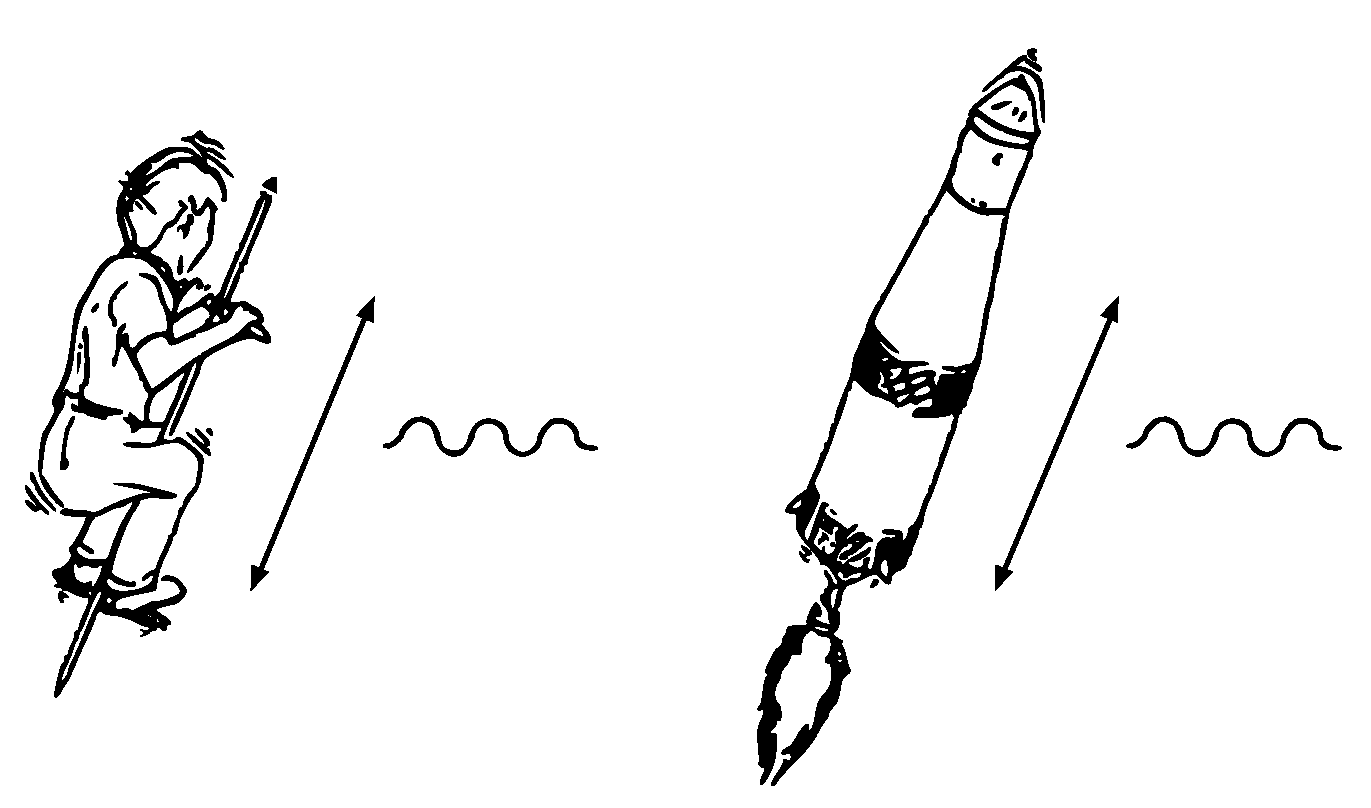
\includegraphics[width=.65\linewidth]{POGO-Analog}
  \caption{POGO比拟示意图}\label{POGO-Analog}
\end{figure}

\begin{figure}[th]
  \centering
  % %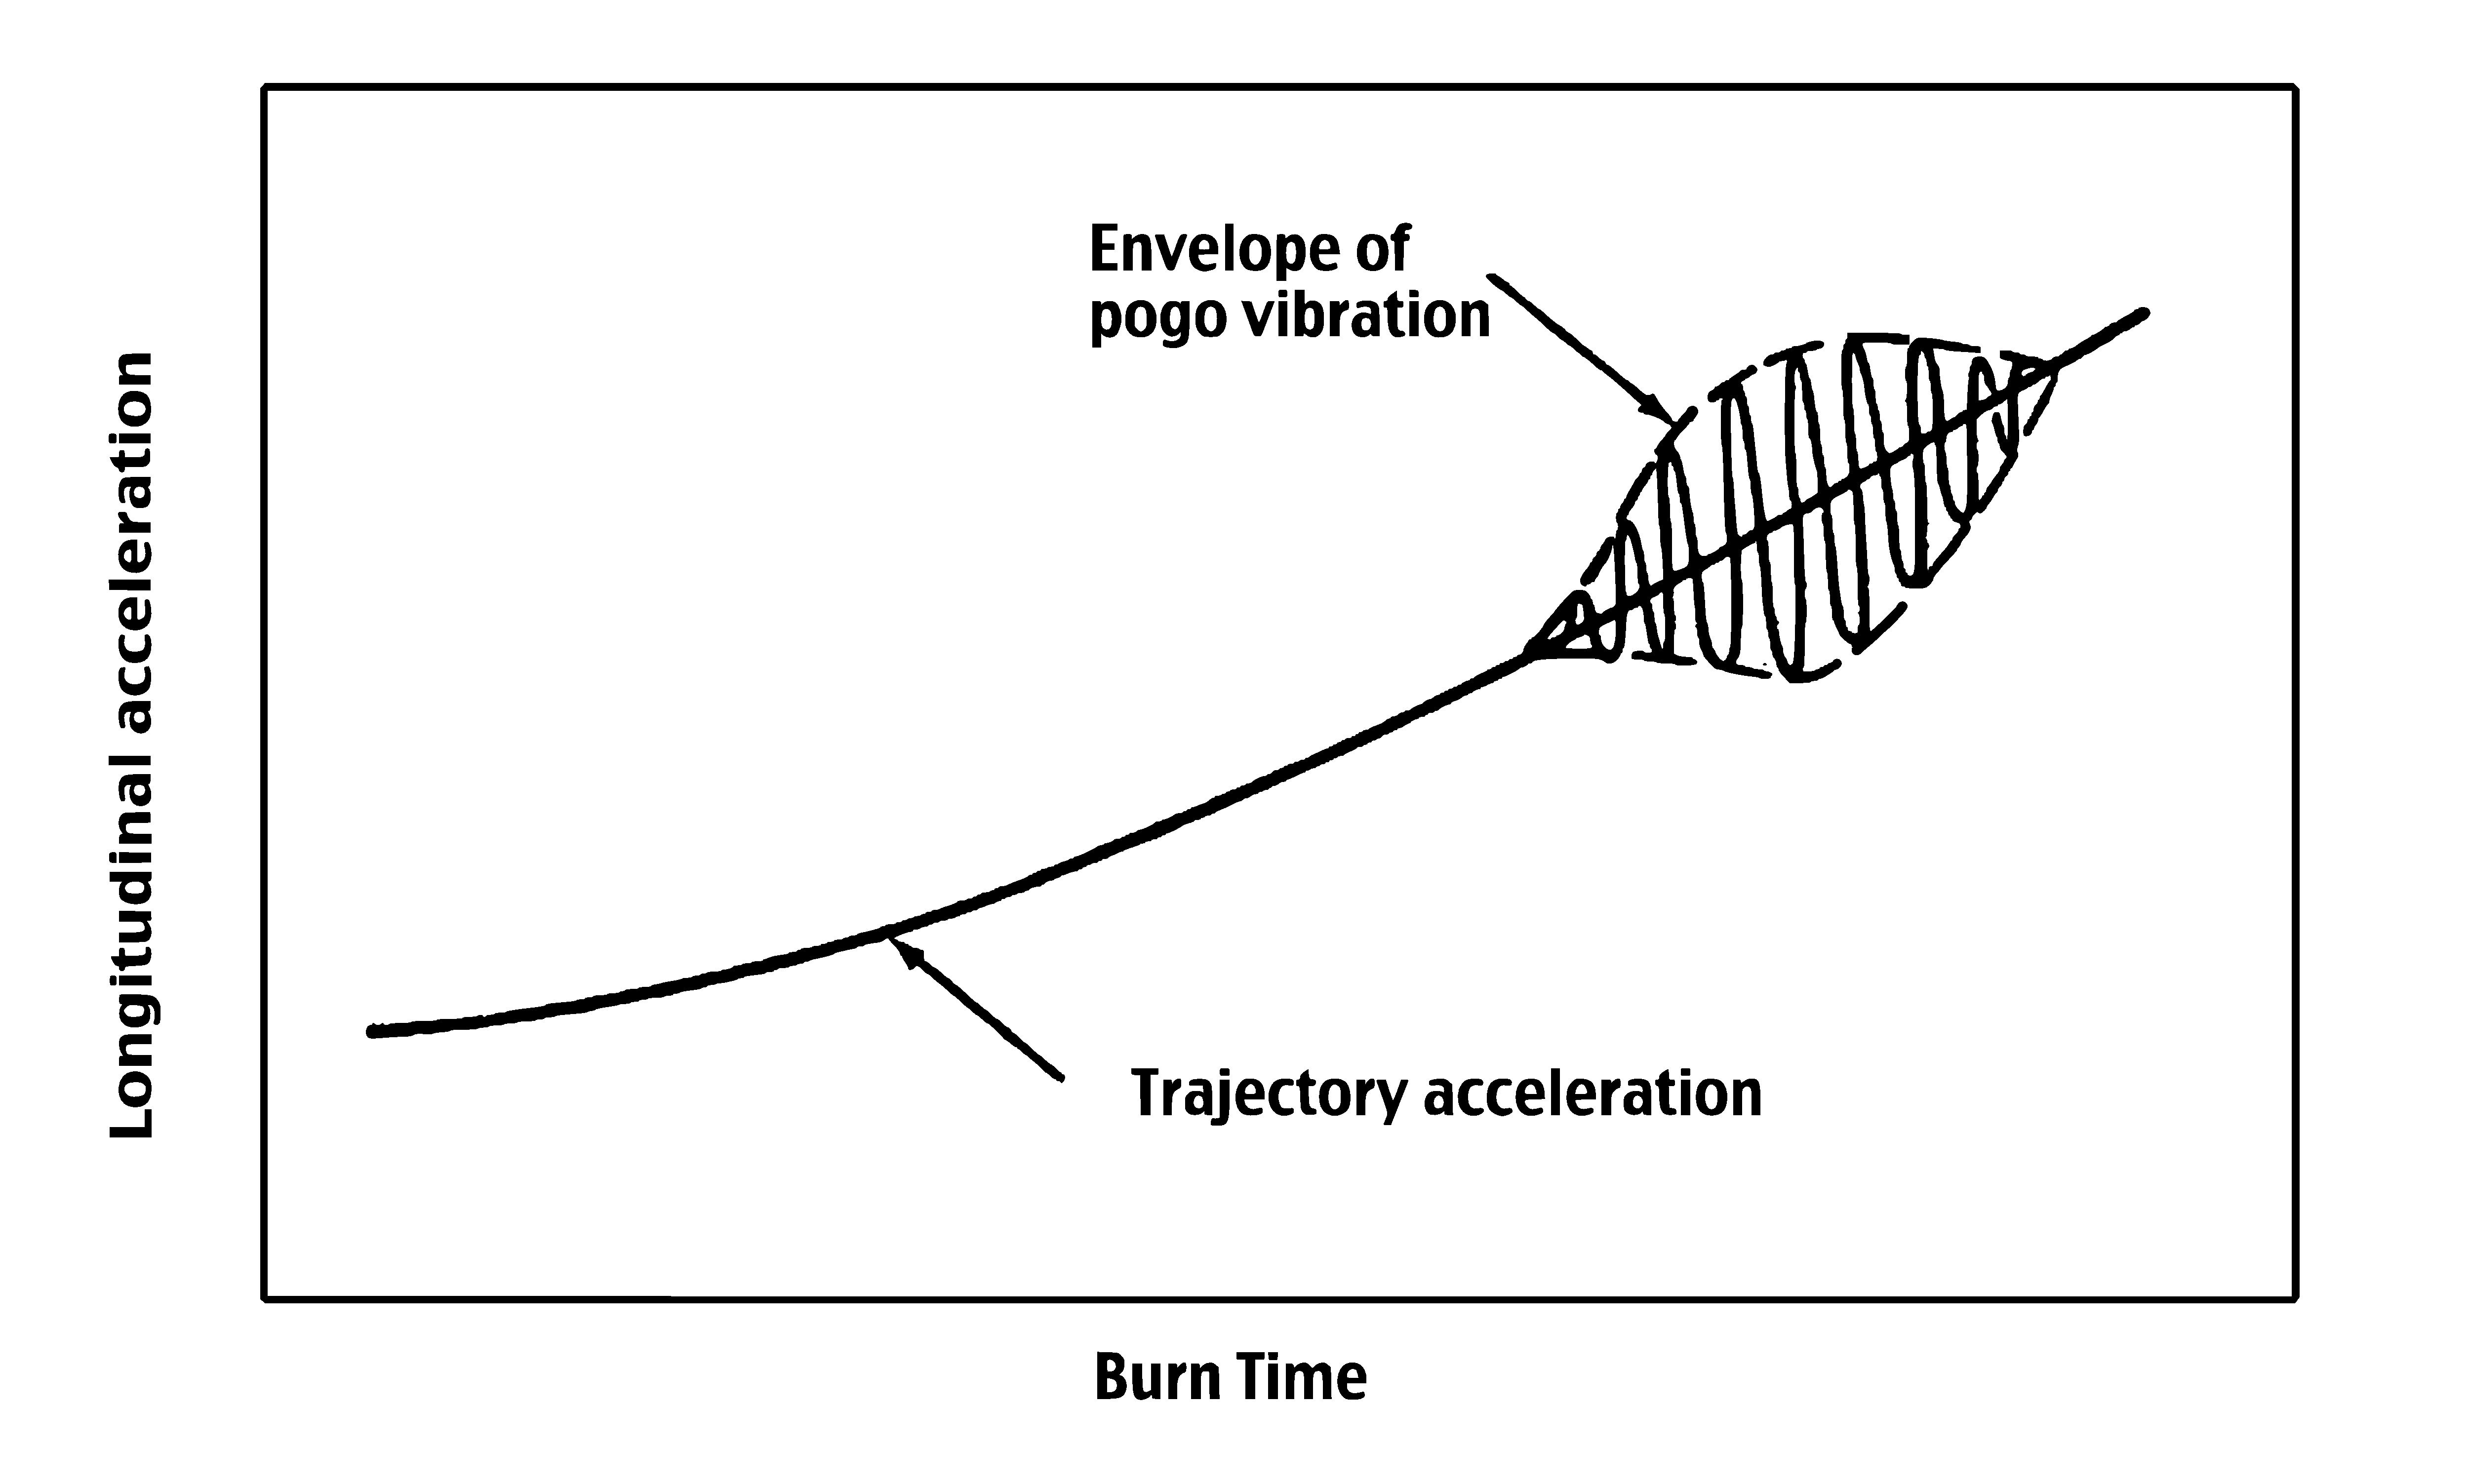
\includegraphics[width=.75\linewidth]{POGO-Typical.pdf}
  \caption{典型纵向耦合振动的时域历程}\label{Typical:POGO}
\end{figure}

纵观现代火箭工程发展史,POGO振动有害于人类航天飞行的典型例证当属美国土星V运载器的一系列发射经历\cite{Hill:1969, Rich:1969, Jarvinen:1970}。土星V运载火箭是美国最大的运载器,是美国国家航空航天局(NASA)在阿波罗计划和天空实验室两项太空计划中使用的多级可抛式液态燃料火箭。事实上,在其总共多达十三次的发射经历中,数次都受到了POGO振动问题的困扰\cite{Larsen:2008}。在1968年土星V编号AS-502次的发射过程中,液体火箭一级推进器(图\ref{SaturnV-Stage1})在工作段105$\sim$140秒内发生了振动频率为5.3Hz,幅值约0.33g的POGO振动。振动导致了五个发动机推力不同步,最终使得飞船登月舱裙部壁板发生开裂。同年十二月发射的土星AS-503,在发动机关机前50秒出现了振动频率为18Hz的POGO振动。事后调查表明,此次主发动机机架与贮箱底部产生的谐振虽然没有传递到火箭壳体,但是已经非常接近简体结构的设计强度极限。在1969年第AS-507次飞行中,液体火箭二级发动机在工作期间出现了四次严格意义上的POGO 振动,所幸最终都被结构系统的非线性效应所遏制。然而,在1970年土星V执行阿波罗13号任务的时候(AS-508),严重的POGO振动导致主发动机机架产生了频率为16Hz,加速度高达68g的失稳现象。由于燃烧室内压力脉动过于剧烈,火箭中部的5号推进器在二级火箭燃烧过程中发生了提前关闭(图\ref{SaturnV-Stage1}),最终导致登月任务被迫放弃,调查发现发动机机架总共被拉长了约7.6厘米。除此之外,宇宙神、大力神和雷神等航空运载器也都在各自发射过程中出现了或多或少的POGO振动\cite{Walker:1964, Wagner:1970, Oppenheim:1993};而法国钻石B火箭更是在其初次发射的五次飞行中都遇到了POGO振动,并且箭体上部分位置的振动量级已然高达足以导致运载器或者卫星结构发生破坏的20$\sim$30g\cite{Dordain:1974}。反观我国的航天事业,在2003年运载火箭长征2F第五次飞行中,遥测数据与宇航员的感受均显示一级助推器飞行末期火箭产生了比较强烈的振动\cite{Ma-Daoyuan:2010, Rong-Kelin:2011}。

\begin{figure}[t]
  \begin{center}
    \begin{minipage}{.47\linewidth}
      %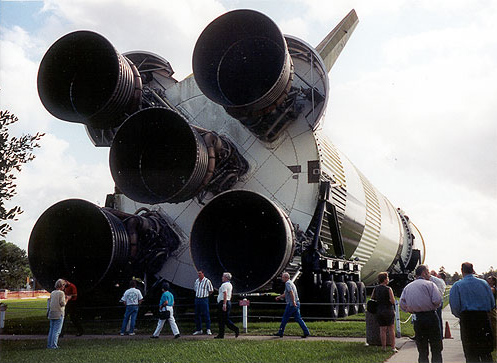
\includegraphics[width=\linewidth]{SaturnV-Stage1.jpg}
      \caption{土星V一级推进器 S-IC}\label{SaturnV-Stage1}
    \end{minipage}
    \begin{minipage}{.47\linewidth}
      %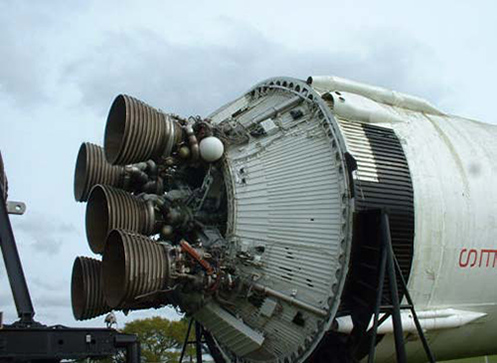
\includegraphics[width=\linewidth]{SaturnV-Stage2.jpg}
      \caption{土星V二级推进器提前关闭}\label{SaturnV-Stage2}
    \end{minipage}
  \end{center}
\end{figure}

POGO振动的危害性主要表现在如下几个方面\cite{Rubin:1970, Wang-Qizheng:1999}:
\begin{enumerate}[leftmargin=\parindent, align=parleft, labelindent=0pt, labelwidth=*]
  \item 可使运载器结构系统产生过大的动载荷,造成火箭有效载荷部分损坏,影响主要任务的完成。如法国的“钻石B”运载火箭。
  \item 管路系统产生的脉动压力和脉动流量可以导致运载火箭性能降低,造成任务失败。由于燃烧室压力的剧烈振荡导致出现虚假的推进剂耗尽指示信号,致使发动机过早关车。如美国的“大力神”二号任务失败,“土星V/阿波罗13”运载火箭第二级性能大大降低。
  \item 增加运载器结构载荷,使有效载荷重量受到限制,而不得不重新设计结构。如美国的“雷神/阿金纳”火箭重新设计了“阿金纳”的结构。
  \item 可以导致仪器、惯性仪表、设备和卫星所不允许的振动环境条件。如“雷神/阿金纳”运载火箭“阿金纳”级上的仪器设备需按较大的正弦振动等级重做安全鉴定。
  \item 可以产生宇航员所不能允许的振动条件,使得宇航员的生理系统失调、身体不适,进而不能正常工作。如“双子星座/大力神”运载火箭的宇航员视力模糊,感到不舒服。
\end{enumerate}

根据NASA等机构对人体的测试表明\cite{Creer:1960, Burton:1988, Davis:2008}:垂直状态下正常人体所能承受的G力极限为5g,经过训练的宇航员可以短时承受正9g的最大加速度;在水平方向上,早期实验表明未经训练的人员在20g的加速度下只能坚持少于十秒的时间,10g可以支持一分钟,6g状态则能够维持十分钟。一般来说,短暂的“红视症”(Blackout,负G力)与“黑视症”(Redout,正G力)只是人体自我保护机制产生的警讯,用以警告人体已经濒临极限。倘若继续维持甚至增加G力,脑部将再因保护机制而停止工作产生昏厥,此时位于空中的飞行器即有极度危险;接着,当G力超过人脑所能负荷极限时,人脑将因长时间过度缺氧或充血的血管破裂而造成永久性伤害,最严重的即是因脑部严重损坏而死亡,或是脆弱的内部组织因持续遭受高G力而产生破裂,造成严重出血并危及生命。

可以看出,能否成功抑制甚至消除POGO振动已经成为当代航天运载器的重要设计指标之一,也是人类能否进行宇航飞行的前提之一。所以,目前基本上所有研究大型液体火箭的国家都对这种振动给予了相当大的重视和研究力度。因此,在我国大力发展宇航事业的重大契机下,针对POGO振动稳定性方面的理论分析也变得更加紧迫和必要。

\section{纵向耦合振动问题的主要机理分析}
\label{sec:POGO_Mechanicsm}
从本质上讲,POGO振动是一种由于火箭结构系统和管路推进系统发生相互作用而引起的不稳定振动。这种振动带有明显的流固耦合低频振动特征,属于不稳定的闭环自激振动\cite{Rubin:1973, Doiron:1977, Huang-Huaide:1987}。

\begin{figure}[h]
  \centering
  %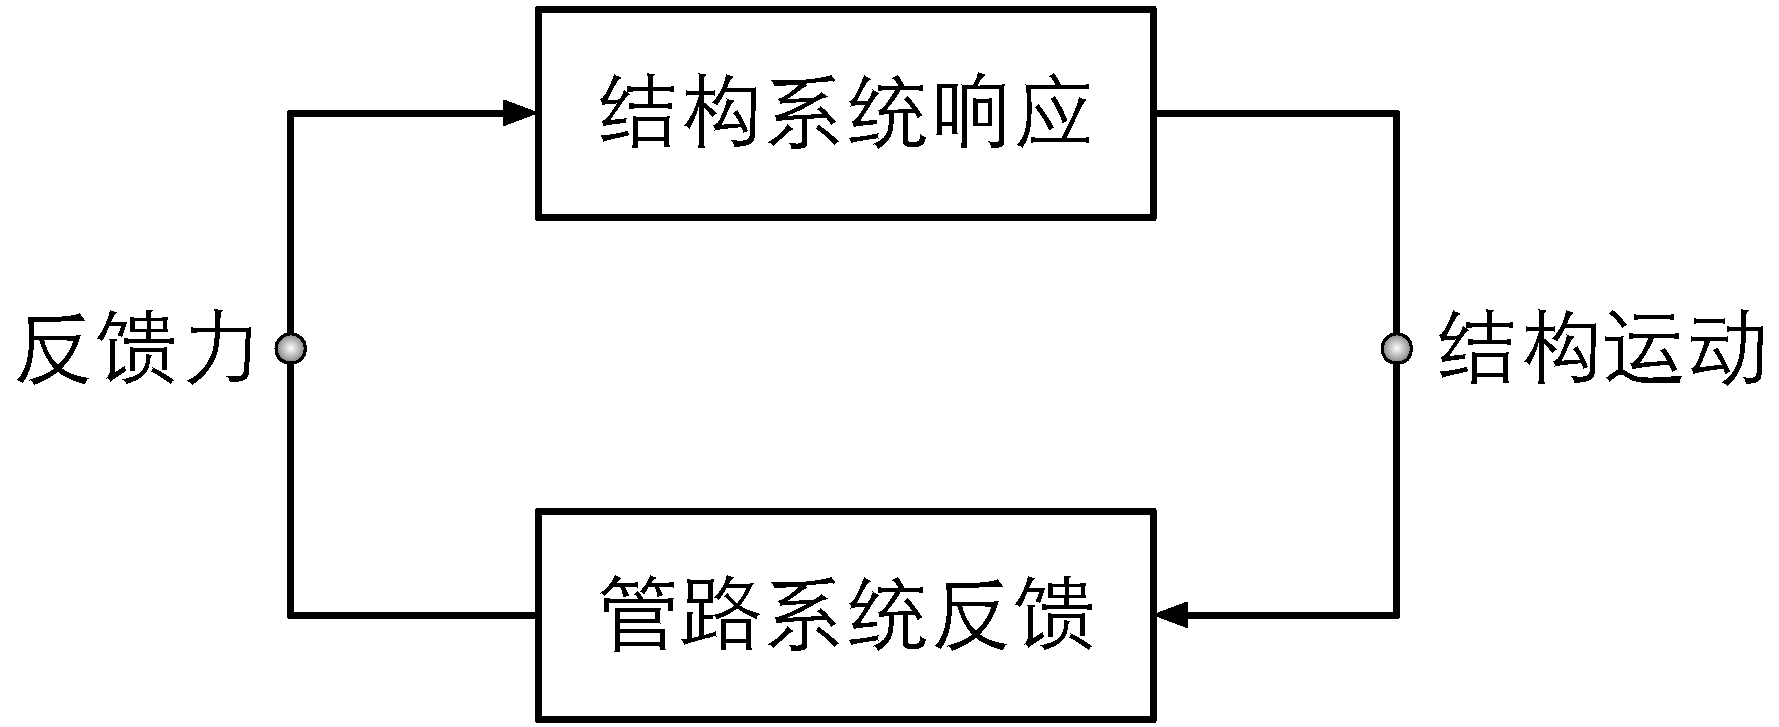
\includegraphics[width=.6\linewidth]{Struture-Feedline-Interaction-Diagram.pdf}
  \caption{POGO振动示意框图}\label{Interaction-Diagram}
\end{figure}

除去一种不常见的增压气体耦合POGO振动\cite{Rubin:1970},典型的POGO闭环振动究其原因可以归纳为如下过程(图\ref{Interaction-Diagram}):在大型液体运载火箭飞行的过程中,燃烧剂和氧化剂输送管路内的液路压力和流量会因为火箭结构系统的扰动而产生脉动。此脉动量经过不同管路元件的层层传递,最终将会到达液体火箭燃烧室,进而引起发动机产生推力脉动。此外,在燃烧剂和氧化剂的输运过程中,管路系统也会由于液体和管壁发生流固耦合作用而产生作用于结构系统上的额外反馈力\cite{About:1987, Paidoussis:1993}。所以当发动机推力脉动,联合上述管路系统反馈力,作为外界扰动力反作用于箭体结构时,火箭结构系统和管路推进系统两者就有可能因为固有频率相接近而产生不断放大耦合作用,从而导致液体推进火箭产生自激的纵向不稳定振动\cite{Rubin:1970, Oppenheim:1993}。

\begin{figure}[!htb]
  \centering
  %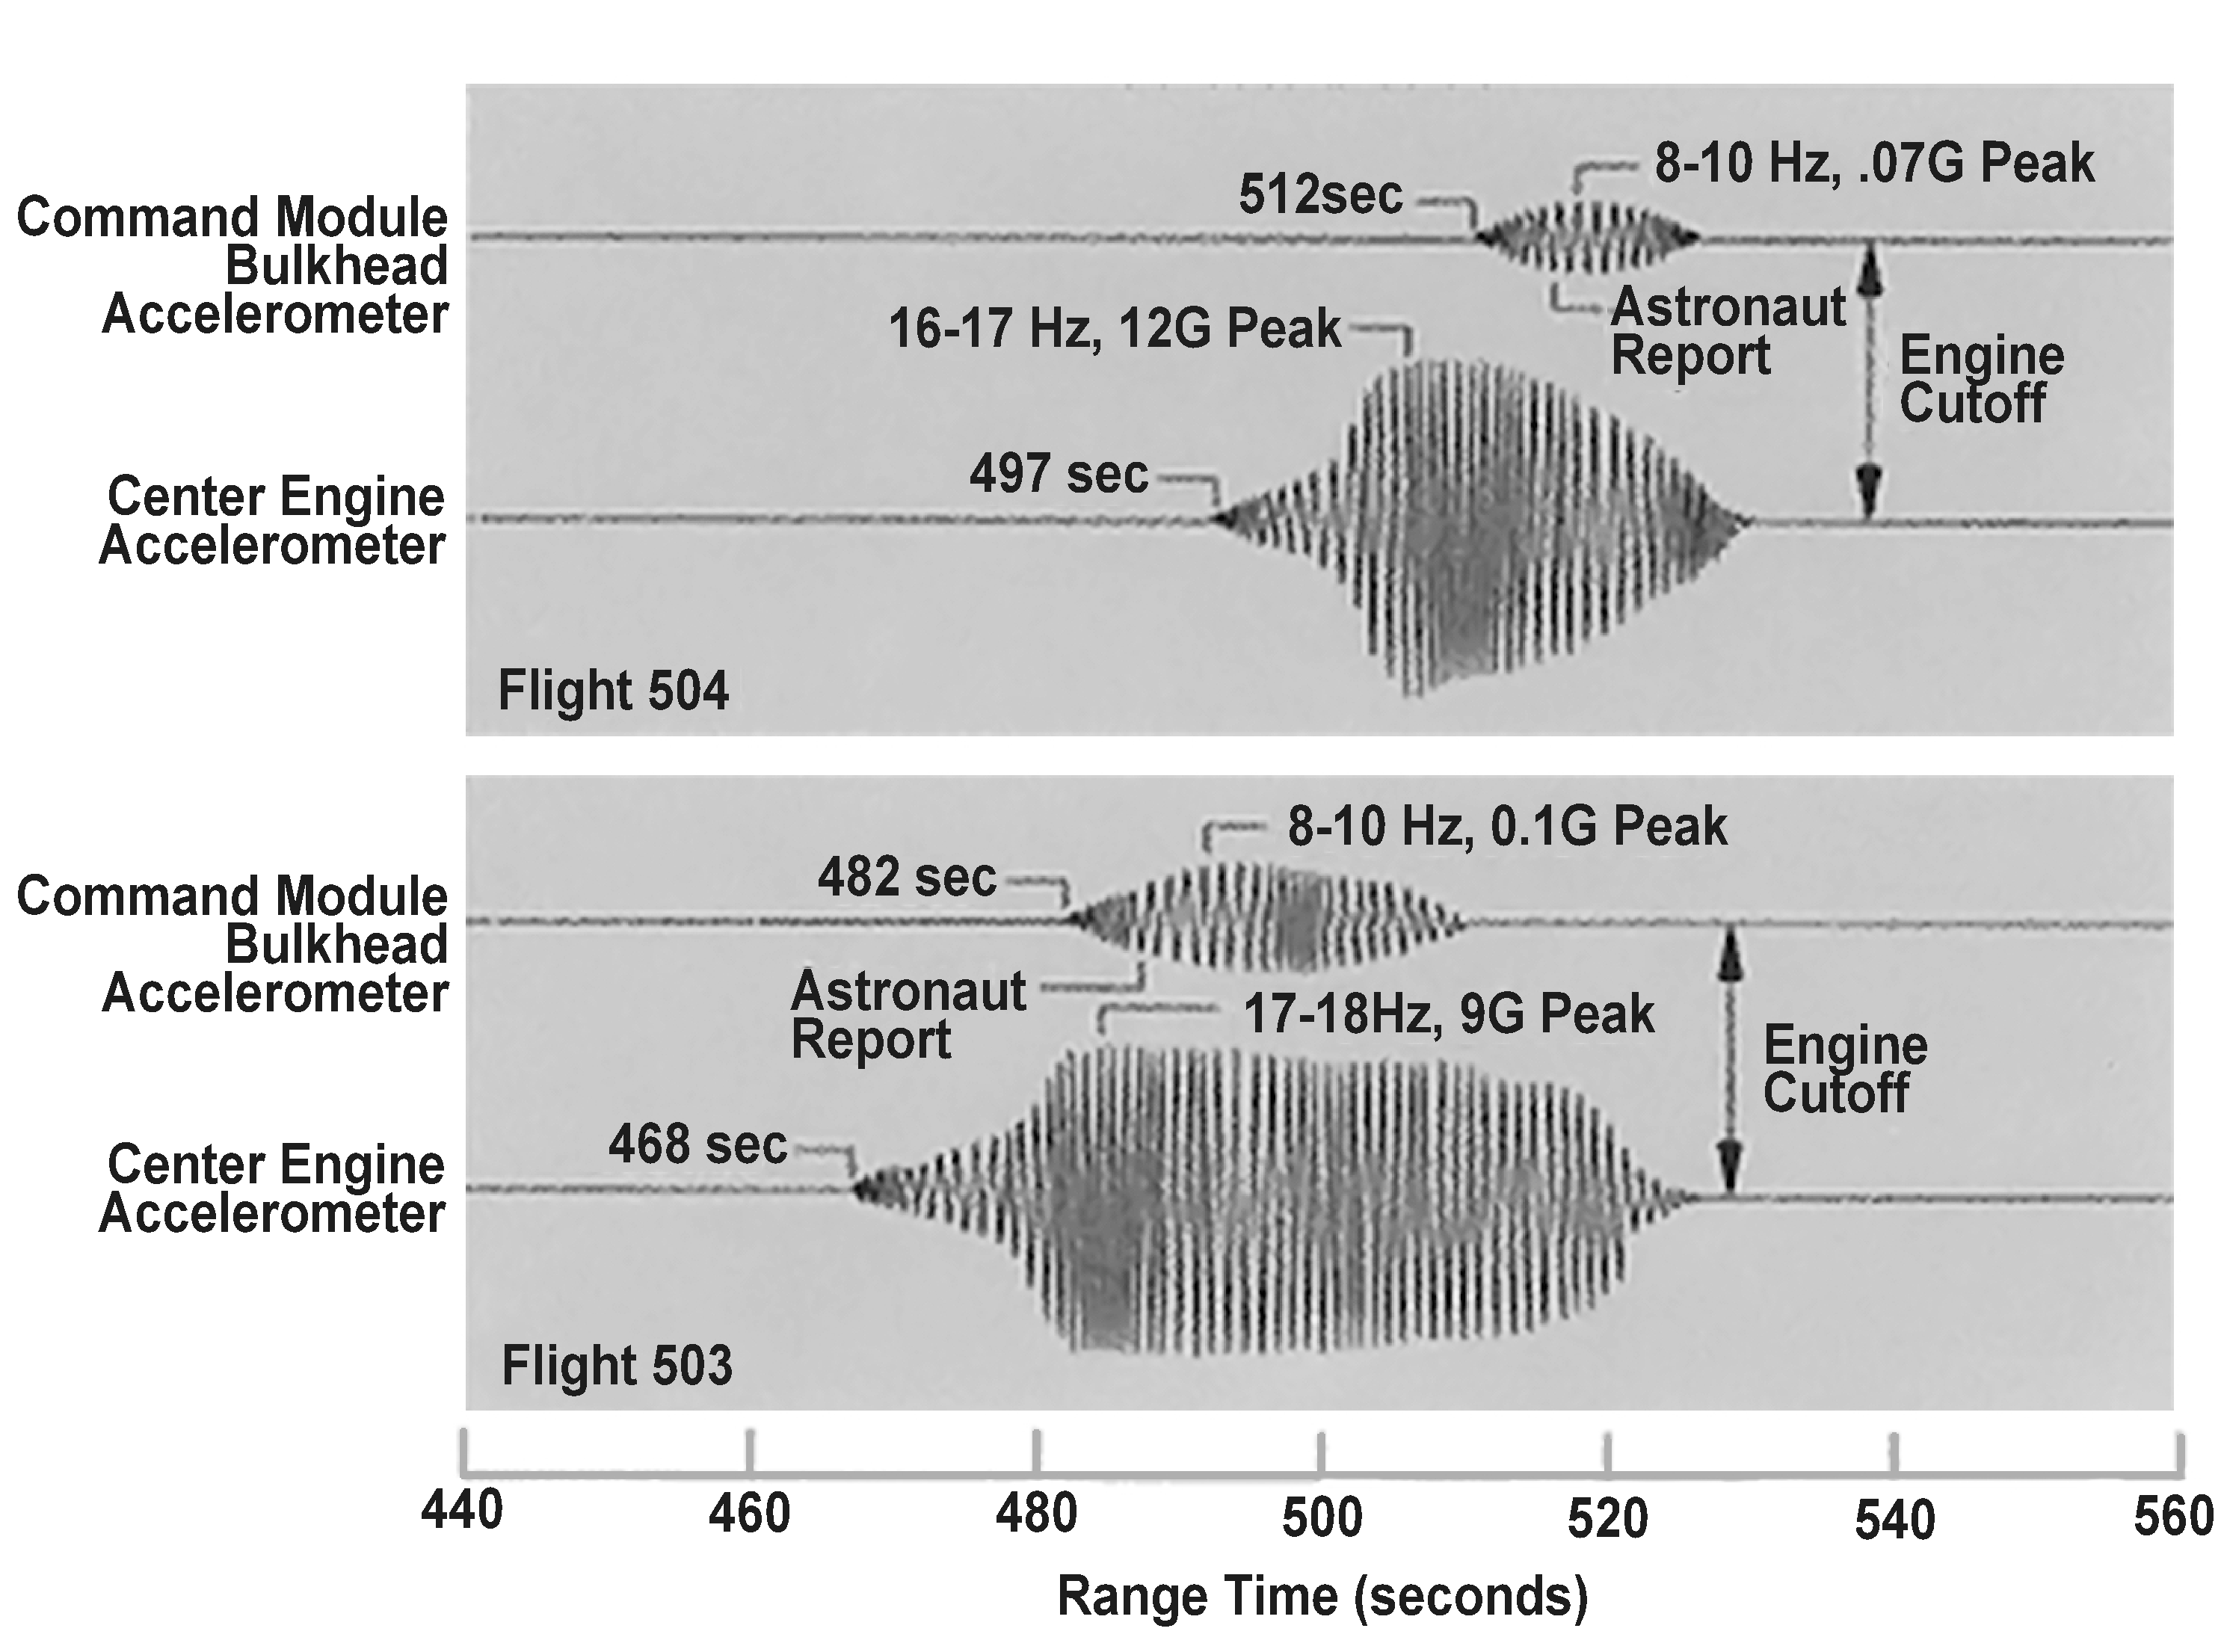
\includegraphics[width=\linewidth]{telemetry-typical.pdf}
  \caption{土星V箭体加速度传感器数据}\label{telemetry-typical}
\end{figure}

参考POGO振动的发生机理并结合国内外大量的飞行遥测数据\cite{Feng-Zhenxing:1981},可以知道这种不稳定振动的发生频率大多与火箭结构系统的低阶纵向振动频率较为接近,其产生和发展过程也表现的十分突然和强烈。事实表明,POGO振动可能发生在液体火箭飞行过程的各个时刻,一次发射也确实可能会出现多次的POGO 振动\cite{Larsen:2008}。然而,由于液体火箭飞行过程是一个持续的变结构参数过程,并且箭体结构在发生较大变形时所引起的非线性效应会打破上面描述的这种频率耦合,所以即使出现POGO 现象,箭体振动的幅值也不会一直发散,而是在其响应时间的历程记录曲线上会出现一个先增大后减小的“鼓包”,典型的遥测POGO振动图像如图\ref{telemetry-typical}所示。鉴于POGO振动从发生到完全消失的时间可能长达数十秒,并且由其引起的箭体纵向振动加速度幅值可能在有效载荷处高达十几甚至几十倍于重力加速度,所以POGO振动对于液体火箭所造成的影响需要根据这种自激振动的量级及持续的时间来进行评价\cite{Wang-Qizheng:1999}。



\section{本文的主要工作}

\begin{figure}[!b]
  \centering
  %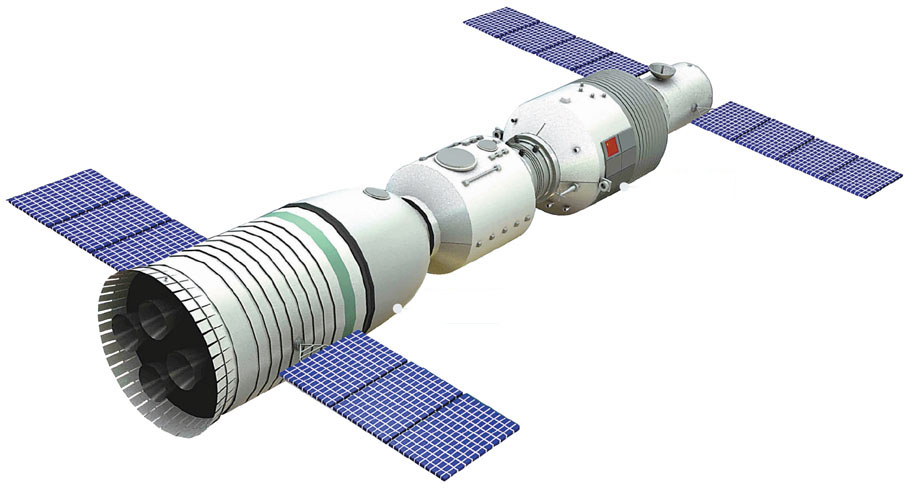
\includegraphics[width=.85\linewidth]{Inter-connect.jpg}
  \caption{神舟十号与天宫一号交汇对接示意图}\label{China-Manned-Flight}
\end{figure}

液体火箭纵向耦合振动问题是一个相对古老却又富含新鲜挑战和契机的复杂系统问题。在我国大力发展航空事业的今天(图\ref{China-Manned-Flight}),更被赋予了深层次的时代意义。传统的液体火箭POGO稳定性分析方法主要分为了矩阵法、单传法和临界阻尼法\cite{Wang-Qizheng:1999}等几类。这些方法都需要先计算出耦合系统的闭环或者开环传递函数,然后通过对系统传递函数进行特征值求解或者绘制Bode和Nyquist图等手段来进行POGO稳定性分析。不过,由于耦合系统的传递函数通常都包含了一些复杂的非线性函数,所以POGO稳定分析的理论难点其实可以被归结为如何快速精确地计算出复杂传递函数的特征值这一经典问题。以矩阵法为例,由于系统反馈力传递矩阵中的元素包含了超越函数和高阶多项式,所以需要对不对称的复数传递矩阵进行非线性复特征值求解,而通常这种非线性方程的求解过程都十分困难并且容易漏根\cite{Dennis:1983, Golub:1996}。正是考虑到此类特征值问题的复杂性,Oppenheim\cite{Oppenheim:1993}等人如前所述,尝试了利用有限元法对管路系统进行直接建模。事实证明,这种方法在处理简单液路元件的组装计算方面确实具有着很高的可操作性和精确度。然而,由于管道内的流体运动问题归根结底是一个复杂的非线性问题\cite{Munson:1990, Paidoussis:1993, Morand:1995},所以当简单流体模型不能够精确描述管路系统传递关系,而研究者们必须要考虑诸如边界层效应,甚至湍流等复杂流体运动的时候,经典的有限元方法就必须被进一步拓展才能适应研究需要,而这种扩展可能相比于直接求解非线性特征值问题更加棘手。除此之外,由于流体单元本构关系的构建严重依赖于液路元件实验参数(如液路惯性,阻抗等)的精确标定,而相比于直接测定各类液路元件的工作参数,标定管路系统的总体反馈力传递函数可能会显得更加方便并且直接。所以,本文在POGO稳定性求解方法的研究方面,直接针对于管路系统的反馈力传递函数展开分析,开辟了另外一种与液路元件有限元组装法平行的POGO振动问题快速特征值求解方法。

为了解决上述主要问题,本文将研究工作分为了以下三个部分:

\begin{enumerate}[label=\textbf{\Roman*.}, align=left, leftmargin=0pt, listparindent=\parindent, itemindent=!, labelwidth=\parindent, labelsep=0pt, itemsep=1em]
  \litem{集中参数模型的POGO稳定性分析(第二章)} 本章主要介绍了液体火箭结构系统和管路推进系统典型液路元件的集中参数模型建模方法,发展了一种基于矩阵法和有理分式拟合法的耦合系统快速特征值求解算法。首先推导了各类管路元件上下游脉动压力、流量之间的传递函数关系,结合发动机燃烧室的压力平衡条件与贮箱底部实际边界条件,综合分析出了管路系统反馈于结构系统的力传递函数。接下来,利用快速特征值求解方法,将包含超越函数的管路推进系统反馈力传递函数等效变换为与结构动力学方程一致的形式,通过求解矩阵特征值问题确定了耦合系统的动力学稳定性问题。最后,通过与传统矩阵法进行计算结果和效率方面的比对,验证了该方法的可靠性和高效性。
  \litem{基于三维带液贮箱模型的POGO稳定性分析(第三章)} 为了更好的模拟火箭贮箱内液体和结构系统之间的流固耦合效应,引入液体火箭贮箱的三维轴对称模型建模方法,并利用虚质量法对贮箱内的液体进行动力学比拟。发展后的三维带液贮箱模型为管路系统提供了更为科学和精确的入口端边界条件,可以同样利用第二章中描述的管路系统类结构化建模方法,结合MSC.Nastran提供的传递函数TF卡建模工具,将拟合完毕的管路系统传递函数与不同类型的结构系统模型进行耦合计算。通过直接计算耦合系统的复特征值问题,可以方便的得知耦合系统的POGO稳定性。此外,计算过程还考虑了POGO稳定性分析中的另外一项关键性技术,即结构系统阻尼特性的识别和建模。带液贮箱的模态实验表明:在满箱、半箱和空箱等不同状态下,火箭结构系统的阻尼特性存在着较大差异,且半箱状态下结构阻尼较其他状态有明显增大。通过调整贮箱干/湿面材料随时间变化的比例阻尼系数,计算模型成功模拟了上述模态实验结果。最终,通过与实际火箭发射的遥测数据进行对比,证明了本套方法可以快速准确的得出POGO出现时间和振动特性。
  \litem{液体火箭POGO稳定性参数分析及传递特性分析(第四章)} 通过比较不同工况下液体火箭POGO稳定性分析结果,本章首先揭示了耦合系统特征值与管路系统关键参数(如蓄压器容积等)之间的相互联系。分析表明,作为POGO抑制器的蓄压器,其容积变化能够显著影响液体火箭管路系统的固有频率,继而改变耦合系统的POGO稳定性。此外,通过比较不同类型液体火箭的历史遥测数据,可以发现有效载荷(如卫星等)的实际振动状态与液体火箭整体POGO振动的强弱并不存在简单的线性关系,单纯的耦合系统特征值计算并不能完全展现液体火箭各处的真实振动状态。文章最后指出,若要使得POGO稳定性分析能够给予未来的发射任务以实质性指导意见,还需综合考虑耦合系统的加速度传递特性分析。
\end{enumerate}
% 
% !TEX encoding = UTF-8 Unicode
%!TEX TS-program = xelatex

\chapter{分子动力学计算热导率}

\section{分子动力学}
\label{sec:Lumped-Feedline-Model}
\begin{figure}[!htb]
  \centering
  \begin{minipage}[b]{0.3\textwidth}
    \centering
    %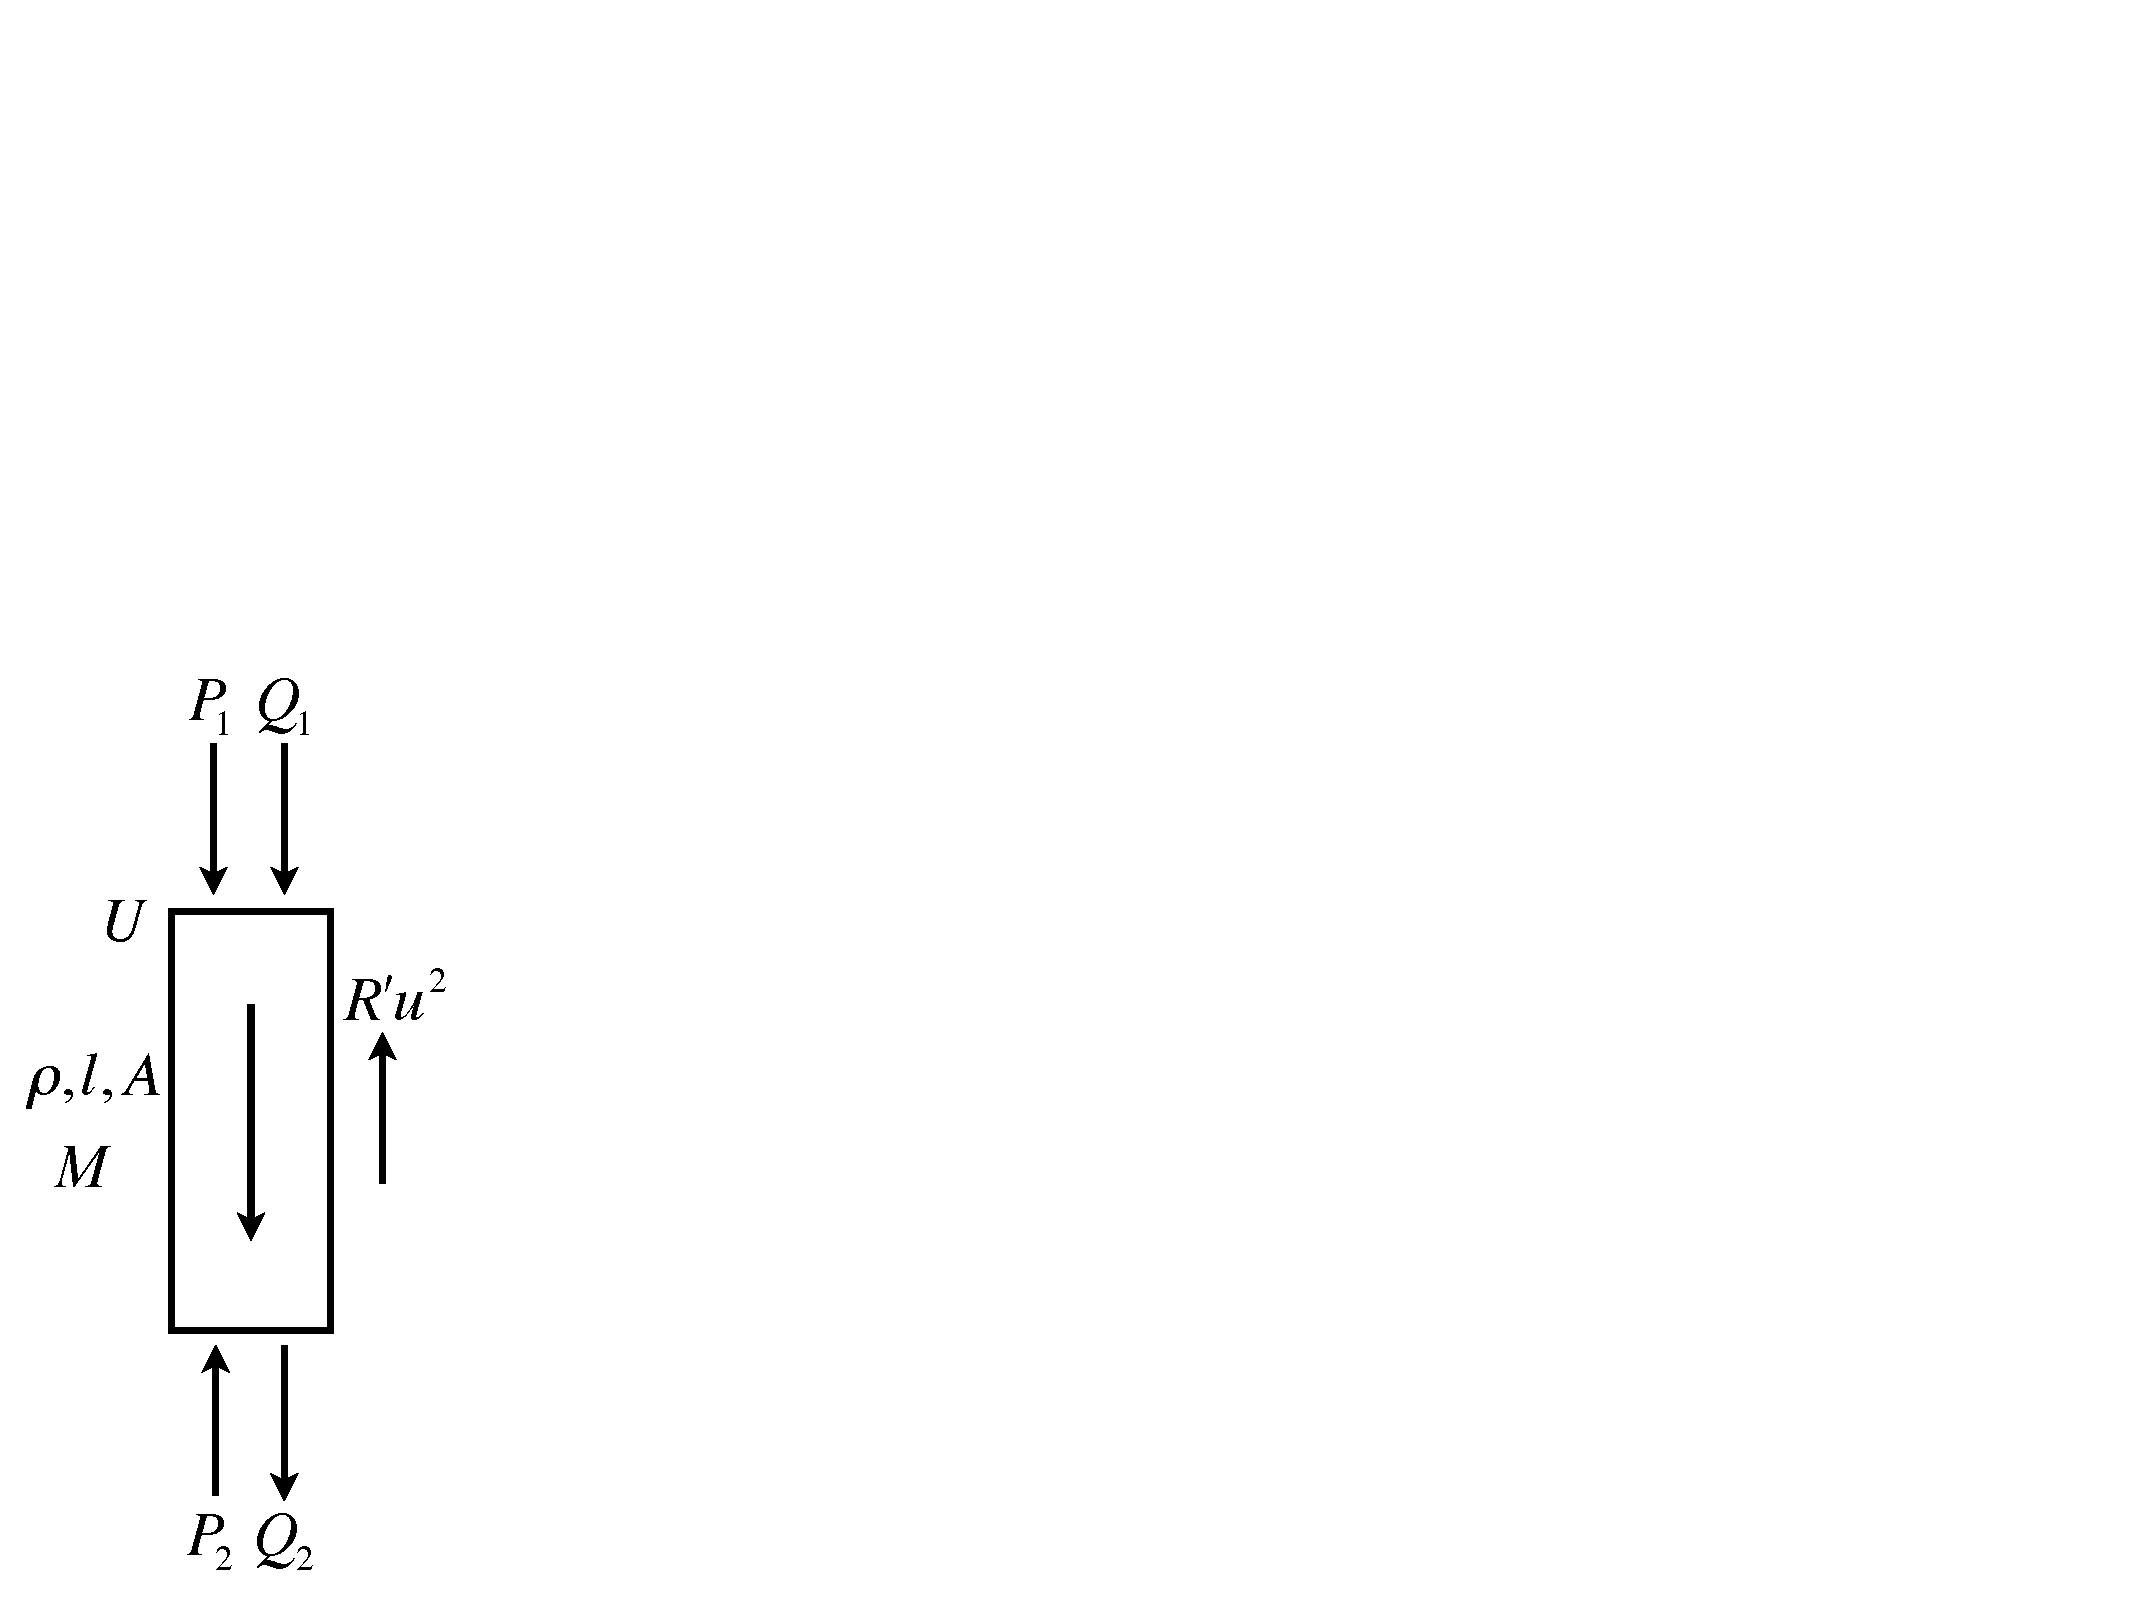
\includegraphics[width=1.2in]{Straight-Tube.pdf}
    \caption*{(a) 输液直管}
  \end{minipage}
  \centering
  \begin{minipage}[b]{0.3\textwidth}
    \centering
    %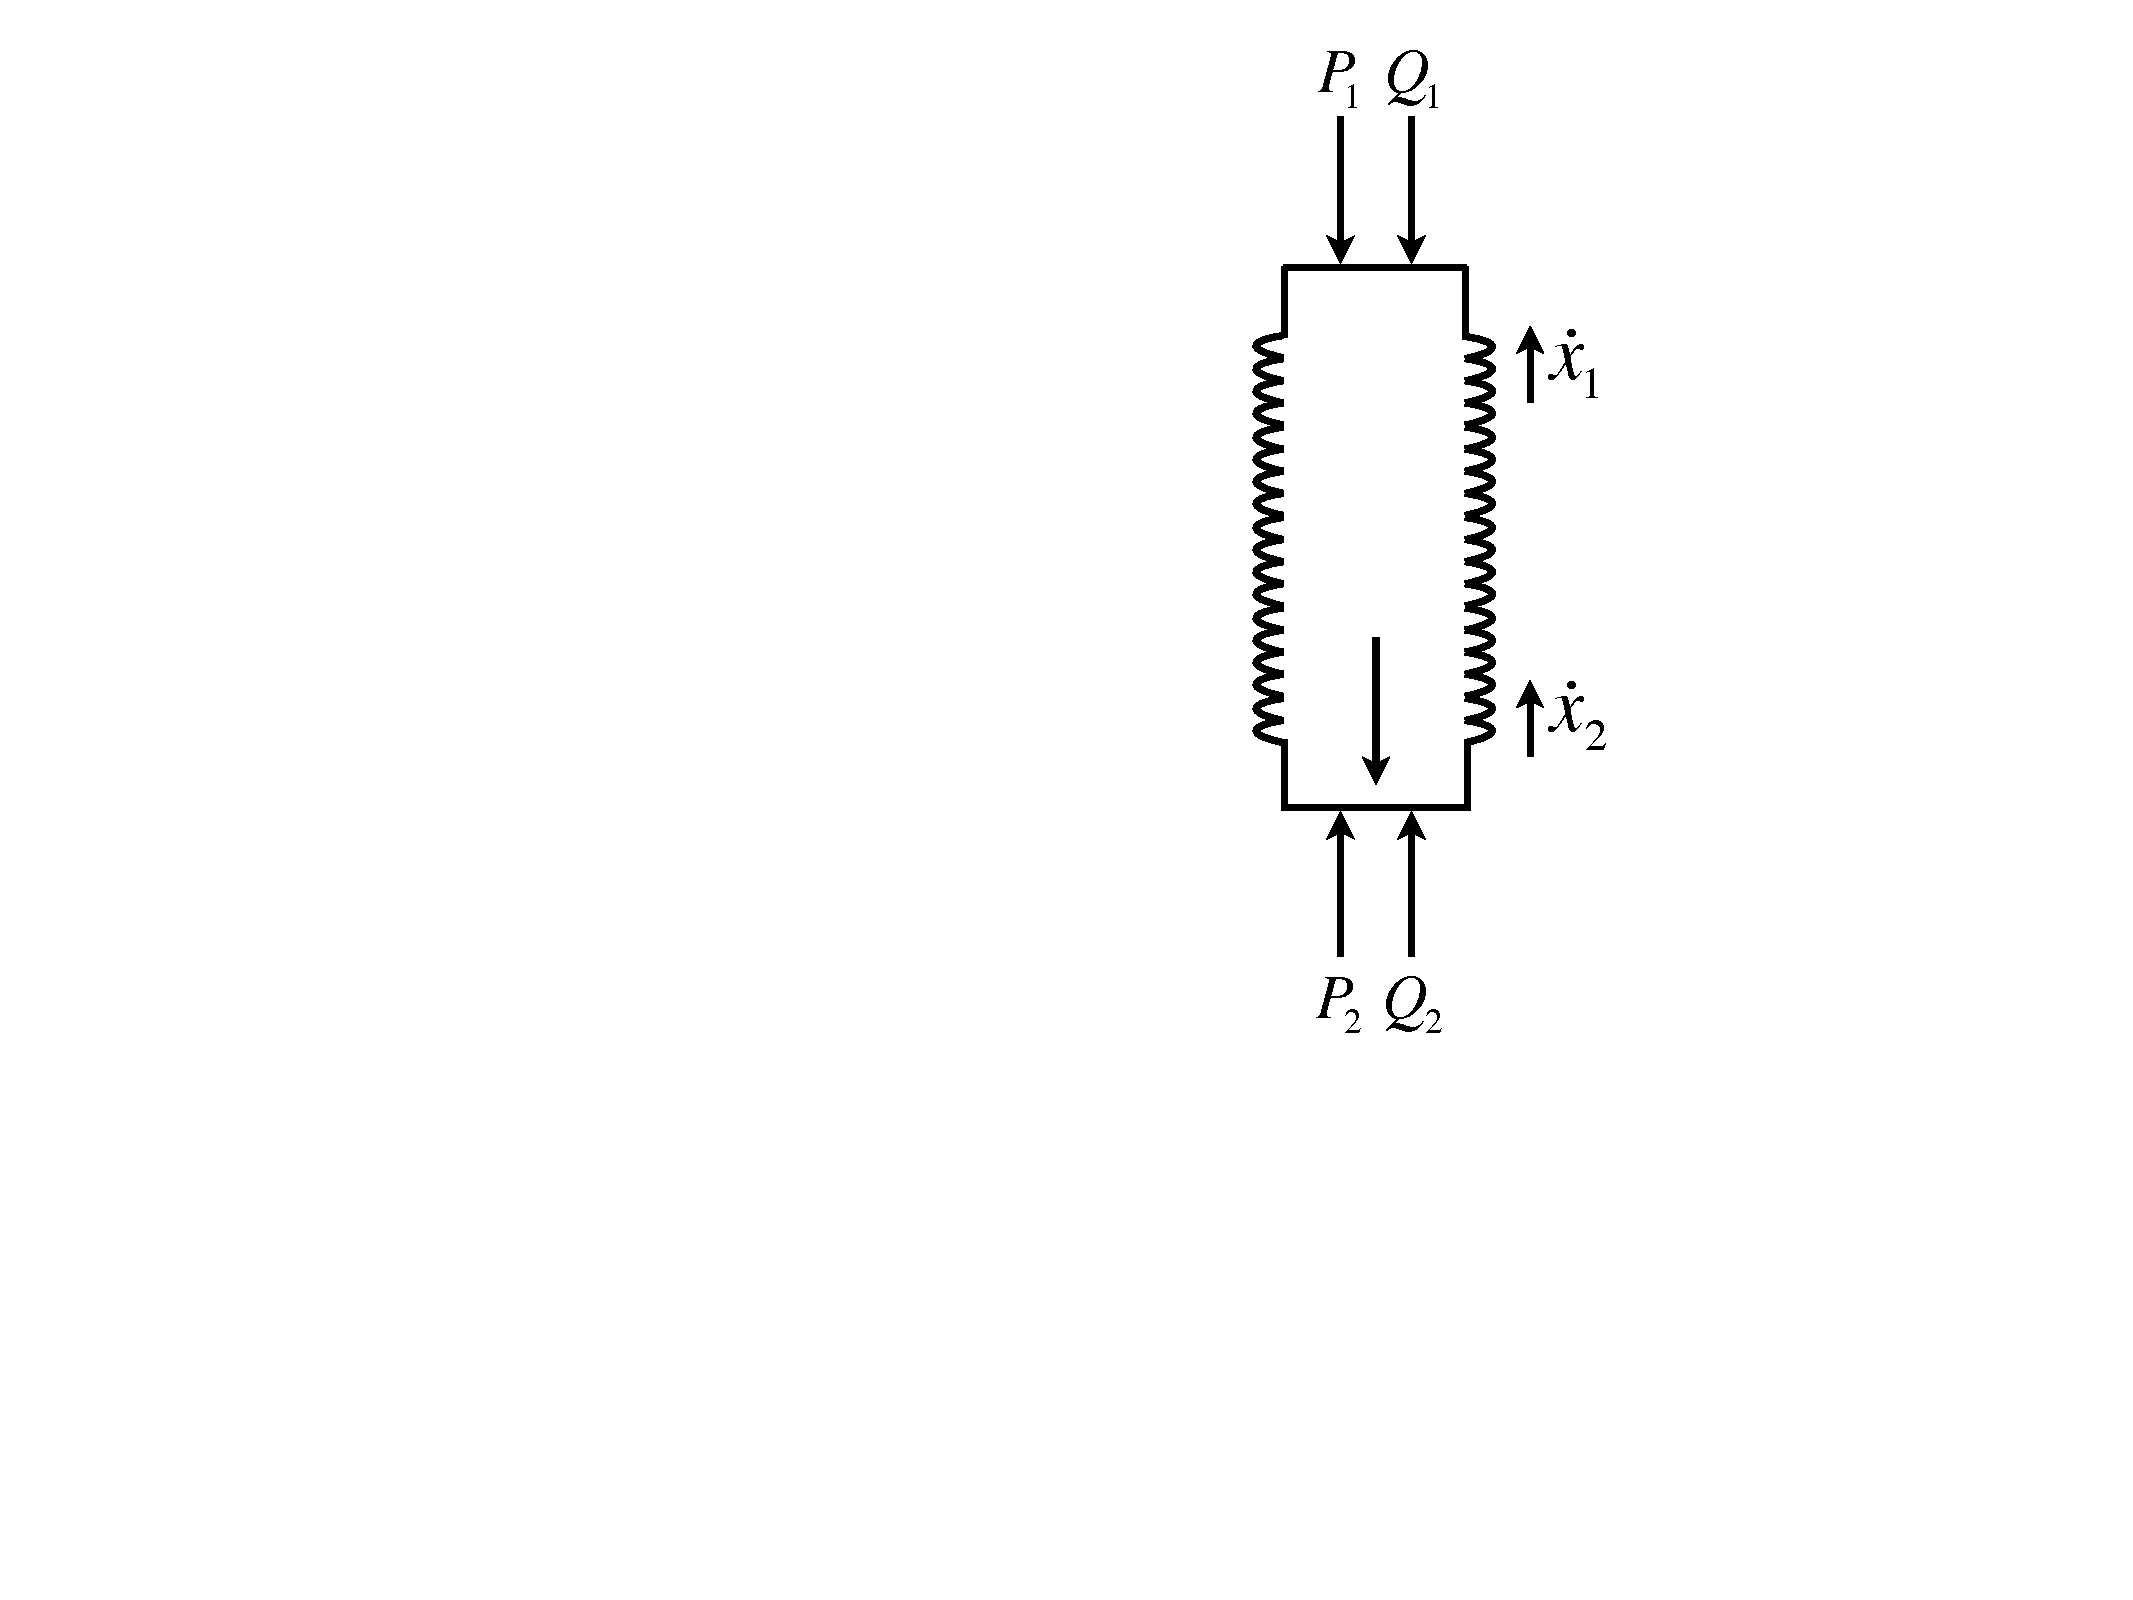
\includegraphics[width=1in]{Bellow.pdf}
    \caption*{(b) 波纹管}
  \end{minipage}
  \centering
  \begin{minipage}[b]{0.3\textwidth}
    \centering
    %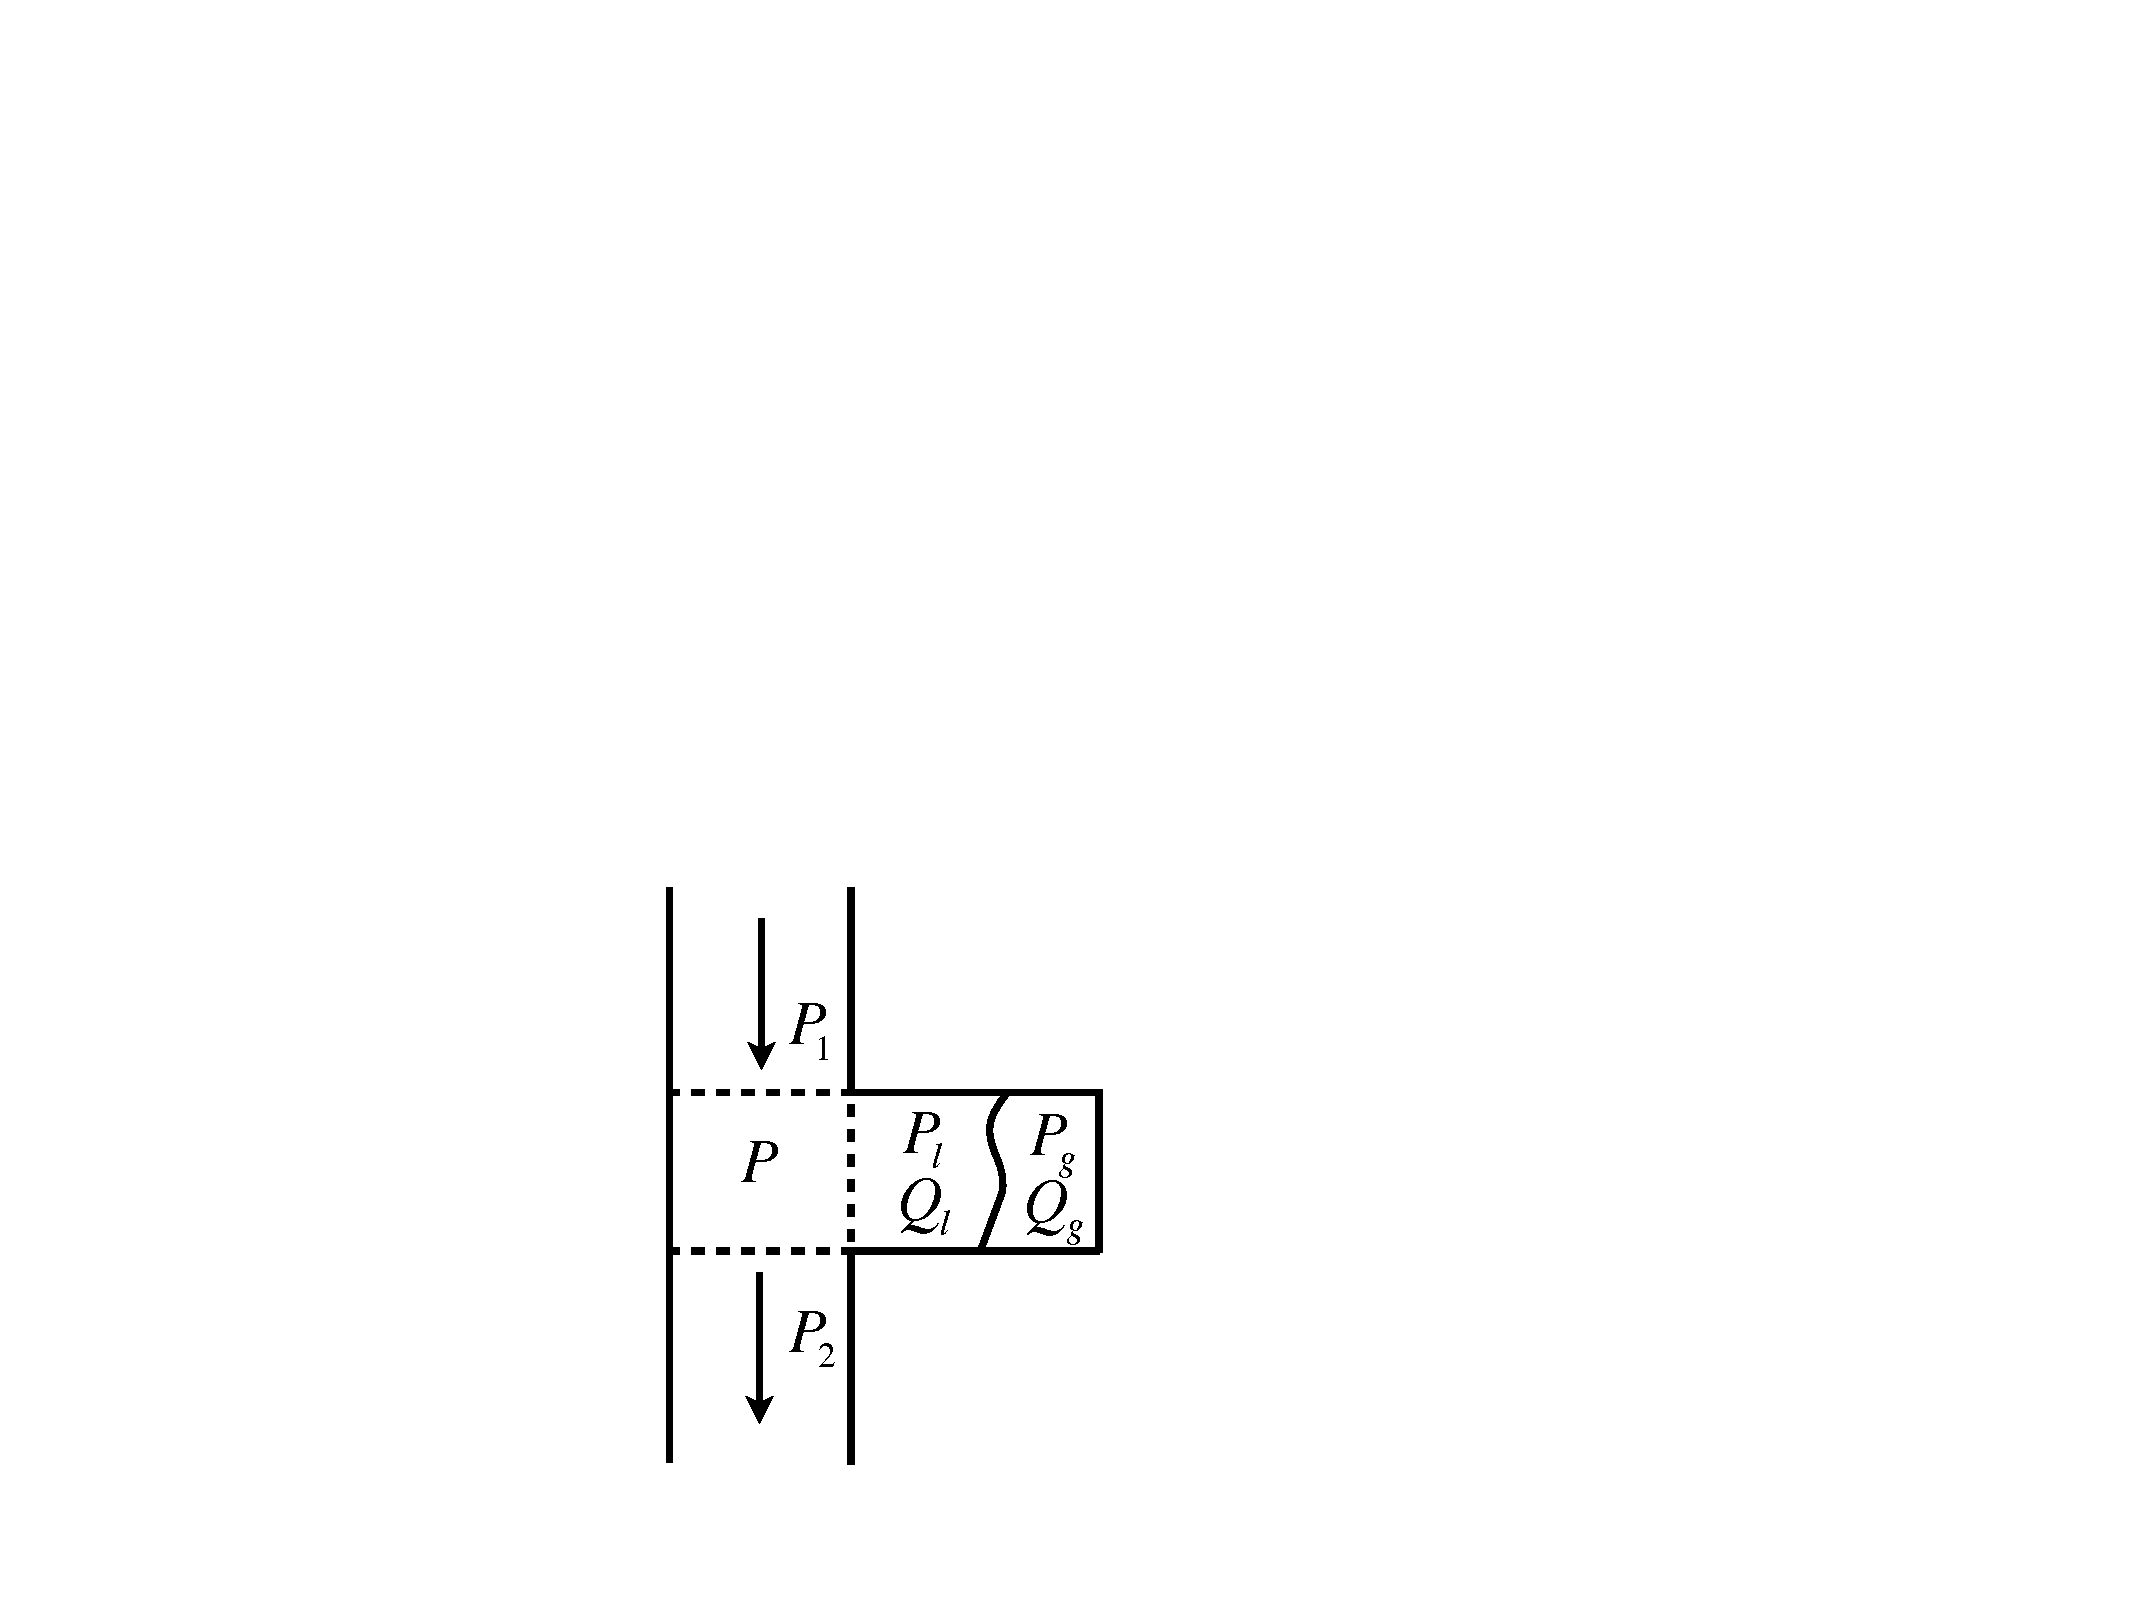
\includegraphics[width=1.5in]{Accumulator.pdf}
    \caption*{(c) 蓄压器}
  \end{minipage}
  \centering
  \begin{minipage}[b]{0.3\textwidth}
    \centering
    %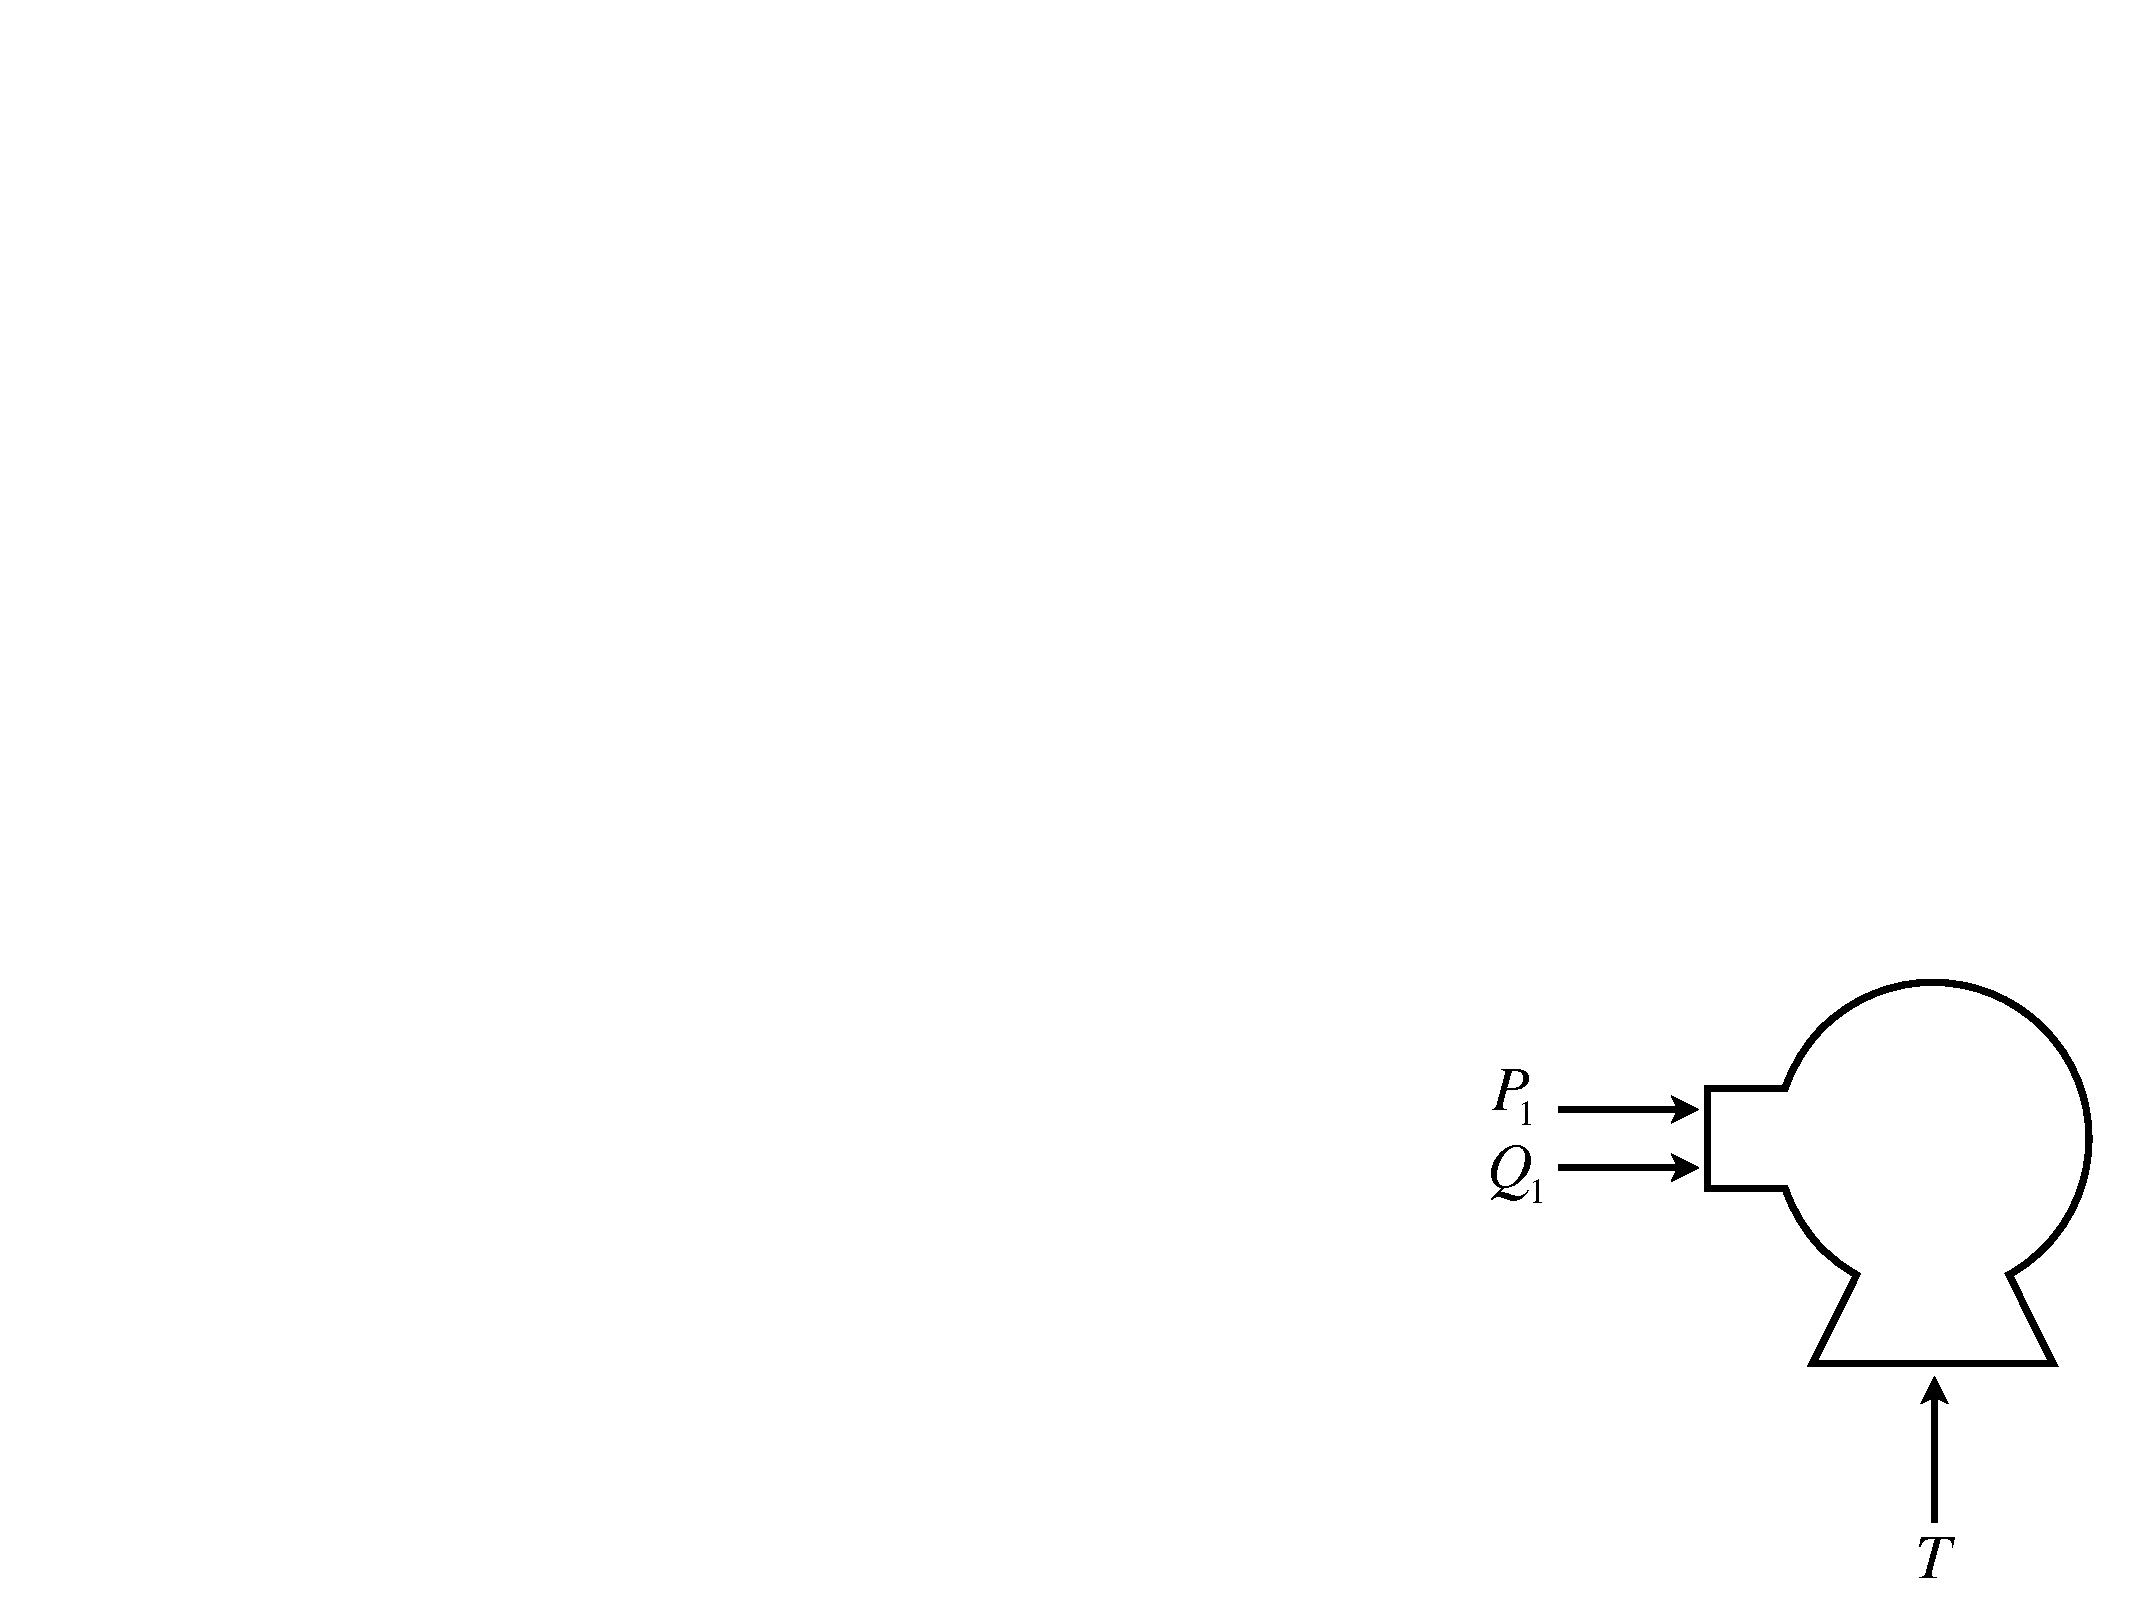
\includegraphics[width=1.6in]{Thrust.pdf}
    \caption*{(d) 推力室}
  \end{minipage}
  \centering
  \begin{minipage}[b]{0.3\textwidth}
    \centering
    % %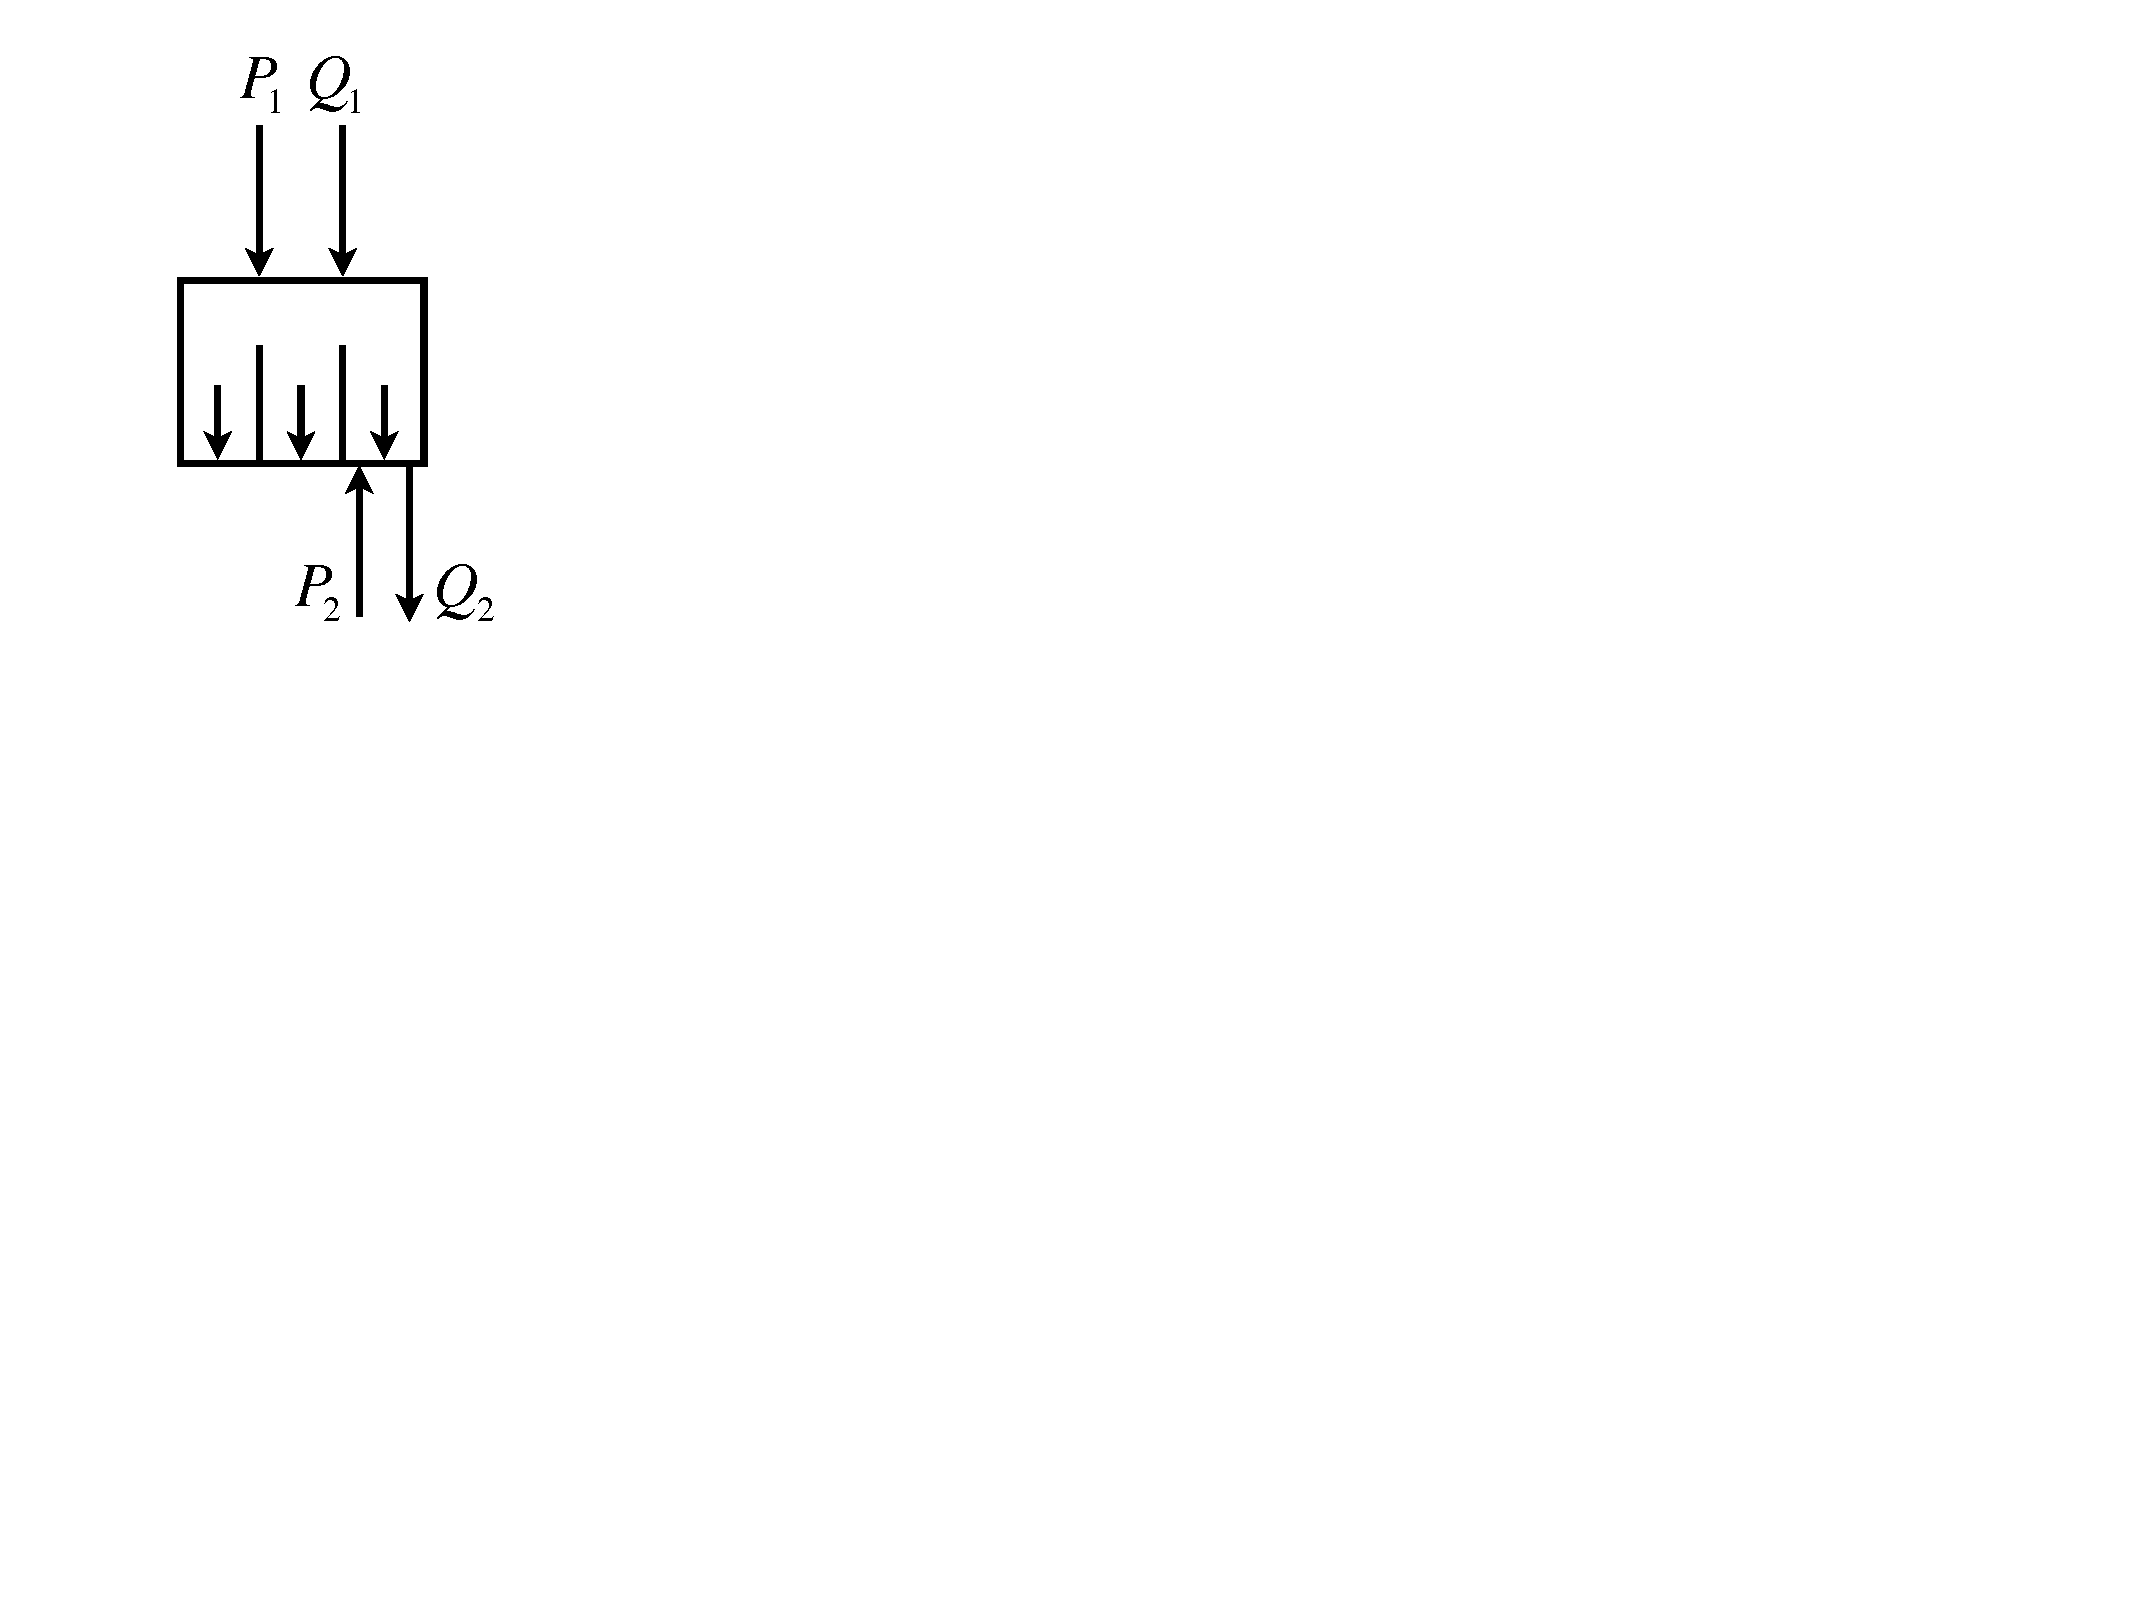
\includegraphics[width=1in]{Multiplex.pdf}
    \caption*{(e) 多通连接器}
  \end{minipage}
  \centering
  \begin{minipage}[b]{0.3\textwidth}
    \centering
    %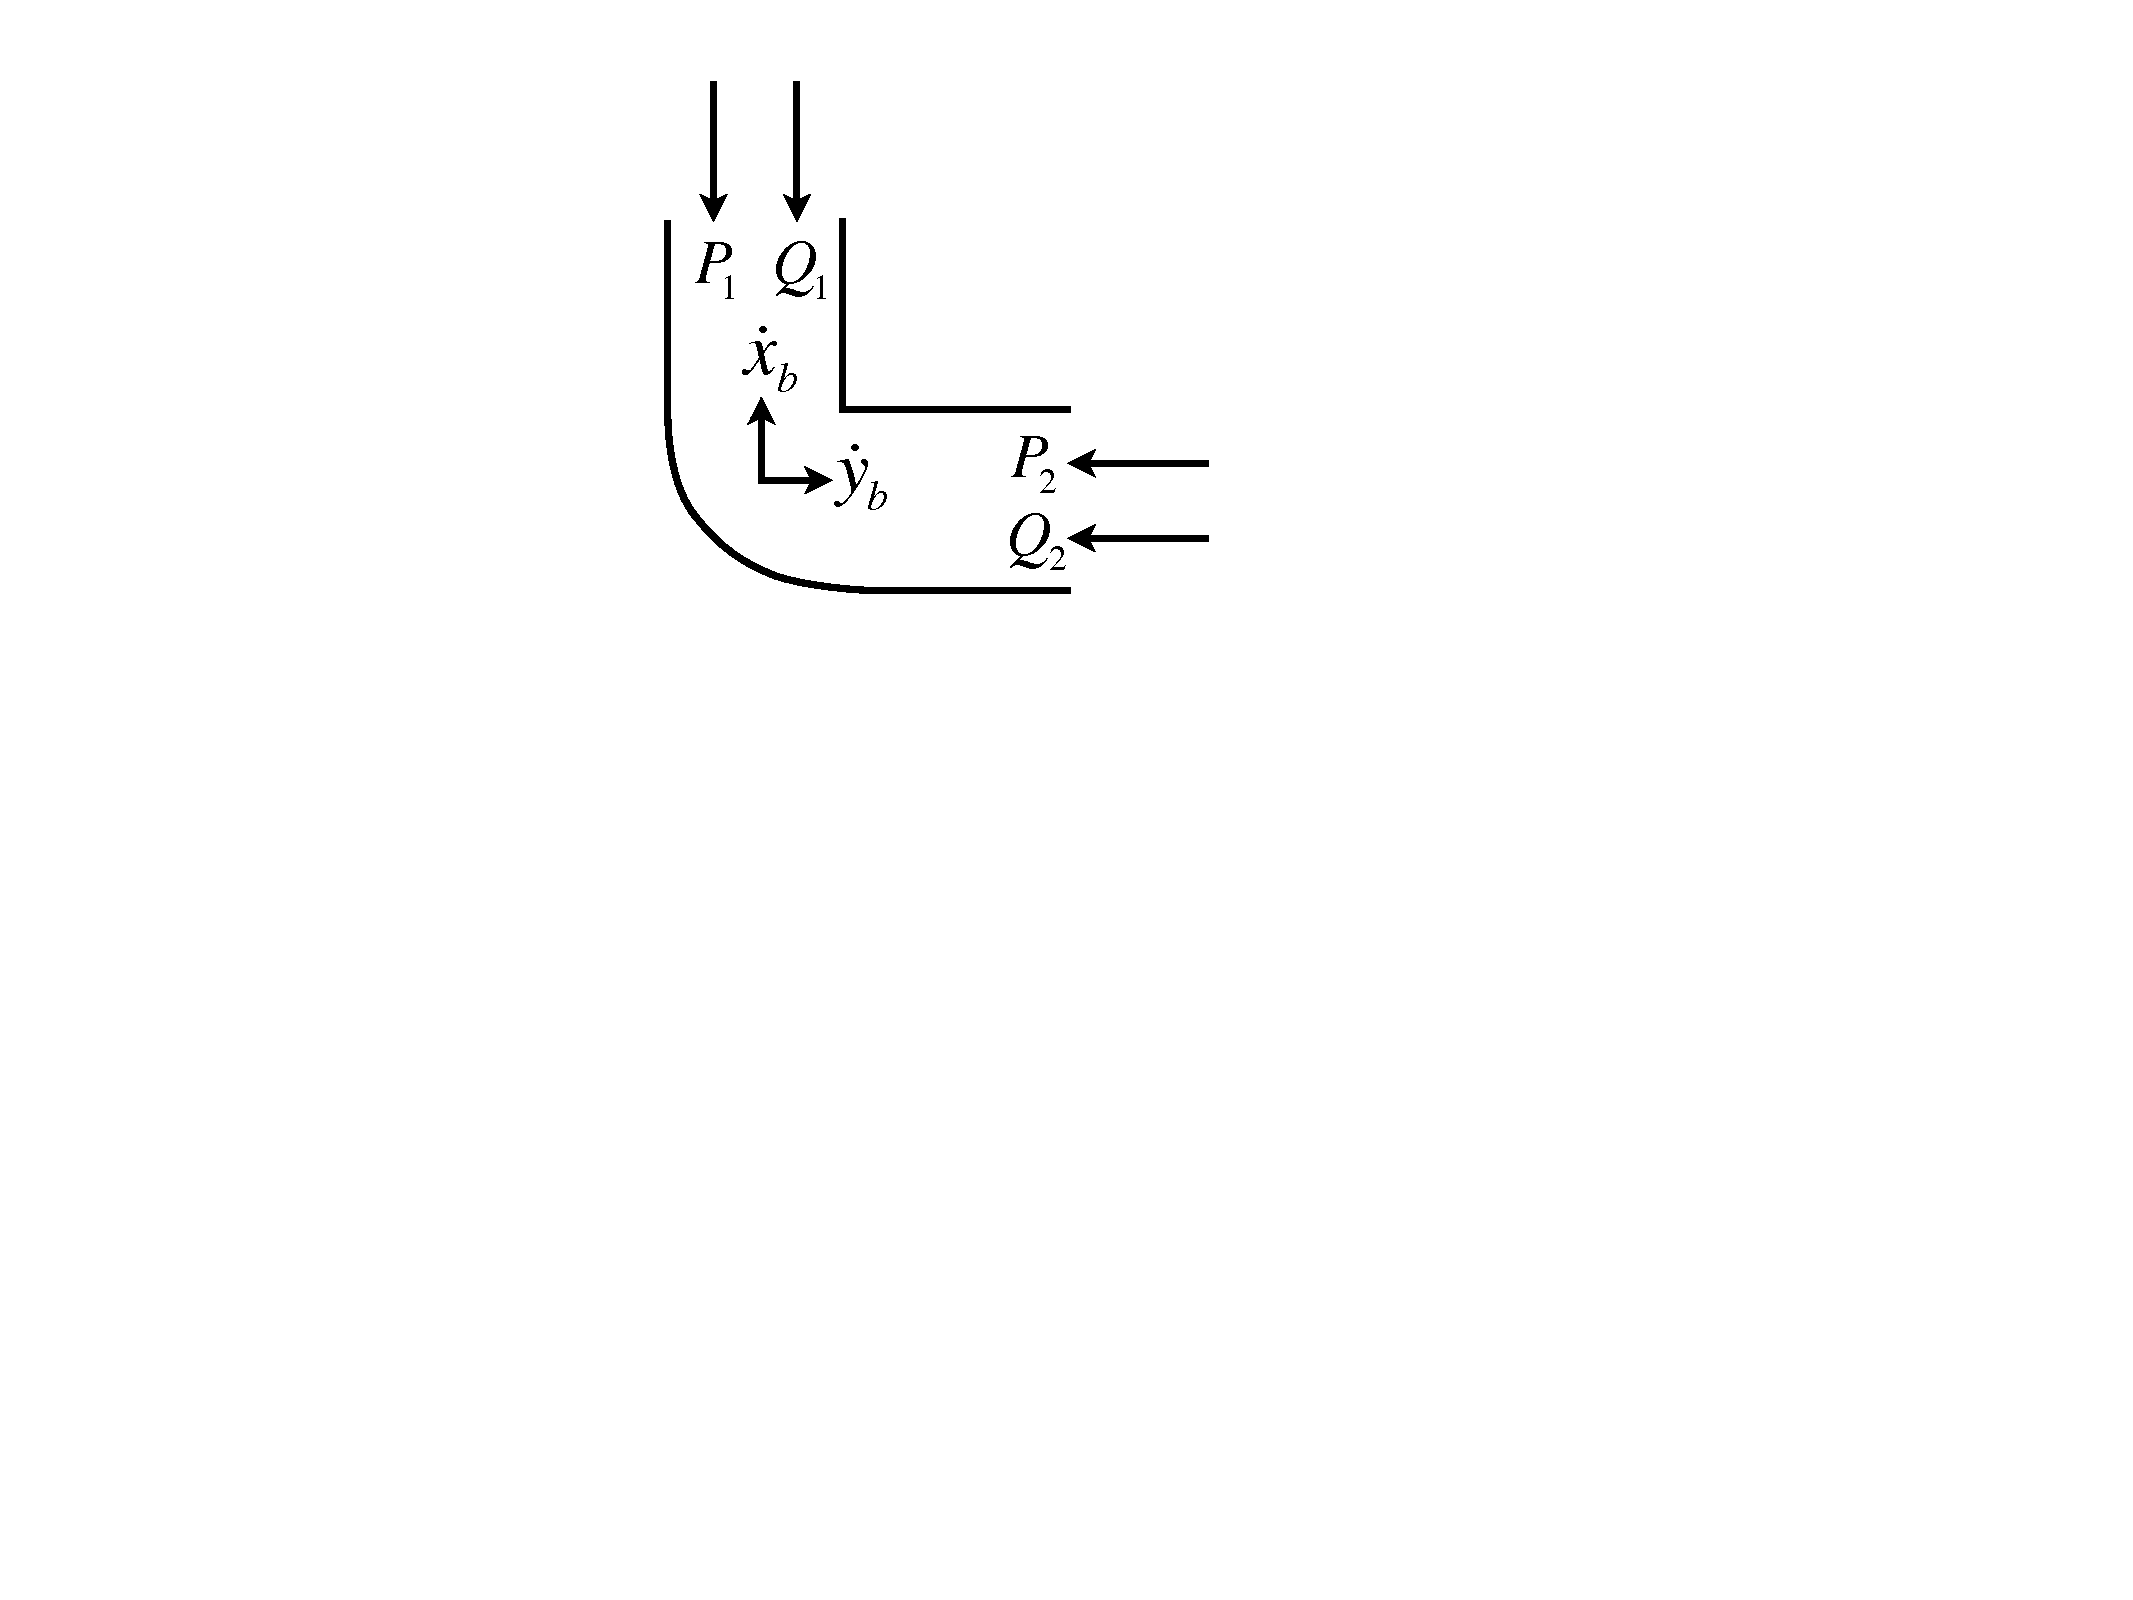
\includegraphics[width=1.7in]{Pump.pdf}
    \caption*{(f) 发动机泵}
  \end{minipage}
  \caption{液体火箭管路系统典型元件}
  \label{FeedLine-TypicalElement}
\end{figure}

分子动力学是通过统计方法来研究材料性质的计算工具,在1946年计算机发明以后立刻使得对粒子的数值模拟成为了可能。
液体推进火箭的管路系统主要由抽吸管路、多通接头、泵、泵后管路、燃烧室、推力室、蓄压器等几部分组成(如图\ref{FeedLine-TypicalElement})。分析液体火箭流体系统动特性的方法有很多,这里采用工程上常用的集中参数分析法,又称LRC等效电路分析法\cite{Dimaggio:1972, Vaage:1972, YangMing:2010}。本节主要针对包含四管发动机的推进系统展开分析。假设四管发动机系统的结构是对称的,并且流体的流动状态也是对称的,可以将四管发动机系统简化为单管发动机系统进行处理。单管发动机管路系统各元件之间脉动压力和脉动流量的传递关系如图\ref{POGO-PipeLine}所示。

\begin{figure}[!htb]
  \centering
  %%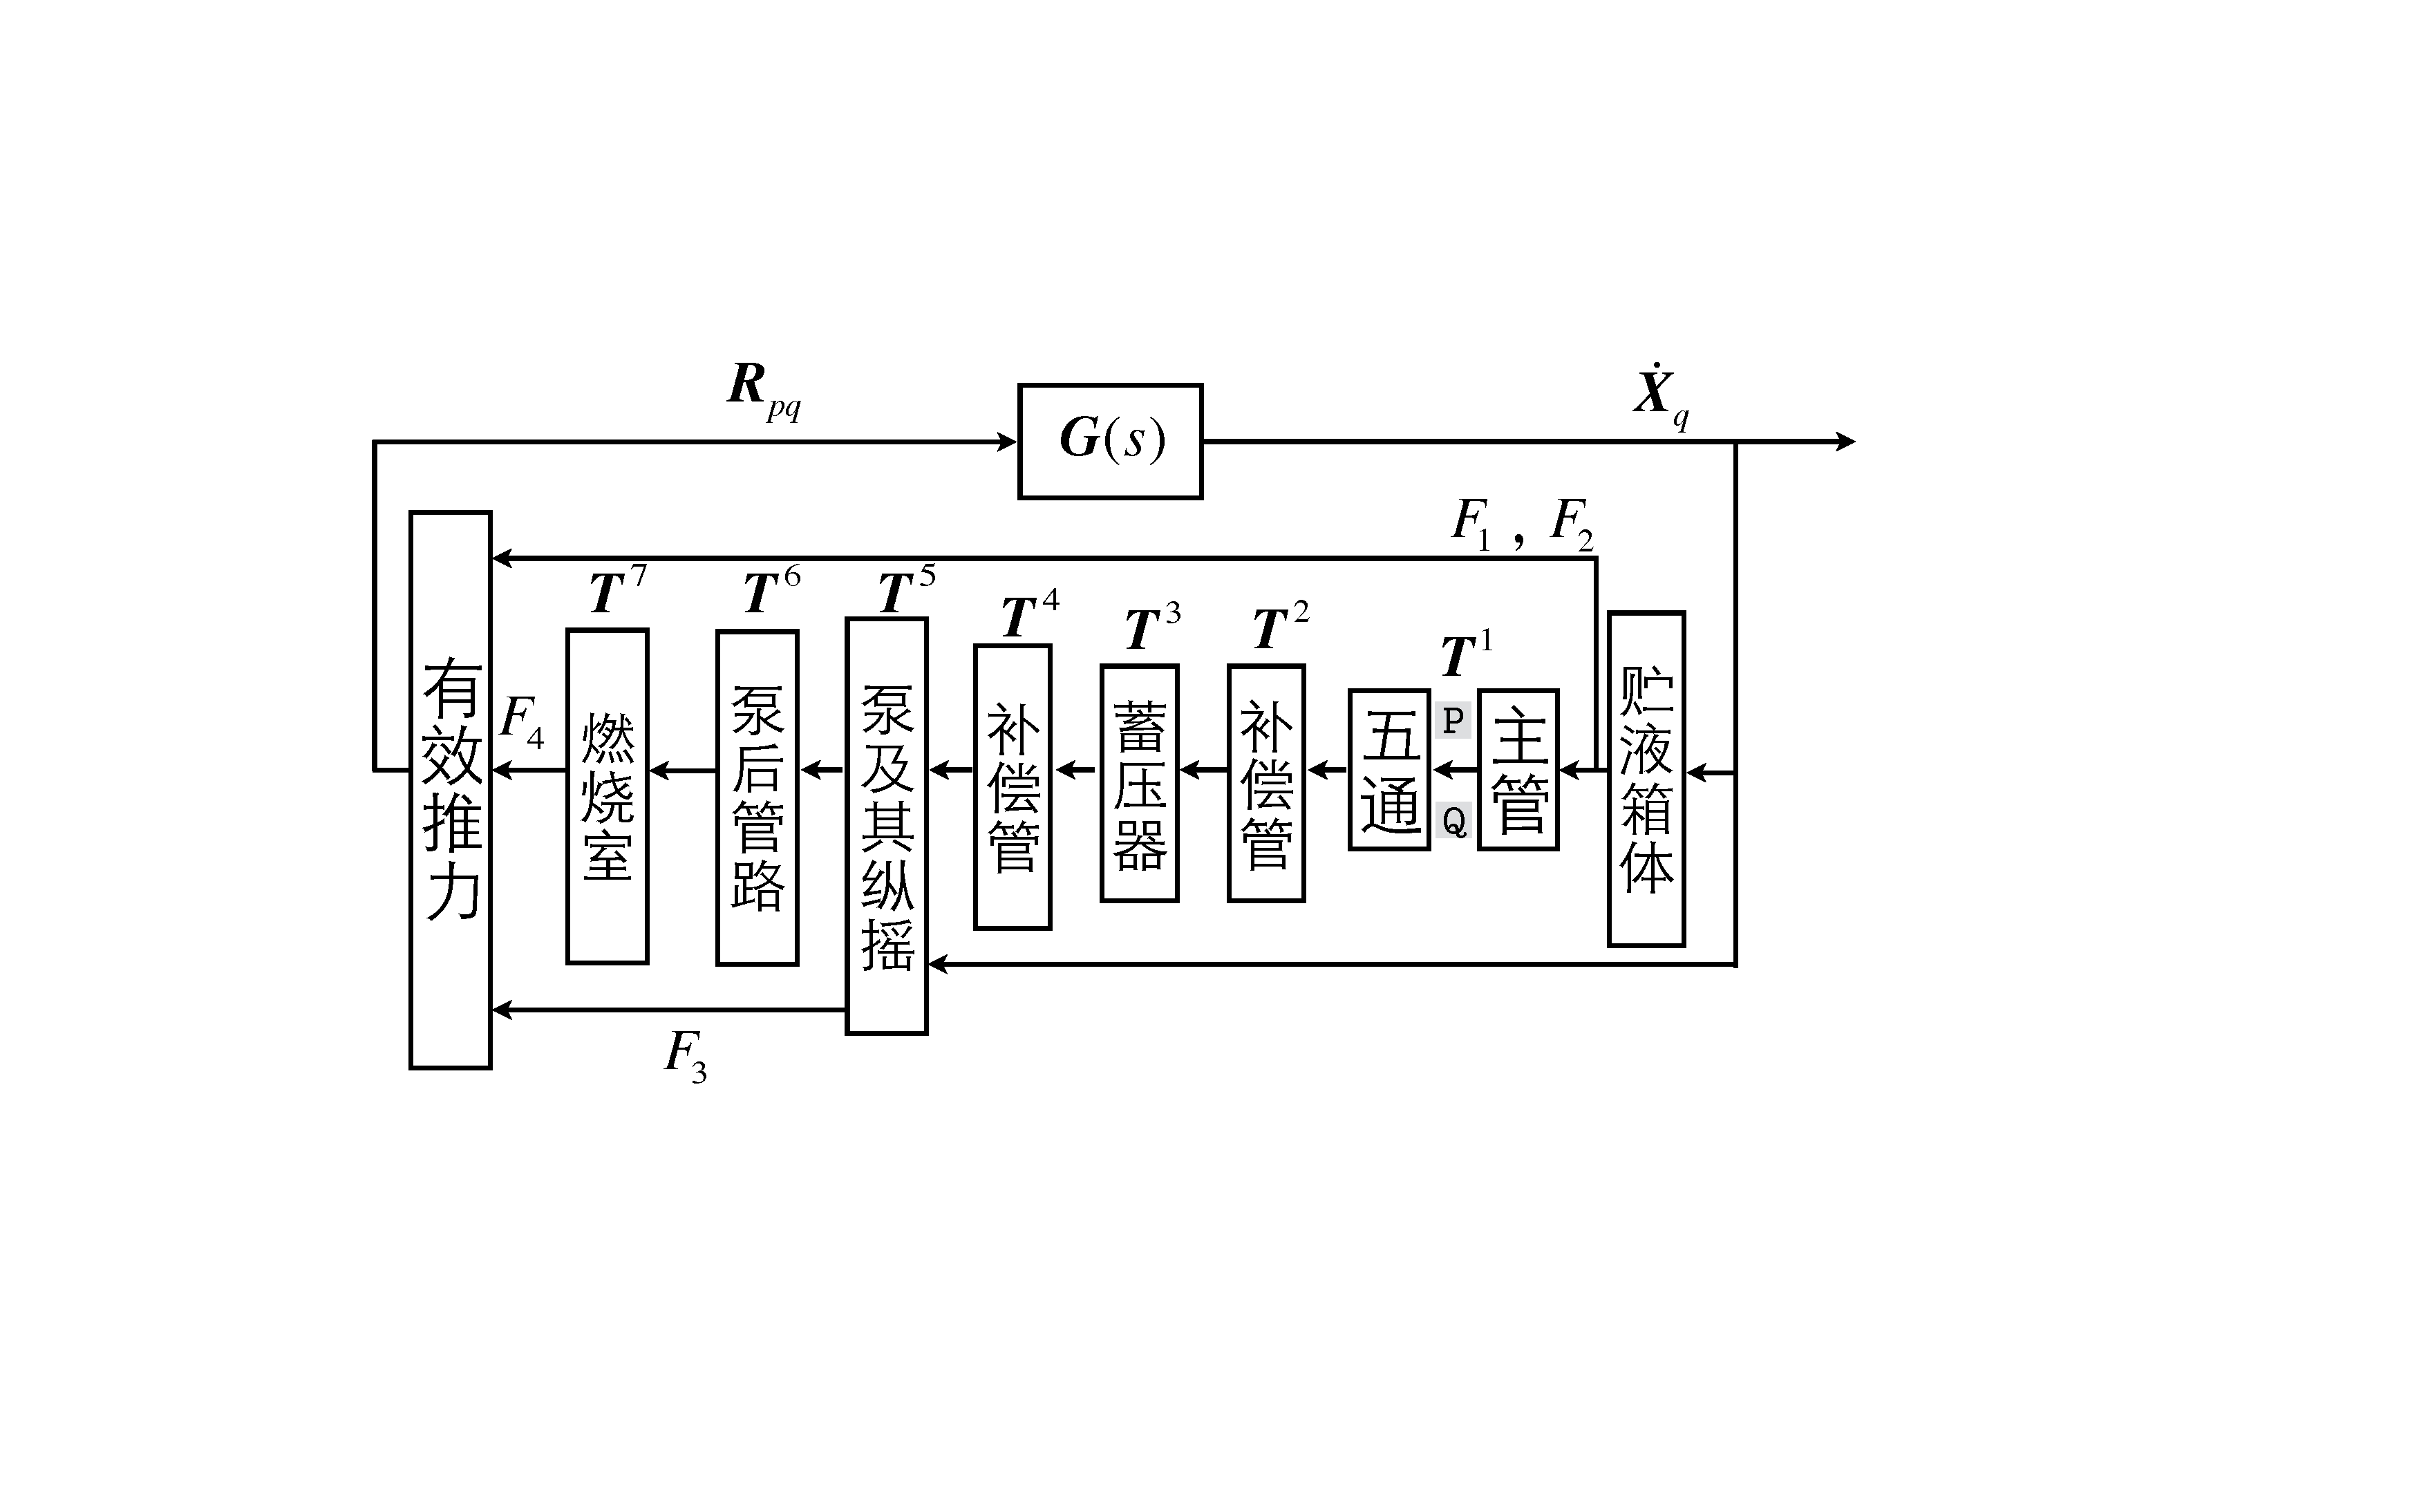
\includegraphics[width=.9\linewidth]{PipeLines.pdf}
  \caption{液体火箭管路-结构耦合系统传递关系示意图}\label{POGO-PipeLine}
\end{figure}

\begin{enumerate}[label=\textbf{\Roman*.}, align=left, leftmargin=0pt, listparindent=\parindent, itemindent=!, labelwidth=\parindent, labelsep=0pt, itemsep=1em]
  \litem{输液直管}
  由于通常情况下输液直管的直径与长度之比很小,所以在研究其低频振动时,可以不考虑管两端的复杂现象,仅考虑液体的一维流动。管中液体的扰动可以用欧拉方程和连续性方程来描述:
  \begin{align}
    \frac{\partial v}{\partial t}+{{v}_{0}}\frac{\partial v}{\partial x}+\frac{1}{\rho }\frac{\partial p}{\partial x} & =0 \nonumber \\
    \frac{\partial p}{\partial t}+{{v}_{0}}\frac{\partial p}{\partial x}+c_{0}^{2}\rho \frac{\partial v}{\partial x}  & =0
  \end{align}
  其中$v_0,c_0$为未扰动流的速度和当地声速,$p(x,t),v(x,t)$为流体的脉动压力和脉动速度。对上式进行求解,经过推导可以得到如下的输液直管上、下游脉动压力和流量之间的传递关系式:
  \begin{equation}
    \label{eq:Straight-Tube}
    \left[ \begin{matrix}
        {{P}_{2}} \\
        {{Q}_{2}} \\
      \end{matrix} \right]=\left[ \begin{matrix}
        \cosh \left( \theta  \right)                                   & {\displaystyle -\frac{Z\sinh \left( \theta  \right)}{\theta }} \\
        {\displaystyle -\frac{\theta \sinh \left( \theta  \right)}{Z}} & \cosh \left( \theta  \right)                                   \\
      \end{matrix} \right]\left[ \begin{matrix}
        {{P}_{1}} \\
        {{Q}_{1}} \\
      \end{matrix} \right]
  \end{equation}
  式中$Z=sL+R,L=\rho l/A,\tau =lc,\theta^2=s^2\tau^2Z/(sL)$,其中$l$为管路长度,$Z$为液路阻抗,$L$为液路惯性,$R$为液路阻力,$c$为当地声速,$\rho$为液体密度,$s$为拉普拉斯变量,$A$为管路截面积。

  \litem{蓄压器动力学模型}蓄压器是典型的POGO振动抑制器件,这里主要介绍目前国内外广泛应用的被动封闭式蓄压器,其简化物理模型如图\ref{FeedLine-TypicalElement}(c)所示。这种蓄压器包括了气腔和液腔,假设内部气体满足多方气体定律$P_gV_g^{\gamma}=C_g$,模拟输液直管传递关系的推导方法,可以得出其如下的传递关系:
  \begin{equation}
    \left[ \begin{matrix}
        {P_2} \\
        {Q_2} \\
      \end{matrix} \right]=\left[ \begin{matrix}
        1  & 0 \\
        -Y & 1 \\
      \end{matrix} \right]\left[ \begin{matrix}
        {P_1} \\
        {Q_1} \\
      \end{matrix} \right]
  \end{equation}
  记蓄压器阻抗为$Z$、导纳为$Y$
  \begin{align}
    Z & =\frac{s^2CL+sCR+1}{sC} \nonumber                                                         \\
    Y & =\frac{1}{Z}=\frac{s}{\displaystyle L\left(s^2+2\zeta\omega s+\omega^2 \right)} \nonumber
  \end{align}
  其中$\omega=\sqrt{1/CL},\zeta=CR\omega/2$,$C$为蓄压器柔度,$R$和$L$意义同上。
\end{enumerate}

至此,可以利用上述管段元件的传递关系进行液体火箭管路系统的总体传递矩阵组装(矩阵记号参考图\ref{POGO-PipeLine})
\begin{equation}
  \boldsymbol{\mathbb{T}}=\boldsymbol{T}^6\boldsymbol{T}^5\boldsymbol{T}^4\boldsymbol{T}^3\boldsymbol{T}^2\boldsymbol{T}^1=\left[ \begin{matrix}
      {T}_{11} & {T}_{12} \\
      {T}_{21} & {T}_{22} \\
    \end{matrix} \right],\;
  \boldsymbol{T}^s=\boldsymbol{T}^6 \left[
    \begin{matrix}
      -A_{L1}^{(5)}Z_{L1}^{(5)} \\
      A_{L1}^{(5)}              \\
    \end{matrix} \right] = \left[ \begin{matrix}
      {T}_{1}^s \\
      {T}_{2}^s \\
    \end{matrix} \right]
\end{equation}
考虑管路系统入口处脉动压力和脉动流量与箱底振动速度之间的关系:
\begin{equation}
  \label{eq:Inlet-Boundary-Condition}
  P_{L1}^{(1)}=s\rho{h}_T\left(1-\frac{A_{L1}^{(1)}}{A_T}\right){\dot{x}_T}(s)- \frac{s\rho{h_T}Q_{L1}^{(1)}}{A_T}
\end{equation}
其中,符号下标${}_{L1},{}_{L2}$用于区分管路参数描述位置(入口或出口),数字上标${}^{(n)}$表示该参数描述第$n$段管路元件, $h_T$为贮箱液面高度,$A_{L1}^{(1)}, A_T$分别表示与贮箱底部相连管路的截面积和贮箱截面积,$\dot{x}_T$表示箱底扰动速度。

结合发动机燃烧室内的压力上下游平衡关系$P_{L1}^{(7)}=P_{L2}^{(6)}$,经过一系列换算,最终可以得到管路系统初始脉动压力$P_{L1}^{(1)}$和脉动流量$Q_{L1}^{(1)}$与箱底扰动速度$\dot{x}_T$和泵位置扰动速度$\dot{x}_{L1}^{(5)}$之间的传递关系:
\begin{align}
  \label{eq:Total-Transfer}
  Q_{L1}^{(1)}= & \frac{\left( {T}_{1}^{s}-Z_{L1}^{(7)} {T}_{2}^{s} \right)\dot{x}_{L1}^{(5)}(s)- s{\rho}{h_T}\left( 1- {\displaystyle \frac{A_{L1}^{(1)}}{A_T}} \right) \left( Z_{L1}^{(7)} {T}_{21}- {T}_{11} \right) {\dot{x}_T(s)} } {Z_{L1}^{(7)} {T}_{22}- {T}_{12}- {\displaystyle \frac{s\rho h_T}{A_T}} \left( Z_{L1}^{(7)} {T}_{21}- {T}_{11} \right)} \nonumber \\
  %%%
  P_{L1}^{(1)}=% 
                & -\frac{s\rho{h_T}}{A_T} \left[
  \frac{\left( {T}_{1}^{s}-Z_{L1}^{(7)} {T}_{2}^{s} \right)\dot{x}_{L1}^{(5)}(s)- s{\rho}{h_T}\left( 1- { \frac{A_{L1}^{(1)}}{A_T}} \right) \left( Z_{L1}^{(7)} {T}_{21}- {T}_{11} \right) {\dot{x}_T(s)} } {Z_{L1}^{(7)} {T}_{22}- {T}_{12}- { \frac{s\rho h_T}{A_T}} \left( Z_{L1}^{(7)} {T}_{21}- {T}_{11} \right)}
  \right] \nonumber                                                                                                                                                                                                                                                                                                                                                        \\
                & + s\rho{h}_T \left(1- \frac{A_{L1}^{(1)}}{A_T}\right){\dot{x}_T}(s)
\end{align}

通常,作用在液体火箭上的典型外力主要包括了以下几类:\label{Page:Typical-Feedback-Force}
\begin{enumerate}[leftmargin=\parindent, align=parleft, labelindent=0pt, labelwidth=*]
  \item 贮箱底开口处相对脉动流出量引起贮箱液体质心脉动对结构作用力。
        \begin{equation}
          F_1=\rho h_Ts \left[ Q_{L1}^{(1)}+ A_{L1}^{(1)}\dot{x}_T(s) \right]
        \end{equation}
  \item 贮箱底开口处的脉动压力对结构作用力。
        \begin{equation}
          F_2=A_{L1}^{(1)}P_{L1}^{(1)}
        \end{equation}
  \item 泵前后压力动量变化对结构作用力。
        \begin{equation}
          F_3=N\left[ -A_{L1}^{(4)}P_{L1}^{(5)}- \rho Q_s \left( \frac{2Q_{L1}^{(5)}}{A_{L1}^{(4)}}+ \dot{x}_{L1}^{(5)}(s) \right)\right]
        \end{equation}
  \item 发动机燃烧室脉动压力引起脉动推力。
        \begin{equation}
          F_4=NA_{th}C_f P_{L2}^{(7)}
        \end{equation}
\end{enumerate}
其中,$A_{L1}^{(4)}$表示泵上游入口处截面积,$Q_s$表示泵的稳态体积流,$N$表示发动机台数,$A_{th}$为发动机喉部截面积,$C_f$为有效推力系数。

利用公式\eqref{eq:Total-Transfer},可以把管路推进系统作用到结构上的反馈力表示为:
\begin{equation}
  \label{eq:Feedback-Force-Transfer}
  \boldsymbol{F}_p(s)=\left[ \begin{matrix}
      F_1(s) \\
      F_2(s) \\
      F_3(s) \\
      F_4(s) \\
    \end{matrix} \right]  \triangleq \boldsymbol{R}_{pq}(s)\left[ \begin{matrix}
      \dot{x}_T(s)          \\
      \dot{x}_{L1}^{(5)}(s) \\
    \end{matrix} \right] \triangleq \boldsymbol{R}_{pq}(s)\boldsymbol{\dot{X}}_q(s)
\end{equation}
矩阵$\boldsymbol{R}_{pq}(s)$代表了箭体振动速度$\boldsymbol{\dot{X}}_q(s)$与推进系统反馈力$\boldsymbol{F}_p(s)$之间的传递关系。可以看出,该速度阻抗矩阵形式复杂,且包含了难以处理的超越函数。

\section{液体火箭结构系统集中参数模型}
\label{sec:Lumped-Rocket-Structural-System}
\begin{figure}[!htb]
  \centering
  %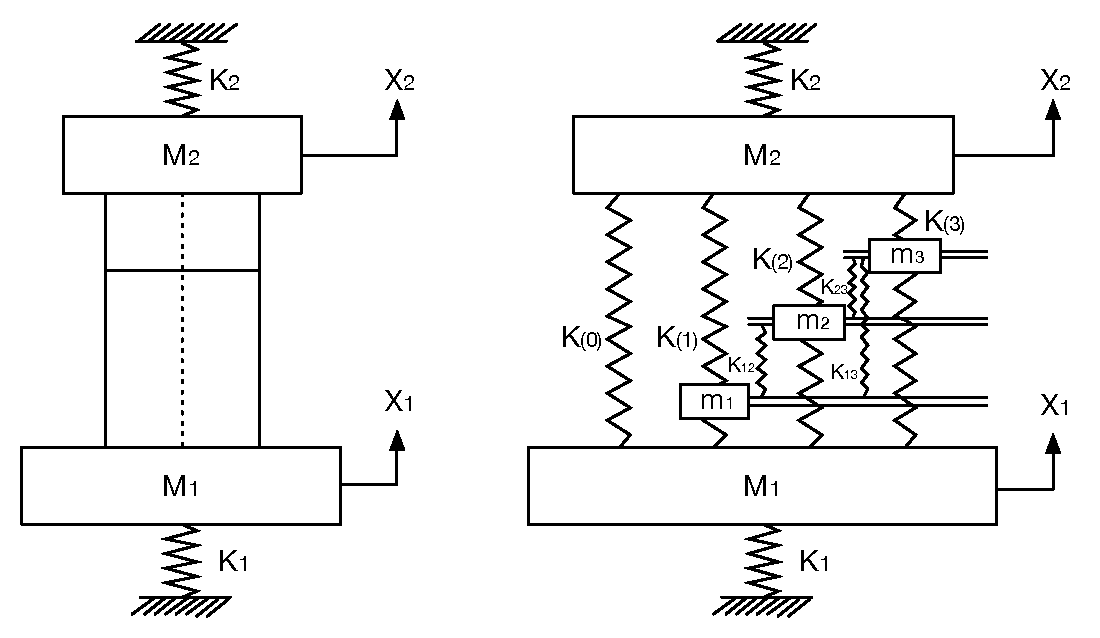
\includegraphics[width=.8\linewidth]{Lumped-Mass-Spring-Glaser}
  \caption{液体贮箱集中参数Glaser弹簧-质量模型}\label{Lumped-Mass-Spring-Glaser}
\end{figure}

\begin{figure}[p]
  \centering
  \centerline{%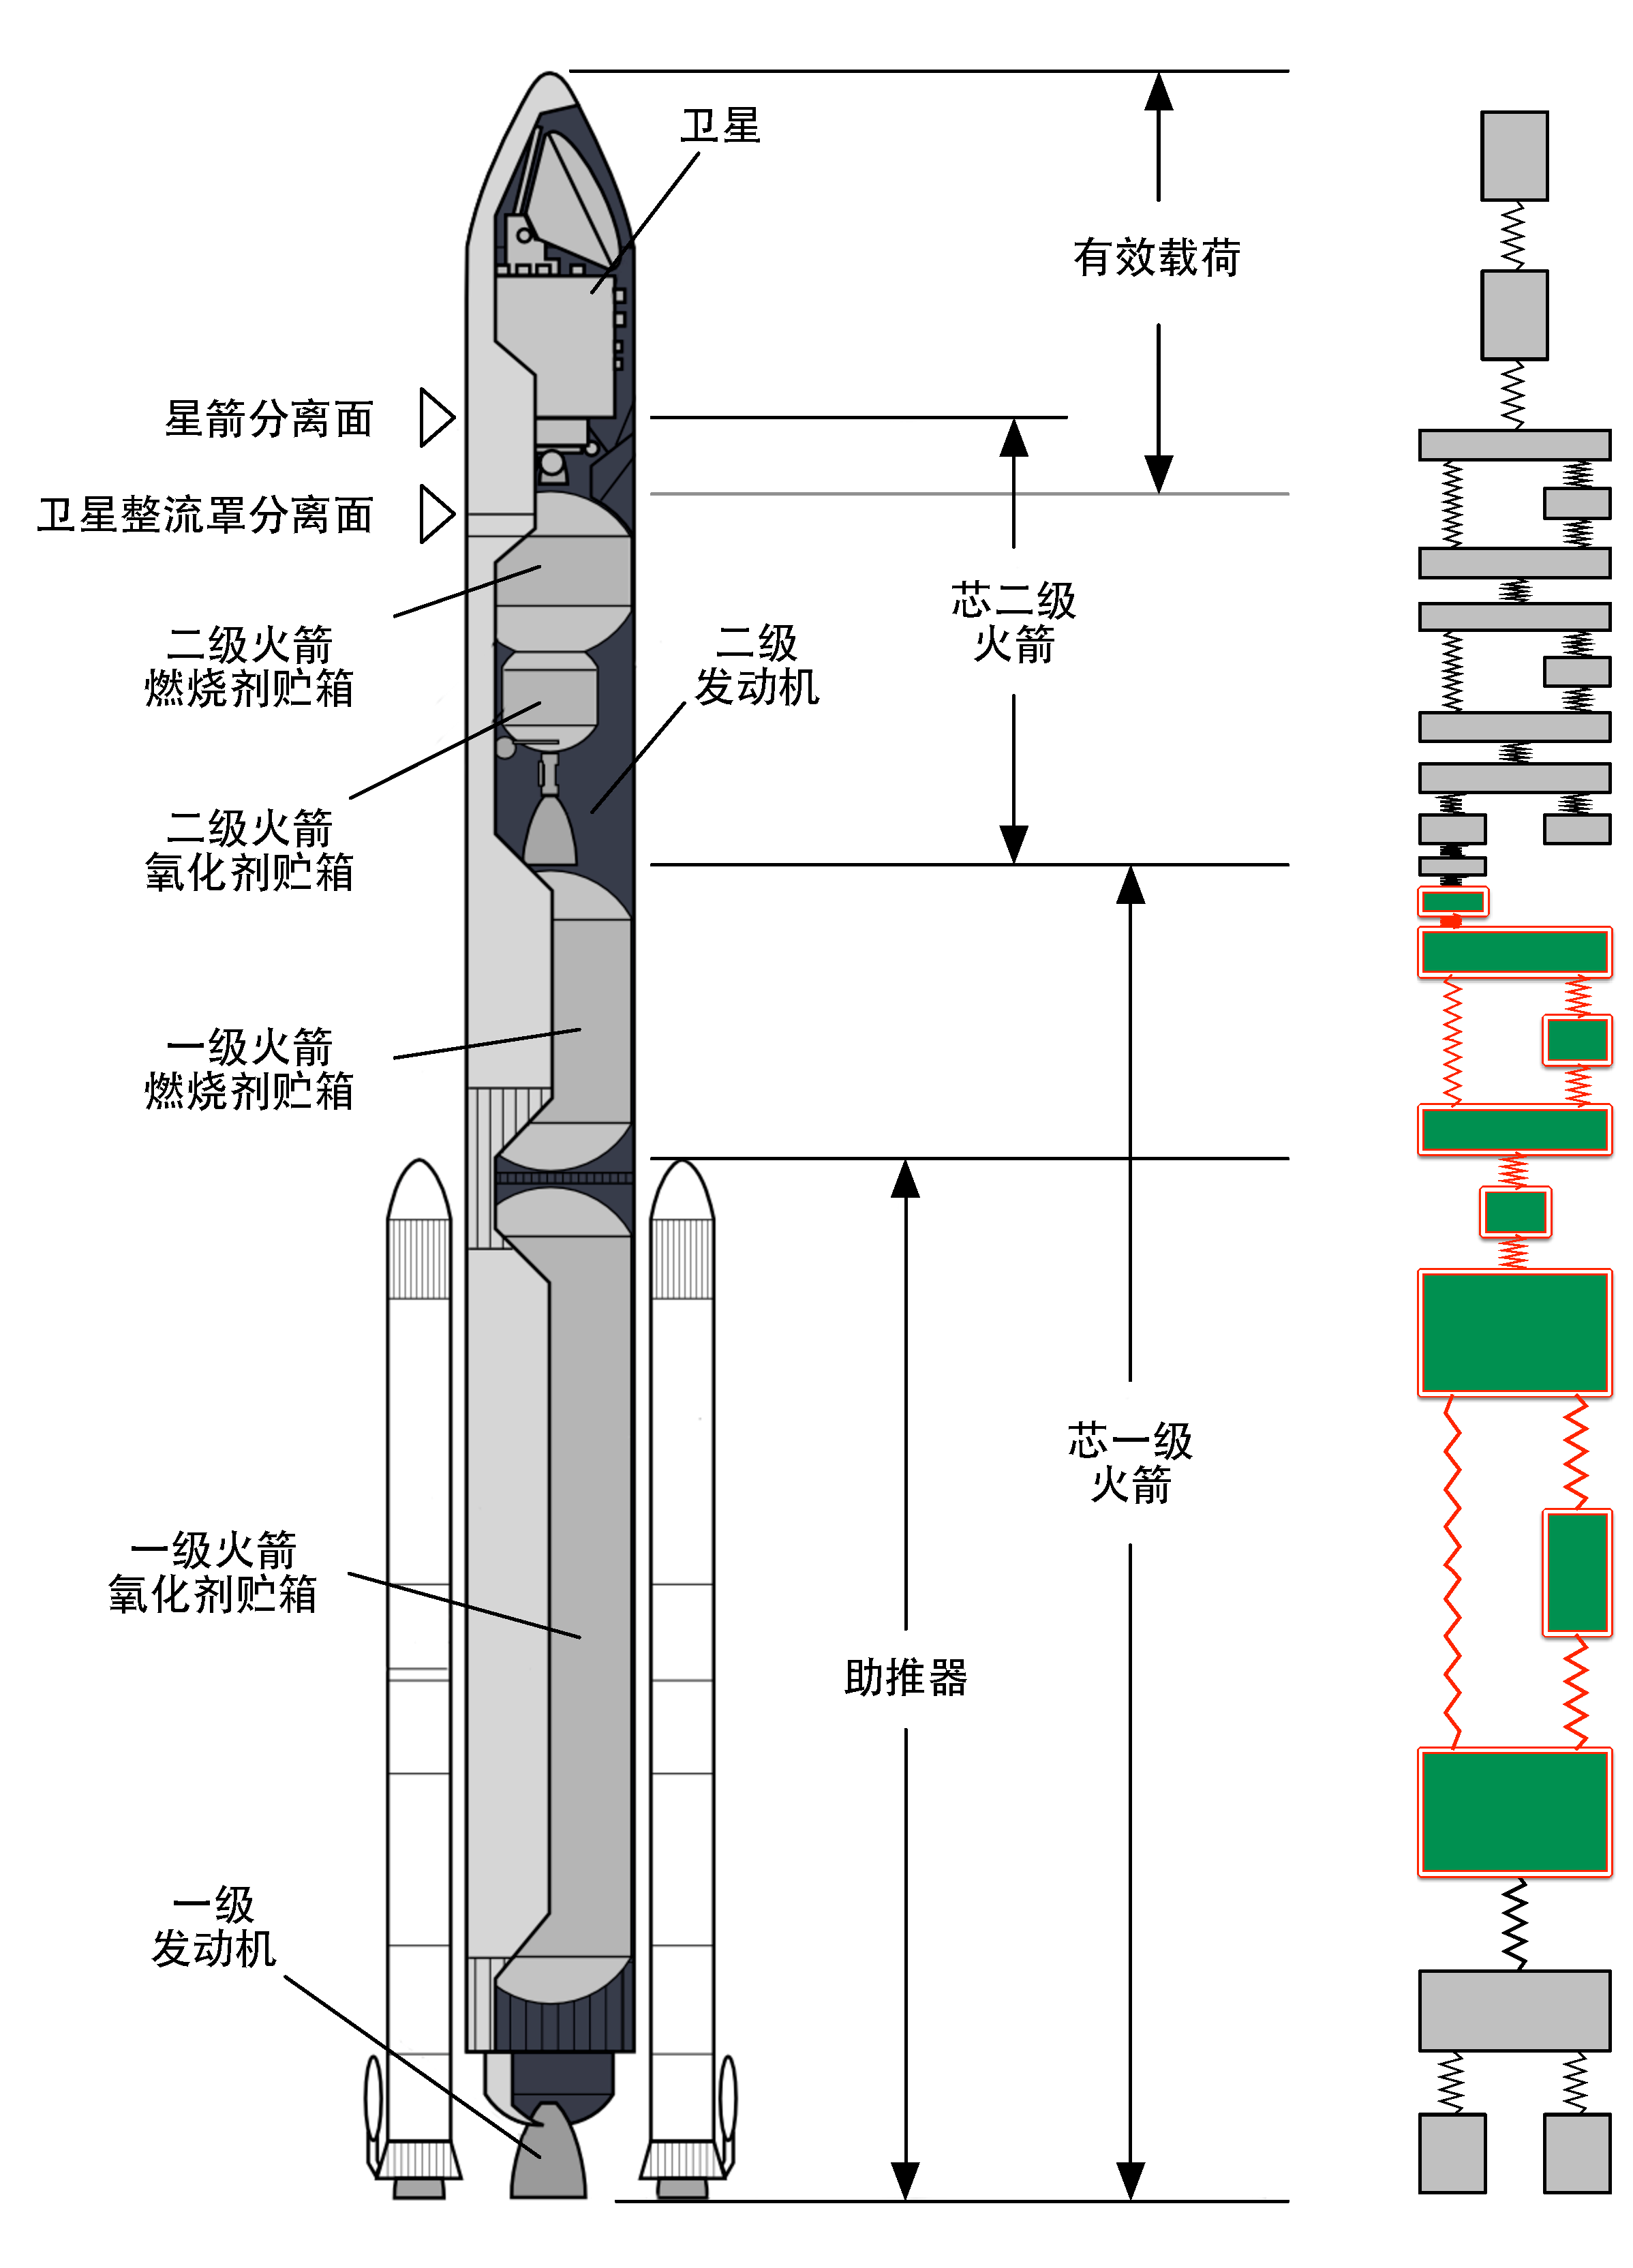
\includegraphics[width=.95\linewidth]{Whole-Rocket-Model}
  }
  \caption{液体火箭全箭集中质量模型}\label{Whole-Rocket-Model}
\end{figure}

\section{耦合系统稳定性分析方法}
传统的液体火箭POGO稳定性分析方法主要分为了矩阵法、单传法和临界阻尼法\cite{Wang-Qizheng:1999}等几类。从现代控制理论的角度出发\cite{Ogata:2009},这些方法从本质上看都是通过求解系统特征值来判断系统是否稳定:耦合系统特征值出现正实部则系统不稳定,若特征值实部全为负数则系统稳定。其中,矩阵法可分为闭环分析法和开环分析法,是传统POGO稳定性分析方法中最复杂、精度最高的。其余两种方法虽然计算过程较为简单,但由于计算结果精度较差,所以研究者们逐渐的将目光转向了更能满足目前工况计算要求的新型稳定性分析方法。本节将引入一种基于矩阵法的新型POGO稳定性快速求解方法。

根据公式\eqref{eq:Feedback-Force-Transfer}和\eqref{eq:Structure-Dynamic-Freq},可以把耦合系统的频域特征方程表示为:
\begin{equation}
  \label{eq:Coupled-System-Transfer-TMP}
  \left[s^2 \boldsymbol{M}_s+ s(\boldsymbol{C}_s+\boldsymbol{\dot{M}}_s)+ \boldsymbol{K}_s \right]\boldsymbol{X}_s(s)=\boldsymbol{F}_s(s)+ \boldsymbol{L}_{sp} \boldsymbol{R}_{pq}(s)\boldsymbol{\dot{X}}_q(s)
\end{equation}
若引入转换结构系统速度反馈节点位置的布尔矩阵,
\begin{displaymath}
  \boldsymbol{x}_q(t)=
  \left[ \begin{matrix}
      {x}_T(t) & {x}_{L1}^{(5)}(t)
    \end{matrix} \right]^{\ut}=
  \boldsymbol{L}_{qs} \boldsymbol{x}_s(t)
\end{displaymath}
可将公式\eqref{eq:Coupled-System-Transfer-TMP}改写为:
\begin{equation}
  \label{eq:Coupled-System-Transfer}
  \left[s^2 \boldsymbol{M}_s+ s\left(\boldsymbol{C}_s+\boldsymbol{\dot{M}}_s
    -\boldsymbol{L}_{sp} \boldsymbol{R}_{pq}(s)\boldsymbol{L}_{qs}\right)+ \boldsymbol{K}_s \right]\boldsymbol{X}_s(s)=\boldsymbol{F}_s(s)
\end{equation}
耦合系统稳定的准则是如下代数方程根的实部均不大于零:
\begin{equation}
  \label{eq:Coupled-Transfer-Det}
  \Psi (s) \triangleq \det
  \left[s^2 \boldsymbol{M}_s+ s\left(\boldsymbol{C}_s+\boldsymbol{\dot{M}}_s
    -\boldsymbol{L}_{sp} \boldsymbol{R}_{pq}(s)\boldsymbol{L}_{qs}\right)+ \boldsymbol{K}_s \right]\boldsymbol{X}_s(s)=0
\end{equation}

\subsection{反馈力传递函数的有理分式拟合方法}
从公式\eqref{eq:Coupled-Transfer-Det}的形式可以看出,耦合系统特征值问题的求解难点主要缘于阻抗函数$\boldsymbol{R}_{pq}(s)$的形式较为复杂。所以本节主要研究如何将其进行合理的等效变换,将包含了诸如双曲函数形式的管路系统反馈力传递函数转化为便于与液体火箭结构系统进行耦合分析的有理分式形式。

如果只考虑阻抗矩阵$\boldsymbol{R}_{pq}(s)$的单个元素,可以利用有理分式将此单输入单输出(SISO)传递函数在频域拟合为如下标准形式\cite{Gustavsen:1999, Zeng:2006}:
\begin{equation}
  \label{eq:Standard-SISO-Freq}
  T(\jmath\omega)=\jmath\omega M_0+ D_0+ \sum_{k=1}^{n}\frac{C_k}{\jmath\omega-A_k}+ \sum_{k=1}^{n}\frac{\bar{C}_k}{\jmath\omega- \bar{A}_k}+ \sum_{j=1}^{m} \frac{B_j}{\jmath\omega -R_j}
\end{equation}

其中$\jmath=\sqrt{-1}$,$A_k, R_j$为已知的极点,$M_0, D_0, C_k, B_j$为待定系数,符号$\bar{}$表示对应变量的共轭。值得注意的是,此处考虑了有理分式中包含成对出现的共轭极点、纯实数极点、直流分量和一次项的广义情况,实际拟合过程可能只需要保留其中的部分项。

根据离散的传递函数数据,可以在$n_f$个频率点上建立如下方程:
\begin{equation}
  \label{eq:Discrete-Standard-Transfer}
  T(\jmath\omega_f)=\jmath\omega_f M_0+ D_0+ \sum_{k=1}^{n}\frac{C_k}{\jmath\omega_f-A_k}+ \sum_{k=1}^{n}\frac{\bar{C}_k}{\jmath\omega_f- \bar{A}_k}+ \sum_{j=1}^{m} \frac{B_j}{\jmath\omega_f -R_j}
\end{equation}
记
\begin{align}
   & \boldsymbol{m}_1(\omega_f)=\left[ \begin{matrix}
      \jmath\omega_f & 1
    \end{matrix} \right] \nonumber \\
   & \boldsymbol{m}_2(\omega_f)=\left[ \begin{matrix}
      \displaystyle{\frac{1}{\jmath \omega_f-A_1}} & \cdots & \displaystyle{\frac{1}{\jmath \omega_f-A_n}} \\
    \end{matrix} \right] \nonumber \\
   & \boldsymbol{m}_3(\omega_f)=\left[ \begin{matrix}
      \displaystyle{\frac{1}{\jmath \omega_f-\bar{A}_1}} & \cdots & \displaystyle{\frac{1}{\jmath \omega_f-\bar{A}_n}} \\
    \end{matrix} \right]           \\
   & \boldsymbol{m}_4(\omega_f)=\left[ \begin{matrix}
      \displaystyle{\frac{1}{\jmath \omega_f-R_1}} & \cdots & \displaystyle{\frac{1}{\jmath \omega_f-R_m}} \\
    \end{matrix} \right] \nonumber \\
   & \boldsymbol{C}=\left[ \begin{matrix}
      C_1 & \cdots & C_n
    \end{matrix} \right]^{\ut} \nonumber       \\
   & \boldsymbol{B}=\left[ \begin{matrix}
      B_1 & \cdots & B_m
    \end{matrix} \right]^{\ut} \nonumber
\end{align}
可以将公式\eqref{eq:Discrete-Standard-Transfer}改写为:
\begin{equation}
  T(\jmath \omega_f)=\boldsymbol{m}_1(\omega_f)\left[
    \begin{matrix}
      M_0 \\
      D_0 \\
    \end{matrix} \right] + \boldsymbol{m}_2(\omega_f)\boldsymbol{C} + \boldsymbol{m}_3\boldsymbol{\bar{C}} +\boldsymbol{m}_4(\omega_f)\boldsymbol{B}
\end{equation}
将上式进行实部和虚部分离,方程变为
\begin{equation}
  \label{eq:SISO-Least-Square}
  \left[ \begin{matrix}
      T'(\omega_f)  \\
      T''(\omega_f) \\
    \end{matrix} \right]=\left[ \begin{matrix}
      \boldsymbol{m}'_1(\omega_f)                                & \boldsymbol{m}''_1(\omega_f)                               \\
      \boldsymbol{m}'_2(\omega_f)+ \boldsymbol{m}'_3(\omega_f)   & \boldsymbol{m}''_2(\omega_f)+ \boldsymbol{m}''_3(\omega_f) \\
      \boldsymbol{m}''_3(\omega_f)- \boldsymbol{m}''_2(\omega_f) & \boldsymbol{m}'_2(\omega_f)-\boldsymbol{m}'_3(\omega_f)    \\
      \boldsymbol{m}'_4(\omega_f)                                & \boldsymbol{m}''_4(\omega_f)                               \\
      -\boldsymbol{m}''_4(\omega_f)                              & \boldsymbol{m}'_4(\omega_f)
    \end{matrix} \right]^{\ut} \left[ \begin{matrix}
      M_0              \\
      D_0              \\
      \boldsymbol{C}'  \\
      \boldsymbol{C}'' \\
      \boldsymbol{B}'  \\
      \boldsymbol{B}'' \\
    \end{matrix} \right]
\end{equation}
其中,复数变量的记号约定如下:
\begin{equation}
  \Re(T)=T',\quad\Im(T)=T''
\end{equation}
利用最小二乘法\cite{Bjorck:1996},可以根据公式\eqref{eq:SISO-Least-Square}求解出有理分式\eqref{eq:Standard-SISO-Freq}中的各项待定系数。此外,如果发现拟合结果在某些重要频率范围内的精度达不到标的要求,还可以利用加权的最小二乘法\cite{Strutz:2011}对求解过程进行适当优化。

对于POGO研究中所涉及到的多输入多输出(MIMO)系统,可以利用上述方法对于阻抗矩阵$\boldsymbol{R}_{pq}(s)$中的各个分量进行分别拟合。值得注意的是,根据通过理论推导可以得知:管路系统反馈力传递矩阵中各个分量的极点是相同的,所以在对传递函数进行最小二乘法拟合之前,只需选其任意一个分量进行极点探测即可。如果在极点探测的过程中出现了由于数值误差或者拟合精度设置不统一等因素导致的极点不一致情况,工程上也可以将分别拟合得到的极点进行平均化处理。至于有理多项式拟合应采用多少极点,可以先解析的绘制出阻抗矩阵$\boldsymbol{R}_{pq}(s)$各分量的传递函数图形,根据曲线峰值的数目进行多项式项数的预估,然后根据具体的拟合结果进行拟合迭代次数和极点个数等参数的微调,最终得出合理的拟合结果。

\begin{figure}[p]
  \centering
  %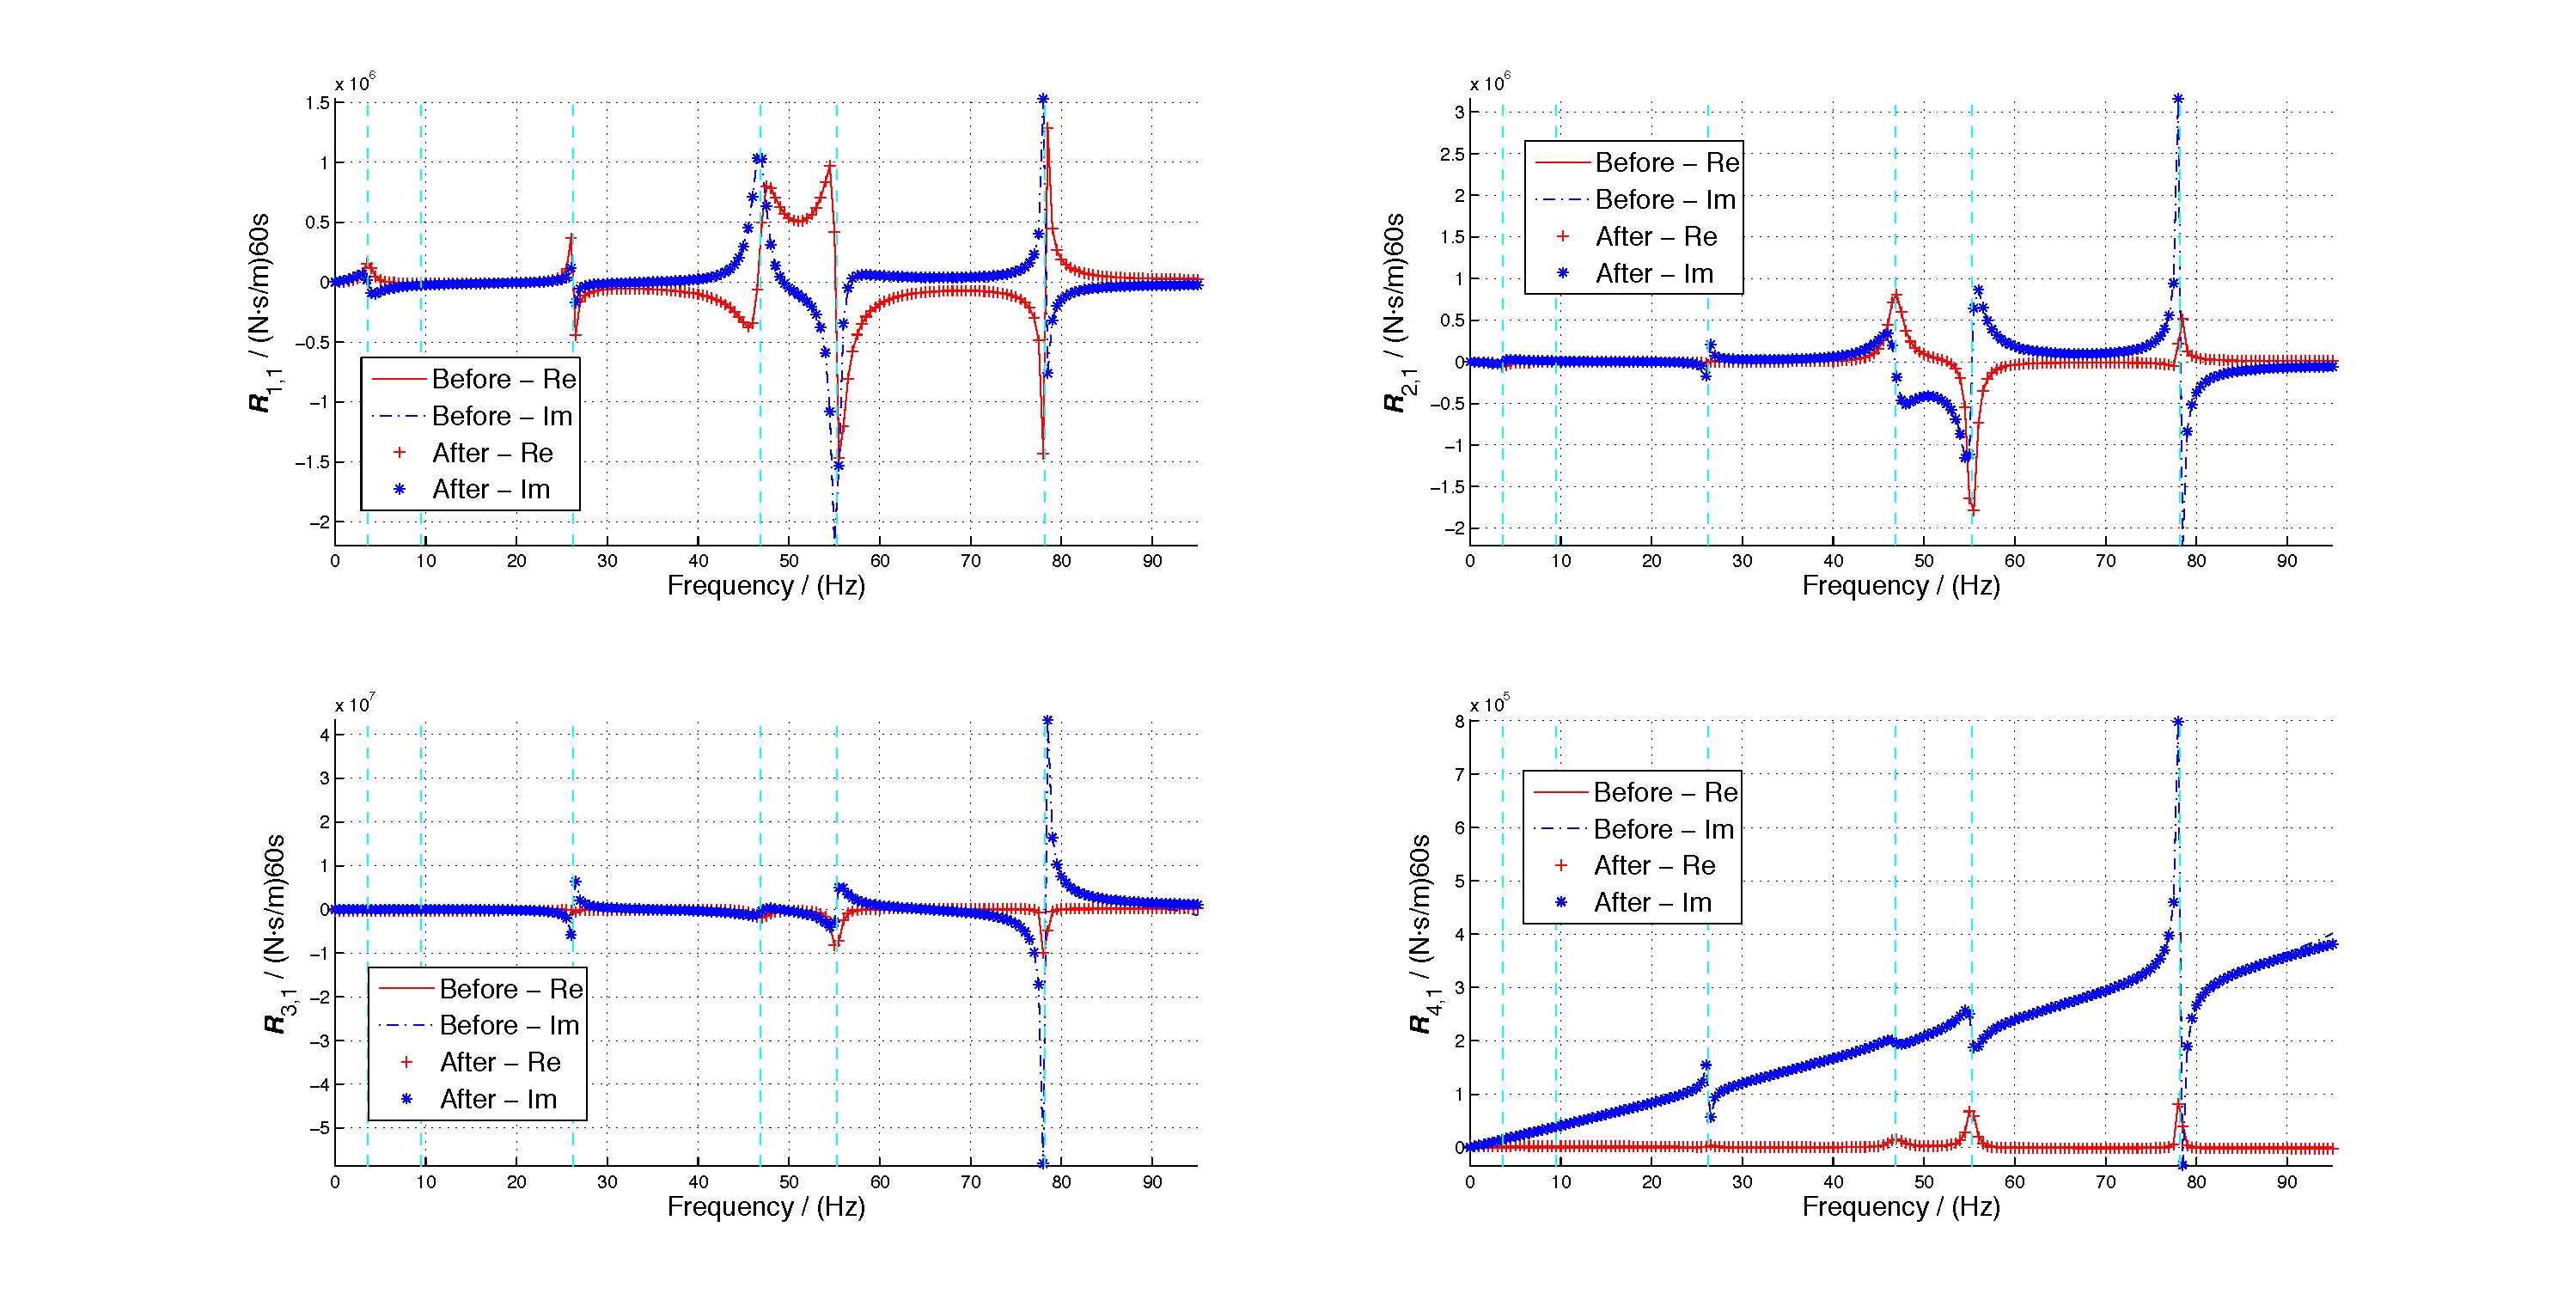
\includegraphics[trim={4.5cm 0cm 4.5cm 0cm}, clip=true, width=\linewidth]{Fitted-Transfer-01.pdf}
  \caption{管路系统反馈力有理分式拟合前后对比曲线(a):$\boldsymbol{R}_{11}-\boldsymbol{R}_{41}$}
  \label{Rational-Fitted-VS-01}
  \vspace{1.2em}
  %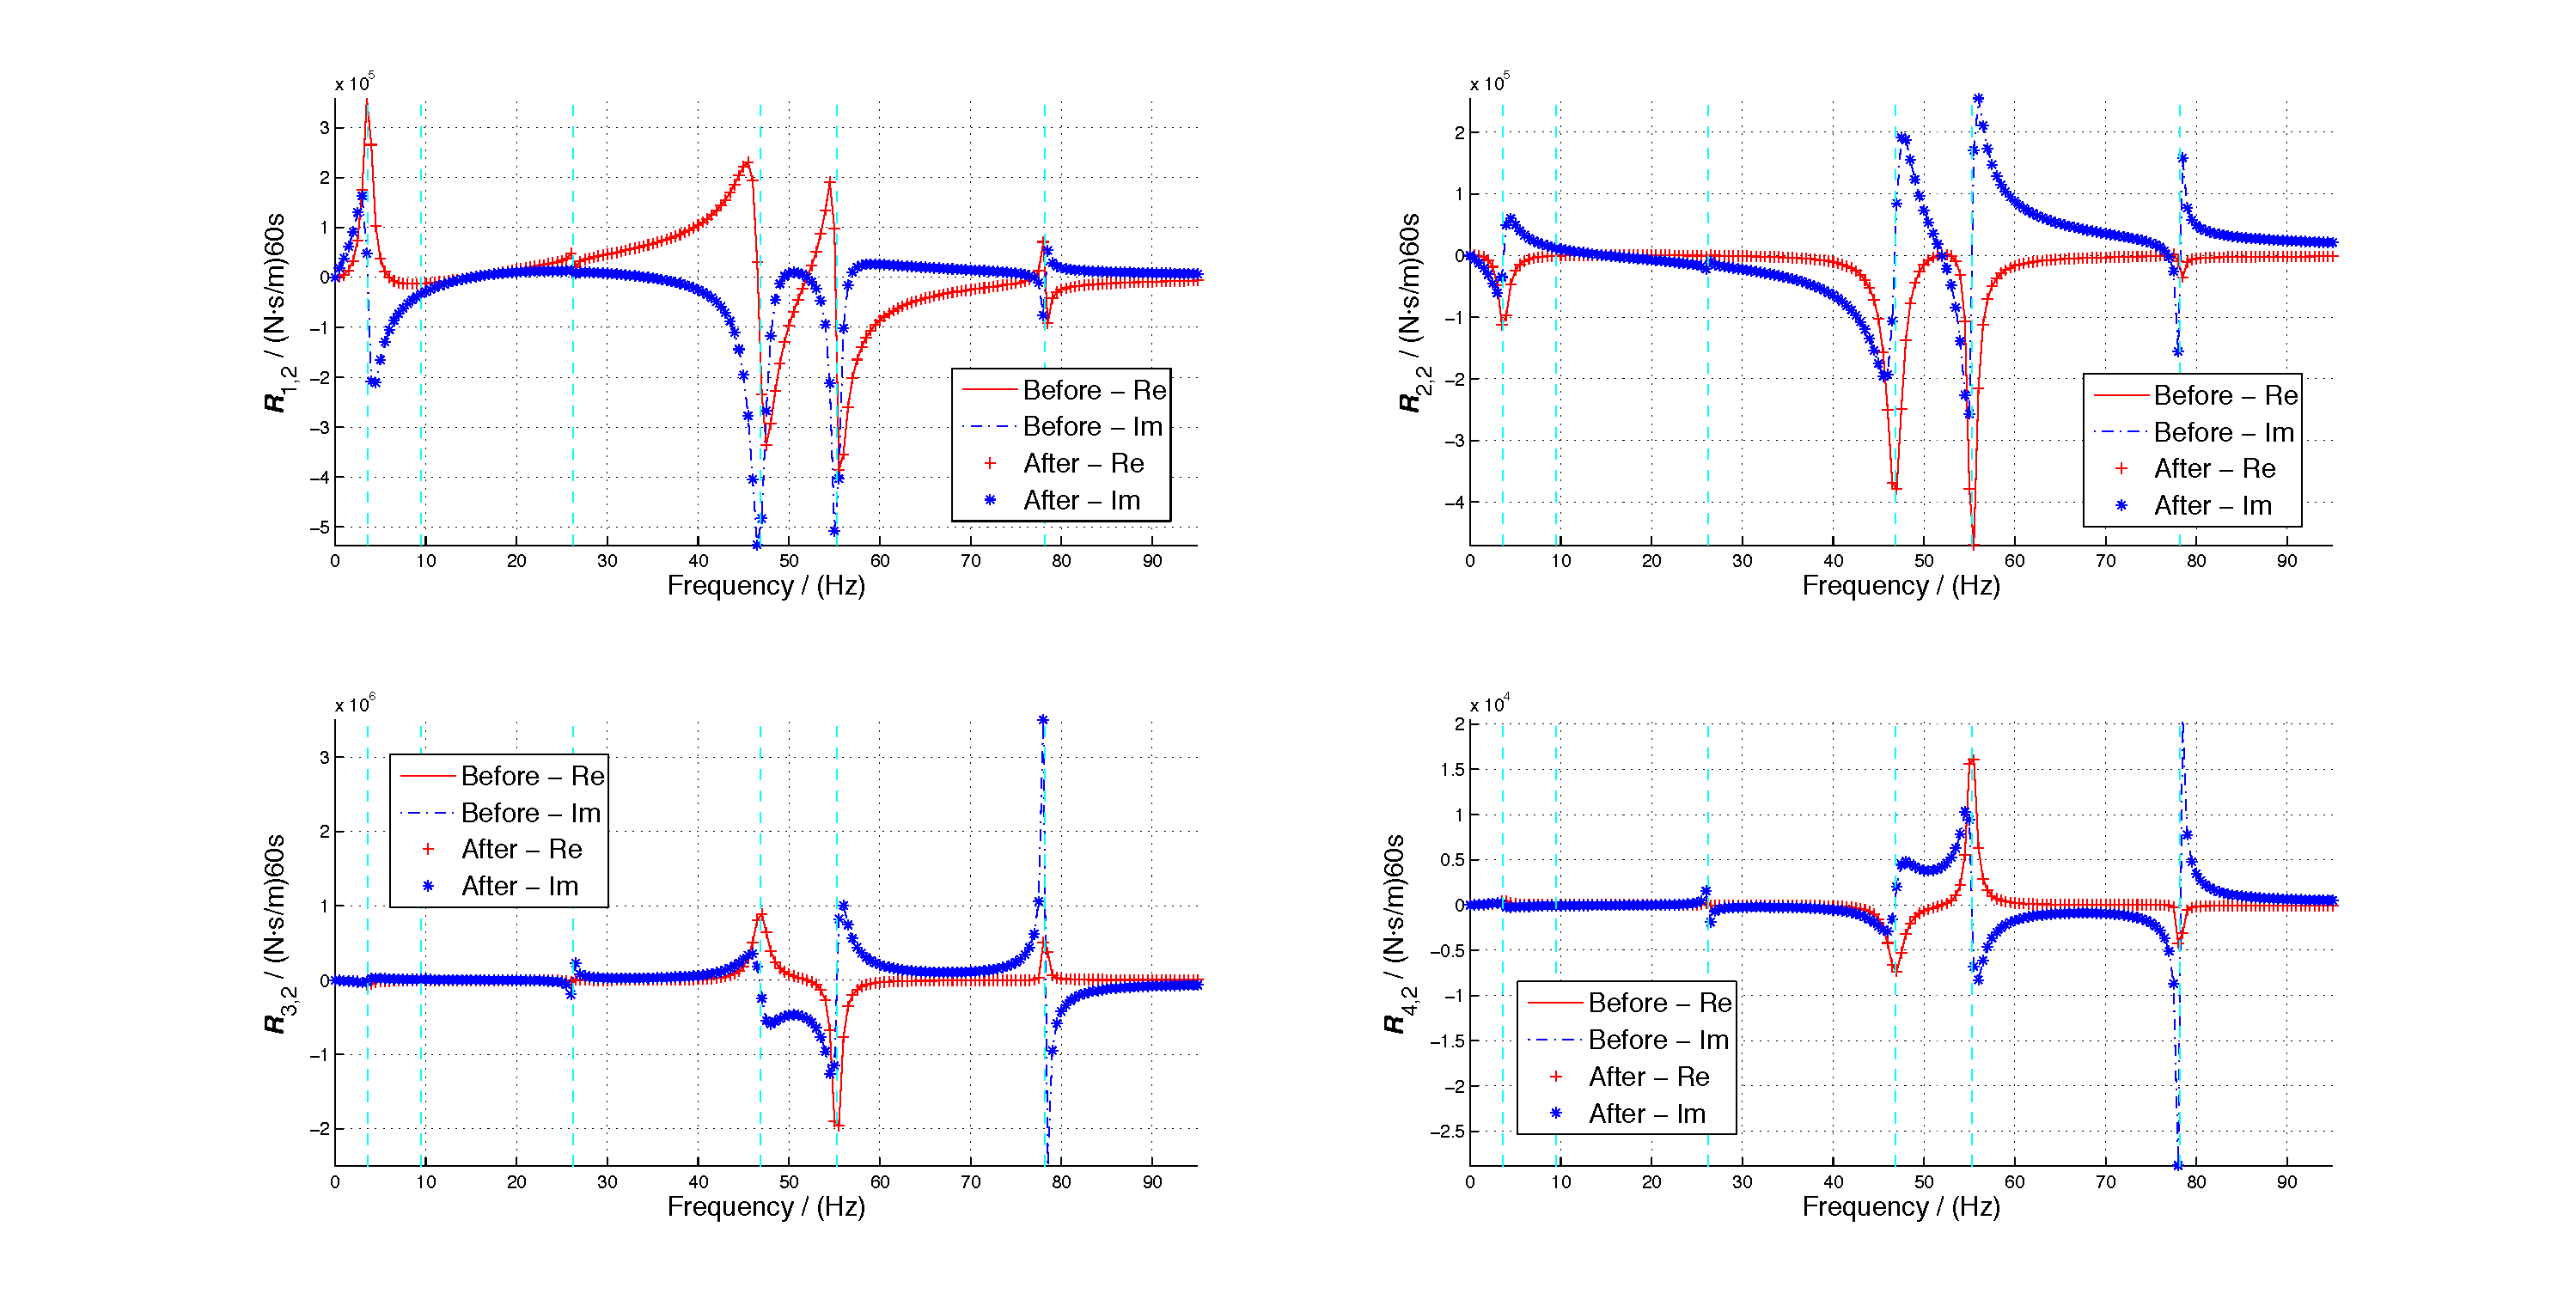
\includegraphics[trim={4.5cm 0cm 4.5cm 0cm}, clip=true, width=\linewidth]{Fitted-Transfer-02.pdf}
  \caption{管路系统反馈力有理分式拟合前后对比曲线(b):$\boldsymbol{R}_{12}-\boldsymbol{R}_{42}$}
  \label{Rational-Fitted-VS-02}
\end{figure}

至此,可以将推进系统作用到结构上的反馈力将表示为:
\begin{equation}
  \label{eq:Rational-Feedback-Force}
  \boldsymbol{F}_p(s)= \boldsymbol{R}_{pq}(s)\boldsymbol{\dot{X}}_q(s)
  =\left[ s\boldsymbol{M}_{pq}+ \boldsymbol{D}_{pq}+ \sum_{k=1}^n
    \left( \frac{\boldsymbol{C}_{pq}^{(k)}}{s-{A}_k} +
    \frac{\bar{\boldsymbol{C}}_{pq}^{(k)}}{s-\bar{A}_k}  \right)
    \right] \boldsymbol{\dot{X}}_q(s)
\end{equation}
其中$\boldsymbol{M}_{pq}, \boldsymbol{D}_{pq}$为实矩阵,${A}_k$为成对的共轭极点,$\boldsymbol{C}_{pq}^{(k)}$为成对的共轭矩阵,$p,q$分别表示阻抗矩阵的行数和列数,既管路系统反馈力和结构系统速度反馈节点的个数。在通常情况下,由于振动分析很少关注传递函数中包含纯实极点的情况,所以在拟合反馈力传递函数的时候并没有添加$R_j$项。

\subsection{反馈力传递矩阵的类结构化建模}
经过上节有理分式的拟合过程,管路系统反馈力传递函数已经被表示为了形如公式\eqref{eq:Rational-Feedback-Force}的较为简单形式。接下来,考虑对其进行进一步等效变换,通过引入辅助变量将有理分式转化为与结构振动方程相似的二阶常微分方程形式,便于进行下一步的耦合系统快速特征值求解。为此,考察$\boldsymbol{R}_{pq}(s)$其中一对共轭项:
\begin{equation}
  \label{eq:Feedback-Force-Original}
  \boldsymbol{F}_p^{(k)}(s)=\left( \frac{\boldsymbol{C}_{pq}^{(k)}}{s-A_k}+ \frac{\bar{\boldsymbol{C}}_{pq}^{(k)}}{s-\bar{A}_k} \right) \dot{\boldsymbol{X}_q}(s)
\end{equation}
对矩阵$\boldsymbol{C}_{pq}^{(k)}$做奇异值分解\cite{Golub:1996}
\begin{equation}
  \label{eq:QR-Dissect}
  \boldsymbol{C}_{pq}^{(k)}=\boldsymbol{U}_{pp}^{(k)}\boldsymbol{S}_{pq}^{(k)}{\boldsymbol{V}_{qq}^{(k)}}^{*}
\end{equation}
此处${}^*$表示矩阵的共轭转置,$\boldsymbol{S}_{pq}^{(k)}$形式如下
\begin{equation}
  \label{eq:SVD-Rank-Analysis}
  \boldsymbol{S}_{pq}^{(k)}=\left[ \begin{matrix}
      \boldsymbol{S}_{r_kr_k}^{(k)} & \boldsymbol{0}_{r_k(q-r_k)}     \\
      \boldsymbol{0}_{(p-r_k)}      & \boldsymbol{0}_{(p-r_k)(q-r_k)} \\
    \end{matrix} \right]
\end{equation}
$r_k$为矩阵$\boldsymbol{C}_{pq}^{(k)}$的秩,$\boldsymbol{S}_{r_kr_k}^{(k)}$为非奇异实对角矩阵,$\boldsymbol{U}_{pp}^{(k)}, \boldsymbol{V}_{qq}^{(k)}$为复矩阵,满足:
\begin{equation}
  {\boldsymbol{U}_{pp}^{(k)}}^*\boldsymbol{U}_{pp}^{(k)}=\boldsymbol{I}_{pp},
  {\boldsymbol{V}_{qq}^{(k)}}^*\boldsymbol{V}_{qq}^{(k)}=\boldsymbol{I}_{qq}
\end{equation}
分别从矩阵$\boldsymbol{U}_{pp}^{(k)}, \boldsymbol{V}_{qq}^{(k)}$中取出前$r_k$列,构成列满秩矩阵$\boldsymbol{U}_{pr_k}^{(k)}, \boldsymbol{V}_{qr_k}^{(k)}$,将公式\eqref{eq:QR-Dissect}表示成
\begin{equation}
  \boldsymbol{C}_{pq}^{(k)}=\boldsymbol{U}_{pr_k}^{(k)}\boldsymbol{S}_{r_kr_k}^{(k)}{\boldsymbol{V}_{qr_k}^{(k)}}^{*}
\end{equation}
这样,可以将推进系统反馈力$\boldsymbol{F}_p^{(k)}(s)$改写为:
\begin{equation}
  \label{eq:Single-SVD-Feedback-Force}
  \boldsymbol{F}_p^{(k)}(s)=\left( \frac{
  \boldsymbol{U}_{pr_k}^{(k)}\boldsymbol{S}_{r_kr_k}^{(k)}{\boldsymbol{V}_{qr_k}^{(k)}}^{*}
  }{s-A_k}+ \frac{
  \boldsymbol{\bar{U}}_{pr_k}^{(k)}\boldsymbol{S}_{r_kr_k}^{(k)}{\boldsymbol{\bar{V}}}{{}_{qr_k}^{(k)}}^{*}
  }{s-\bar{A}_k} \right) \dot{\boldsymbol{X}_q}(s)
\end{equation}

\noindent 定义两组关于时间的实函数$\boldsymbol{y}_{r_k}^{\prime(k)}(t), \boldsymbol{y}_{r_k}^{\prime\prime(k)}(t)$,在时域满足微分方程
\begin{equation}
  \label{eq:Extra-Variable-ODE}
  \left\{
  \begin{aligned}
    \dot{\boldsymbol{y}}_{r_k}^{\prime(k)}(t)- A'_k\boldsymbol{y}_{r_k}^{\prime(k)}(t)+A''_k\boldsymbol{y}_{r_k}^{\prime\prime(k)}(t)       & = {\boldsymbol{V}_{qr_k}^{\prime(k)}}^{\ut} \boldsymbol{x}_{q}(t)        \\
    \dot{\boldsymbol{y}}_{r_k}^{\prime\prime(k)}(t)-A''_k \boldsymbol{y}_{r_k}^{\prime(k)}(t)-A'_k\boldsymbol{y}_{r_k}^{\prime\prime(k)}(t) & = -{\boldsymbol{V}_{qr_k}^{\prime\prime(k)}}^{\ut} \boldsymbol{x}_{q}(t)
  \end{aligned} \right.
\end{equation}
其中,复数变量的记号约定同上节:$A'_k=\Re(A_k),A''_k=\Im(A_k)$,复矩阵在写法上亦采用相同规范
\begin{displaymath}
  \boldsymbol{V}_{qr_k}^{\prime(k)}=\Re(\boldsymbol{V}_{qr_k}^{(k)}), \boldsymbol{V}_{qr_k}^{\prime\prime(k)}=\Im(\boldsymbol{V}_{qr_k}^{(k)})
\end{displaymath}
$\boldsymbol{x}_q(t)$是$\boldsymbol{X}_q(s)$的Laplace逆变换:
\begin{displaymath}
  \boldsymbol{x}_q(t)=\Lacelap{\boldsymbol{X}_q(s)}
\end{displaymath}
将公式\eqref{eq:Extra-Variable-ODE}进行Laplace变换,
\begin{equation}
  \label{eq:Extra-Variable-Laplace}
  \left\{
  \begin{aligned}
    (s-A'_k)\boldsymbol{Y}_{r_k}^{\prime(k)}(s)+ A''_k\boldsymbol{Y}_{r_k}^{\prime\prime(k)}(s)  & ={\boldsymbol{V}_{qr_k}^{\prime(k)}}^{\ut}\boldsymbol{X}_q(s)         \\
    -A''_k\boldsymbol{Y}_{r_k}^{\prime(k)}(s)+ (s-A'_k)\boldsymbol{Y}_{r_k}^{\prime\prime(k)}(s) & = -{\boldsymbol{V}_{qr_k}^{\prime\prime(k)}}^{\ut}\boldsymbol{X}_q(s)
  \end{aligned} \right.
\end{equation}
其中
\begin{align}
  \boldsymbol{Y}_{r_k}^{\prime(k)}(s)       & =\Laplace{\boldsymbol{y}_{r_k}^{\prime(k)}(t)} \nonumber       \\
  \boldsymbol{Y}_{r_k}^{\prime\prime(k)}(s) & =\Laplace{\boldsymbol{y}_{r_k}^{\prime\prime(k)}(t)} \nonumber \\
  \boldsymbol{X}_q(s)                       & = \Laplace{\boldsymbol{x}_q(t)} \nonumber
\end{align}
可以验证,满足方程\eqref{eq:Extra-Variable-Laplace}的函数$\boldsymbol{Y}_{r_k}^{\prime(k)}, \boldsymbol{Y}_{r_k}^{\prime\prime(k)}$必然满足:
\begin{subequations}
  \label{eq:Extra-Variable-Laplace-Displacement}
  \begin{align}
    {\displaystyle\frac{{\boldsymbol{V}_{qr_k}^{(k)}}^{*}}{(s-A_k)}} \boldsymbol{X}_q(s)               & = \boldsymbol{Y}_{r_k}^{\prime(k)}(s)+ \jmath\boldsymbol{Y}_{r_k}^{\prime\prime(k)}(s)  \label{eq:Extra-Variable-Laplace-Displacement-01} \\
    {\displaystyle\frac{\boldsymbol{\bar{V}}{{}_{qr_k}^{(k)}}^{*}}{(s-\bar{A}_k)}} \boldsymbol{X}_q(s) & = \boldsymbol{Y}_{r_k}^{\prime(k)}(s)- \jmath\boldsymbol{Y}_{r_k}^{\prime\prime(k)}(s)  \label{eq:Extra-Variable-Laplace-Displacement-02}
  \end{align}
\end{subequations}
将公式\eqref{eq:Extra-Variable-Laplace-Displacement}带入\eqref{eq:Single-SVD-Feedback-Force},$\boldsymbol{F}_p^{(k)}(s)$可以写为:
\begin{equation}
  \label{eq:Feedback-Single-Force-Extra-Variable}
  \boldsymbol{F}_p^{(k)}(s)=2\left[ \boldsymbol{U}_{pr_k}^{\prime(k)}\boldsymbol{S}_{r_kr_k}^{(k)} \dot{\boldsymbol{Y}}_{r_k}^{\prime(k)}(s)-
    \boldsymbol{U}_{pr_k}^{\prime\prime(k)}\boldsymbol{S}_{r_kr_k}^{(k)} \dot{\boldsymbol{Y}}_{r_k}^{\prime\prime(k)}(s)
    \right]
\end{equation}
观察方程\eqref{eq:Extra-Variable-Laplace-Displacement-01},可以看出
\begin{equation}
  \label{eq:Extra-Variable-Displacement-Final}
  \boldsymbol{Y}_{r_k}^{\prime\prime(k)}(s)= {\displaystyle\frac{{\boldsymbol{V}_{qr_k}^{\prime(k)}}^{\ut} \boldsymbol{X}_q(s)-(s-A'_k)\boldsymbol{Y}_{r_k}^{\prime(k)}(s)}{A''_k}}
\end{equation}
若将\eqref{eq:Extra-Variable-Displacement-Final}分别带入公式\eqref{eq:Feedback-Single-Force-Extra-Variable}和\eqref{eq:Extra-Variable-Laplace-Displacement-02},可以导出
\begin{equation}
  \label{eq:Feedback-Force-Final}
  \left\{
  \begin{aligned}
    s\boldsymbol{D}_{pq}^{(k)}\boldsymbol{X}_{q}(s)+ s^2\boldsymbol{M}_{pr_k}^{(k)}\boldsymbol{Y}_{r_k}^{\prime(k)}(s)+ s\boldsymbol{D}_{pr_k}^{(k)}\boldsymbol{Y}_{r_k}^{\prime(k)}(s) & = \boldsymbol{F}_{p}^{(k)}(s) \\
    s^{2}\boldsymbol{Y}_{r_k}^{\prime(k)}(s)-s{\boldsymbol{V}_{qr_k}^{\prime(k)}}^{\ut} \boldsymbol{X}_{q}(s)- 2sA'_k\boldsymbol{Y}_{r_k}^{\prime(k)}(s)                                                                \\
    \qquad {} + \boldsymbol{K}_{r_kq}^{(k)}\boldsymbol{X}_{q}(s)+ ({A'_k}^2+{A''_k}^{2})\boldsymbol{Y}_{r_k}^{\prime(k)}(s)                                                             & =  \boldsymbol{0}_{r_k}
  \end{aligned} \right.
\end{equation}
其中,
\begin{displaymath}
  \begin{aligned}
    \boldsymbol{M}_{pr_k}^{(k)}=\frac{2}{A''_k} \boldsymbol{U}_{pr_k}^{\prime\prime(k)} \boldsymbol{S}_{r_kr_k}^{(k)}                                          & , \; \boldsymbol{K}_{r_kq}^{(k)}= {A'_k} {\boldsymbol{V}_{qr_k}^{\prime(k)}}^{\ut}- {A''_k}{\boldsymbol{V}_{qr_k}^{\prime\prime(k)}}^{\ut}                             \\
    \boldsymbol{D}_{pq}^{(k)}=-\frac{2}{A''_k} \boldsymbol{U}_{pr_k}^{\prime\prime(k)} \boldsymbol{S}_{r_kr_k}^{(k)} {\boldsymbol{V}_{qr_k}^{\prime(k)}}^{\ut} & , \; \boldsymbol{D}_{pr_k}^{(k)}=\frac{2}{A''_k}(A''_{k}\boldsymbol{U}_{pr_k}^{\prime(k)}- {A'_k}\boldsymbol{U}_{pr_k}^{\prime\prime(k)})\boldsymbol{S}_{r_kr_k}^{(k)}
  \end{aligned}
\end{displaymath}
考察公式\eqref{eq:Feedback-Force-Final},若将方程组中的变量$\boldsymbol{Y}_{r_k}^{\prime(k)}(s)$消去,将得到与公式\eqref{eq:Feedback-Force-Original}形式相同的推进系统反馈力$\boldsymbol{F}_p^{(k)}(s)$与结构反馈速度$\dot{\boldsymbol{X}}_q(s)$传递关系,因此方程\eqref{eq:Feedback-Force-Final}与\eqref{eq:Feedback-Force-Original}在数学上是等价的。

在实际操作过程当中,通常可以观察到公式\eqref{eq:SVD-Rank-Analysis}中$\boldsymbol{S}_{r_kr_k}^{(k)}$的元素存在如下规律:$\alpha_1\gg\alpha_n,\ n=2\dots r_k$\footnote{在SVD分解的过程中,按照常见的做法将奇异值由大而小排列}。
\begin{displaymath}
  \boldsymbol{S}_{r_kr_k}^{(k)}= \begin{bmatrix}
    \rule{2pt}{0ex}\alpha_1                                           &        & \text{\raisebox{-1.2ex}{\makebox[0pt][c]{\huge0}}} \\[0em]
                                                                      & \ddots &                                                    \\[0em]
    \text{\rule{1pt}{0ex}\raisebox{-0.4ex}{\makebox[0pt][c]{\huge0}}} &        & \alpha_{r_k}                                       \\[0em]
  \end{bmatrix}
\end{displaymath}
为了尽量减少辅助变量$\boldsymbol{Y}_{r_k}^{\prime(k)}$的个数\footnote{辅助变量的总数为:$\sum_{k=1}^n r_n$,既$\boldsymbol{S}_{r_kr_k}^{(k)}$非零奇异值数目之和},在不显著影响传递关系精度的情况下可以将除$\alpha_1$之外的奇异值置零。

利用方程\eqref{eq:Feedback-Force-Final},一般形式的管路系统反馈力传递函数\eqref{eq:Rational-Feedback-Force}最终可以等效成为:
\begin{equation}
  \label{eq:Final-Common-Feedback-SVD-Force}
  \left\{
  \begin{aligned}
     & ({s}^{2}{\boldsymbol{M}_{pq}}+s{\boldsymbol{C}_{pq}})\boldsymbol{X}_{q}(s)+({s}^{2}\boldsymbol{M}_{pr_T}+s{\boldsymbol{B}_{pr_T}})\boldsymbol{Y}_{r_T}(s)=\boldsymbol{F}_{p}(s)                            \\
     & (s\boldsymbol{V}_{r_Tq}+\boldsymbol{K}_{r_Tq})\boldsymbol{X}_{q}(s)+(s^2\boldsymbol{I}_{r_Tr_T}+s\boldsymbol{\Lambda}_{r_Tr_T} + \boldsymbol{\Omega}_{r_Tr_T})\boldsymbol{Y}_{r_T}(s)=\boldsymbol{0}_{r_T}
  \end{aligned} \right.
\end{equation}
其中
\begin{displaymath}
  \begin{aligned}
     & \boldsymbol{C}_{pq}=\boldsymbol{D}_{pq}+\sum_{k=1}^{n}{\boldsymbol{D}_{pq}^{(k)}} ,\
    \boldsymbol{M}_{pr_T}=\left[ \begin{matrix}
        \boldsymbol{M}_{pr_1}^{(1)} & \cdots & \boldsymbol{M}_{pr_n}^{(n)}
      \end{matrix} \right] ,\
    \boldsymbol{B}_{pr_T}=\left[ \begin{matrix}
        \boldsymbol{D}_{pr_1}^{(1)} & \cdots & \boldsymbol{D}_{pr_n}^{(n)}
      \end{matrix} \right]                         \\
     & \boldsymbol{K}_{r_Tq}=\left[ \begin{matrix}
        {\boldsymbol{K}_{r_1q}^{(1)}}^{\ut} \\
        \vdots                              \\
        {\boldsymbol{K}_{r_nq}^{(n)}}^{\ut}
      \end{matrix} \right], \
    \boldsymbol{V}_{r_Tq}=\left[ \begin{matrix}
        -{\boldsymbol{V}_{qr_1}^{\prime(1)}}^{\ut} \\
        \vdots                                     \\
        -{\boldsymbol{V}_{qr_n}^{\prime(n)}}^{\ut}
      \end{matrix} \right], \
    \boldsymbol{Y}_{r_T}(s)=\left[ \begin{matrix}
        \boldsymbol{Y}_{r_1}^{\prime(1)}(s) \\
        \vdots                              \\
        \boldsymbol{Y}_{r_n}^{\prime(n)}(s)
      \end{matrix} \right],\
    r_T= \sum_{k=1}^n r_n                                                                   \\
     & \boldsymbol{\Omega}_{r_Tr_T}=\operatorname{diag} \left(
    \begin{matrix}
        ({A}_{1}^{\prime 2}+{A}^{\prime\prime 2}_{1}) \boldsymbol{I}_{r_1} & \cdots & ({A}_{n}^{\prime 2}+{A}_{n}^{\prime\prime 2})\boldsymbol{I}_{r_n}
      \end{matrix}
    \right)                                                                                 \\
     & \boldsymbol{\Lambda}_{r_Tr_T}=\operatorname{diag}\left(
    \begin{matrix}
        -2A'_{1}\boldsymbol{I}_{r_1} & \cdots & -2{A'_{n}}\boldsymbol{I}_{r_n}
      \end{matrix}
    \right)
  \end{aligned}
\end{displaymath}

为了验证公式\eqref{eq:Final-Common-Feedback-SVD-Force}与原始管路系统反馈力传递函数\eqref{eq:Feedback-Force-Transfer}之间的等价性,图\ref{SVD-Fitted-VS-01}和\ref{SVD-Fitted-VS-02}仿照之前做法(同样为液体火箭升空后60s),给出了两种结果之间的对比曲线。可以看出,即使此处强制使得$\alpha_n=0,\ n=2\dots r_k$,既$\boldsymbol{C}_{pq}^{(k)}$秩为一,拟合后的反馈力阻抗曲线依然可以达到很高的精度\footnote{若对比曲线之间相差较大,可以采用最小二乘法对于$\alpha_1$关于原始采样数据进行修正}。

至此,若将经过类结构化处理的管路系统反馈力表达式\eqref{eq:Final-Common-Feedback-SVD-Force}代入结构系统有限元模型的运动方程\eqref{eq:Coupled-System-Transfer},最终可以得到Laplace域的耦合系统动力学方程:
\begin{equation}
  \label{eq:Final-Coupled-System-Laplace}
  \left\{
  \begin{aligned}
    (s^2\boldsymbol{M}_{ss}+ s\boldsymbol{C}_{ss}+ \boldsymbol{K}_{s}) \boldsymbol{X}_{s}(s)+(s^2\boldsymbol{M}_{sr_T}+s\boldsymbol{B}_{sr_T}) \boldsymbol{Y}_{r_T}(s)                    & =\boldsymbol{F}_{s}(s) \\
    (s\boldsymbol{V}_{r_Ts}+\boldsymbol{K}_{r_Ts})\boldsymbol{X}_{s}(s)+(s^2\boldsymbol{I}_{r_Tr_T}+s\boldsymbol{\Lambda}_{r_Tr_T}+\boldsymbol{\Omega}_{r_Tr_T})\boldsymbol{Y}_{r_{T}}(s) & =\boldsymbol{0}_{r_T}
  \end{aligned} \right.
\end{equation}
其中
\begin{displaymath}
  \begin{aligned}
     & \boldsymbol{M}_{ss}=\boldsymbol{M}_{s}-\boldsymbol{L}_{sp}\boldsymbol{M}_{pq}\boldsymbol{L}_{qs},\
    \boldsymbol{M}_{sr_T}=-\boldsymbol{L}_{sp}\boldsymbol{M}_{pr_T},\
    \boldsymbol{K}_{r_Ts}=\boldsymbol{K}_{r_Tq}\boldsymbol{L}_{qs}                                        \\
     & \boldsymbol{B}_{sr_{T}}=-\boldsymbol{L}_{sp}\boldsymbol{B}_{pr_T},\
    \boldsymbol{C}_{ss}=\boldsymbol{C}_{s}+\dot{\boldsymbol{M}}_s -\boldsymbol{L}_{sp}\boldsymbol{C}_{pq}\boldsymbol{L}_{qs},\
    \boldsymbol{V}_{r_Ts}=\boldsymbol{V}_{r_Tq}\boldsymbol{L}_{qs}
  \end{aligned}
\end{displaymath}
若将上式变换到时域,可以得到类似于常规结构系统的耦合系统动力学方程
\begin{equation}
  \label{eq:Final-Coupled-1D-Transfer}
  \boldsymbol{M}_c\ddot{\boldsymbol{x}}_c+\boldsymbol{C}_c\dot{\boldsymbol{x}}_c+\boldsymbol{K}_c\boldsymbol{x}_c=\boldsymbol{f}_c(t)
\end{equation}
其中
\begin{displaymath}
  \begin{aligned}
     & \boldsymbol{x}_{c}=\left[ \begin{matrix}
        \boldsymbol{x}_{s}   \\
        \boldsymbol{y}_{r_T} \\
      \end{matrix} \right],\
    \boldsymbol{f}_c(t)=\left[ \begin{matrix}
        \boldsymbol{f}_{s}(t) \\
        \boldsymbol{0}_{r_T}  \\
      \end{matrix} \right],\
    \boldsymbol{M}_{c}=\left[ \begin{matrix}
        \boldsymbol{M}_{ss}   & \boldsymbol{M}_{sr_T}   \\
        \boldsymbol{0}_{r_Ts} & \boldsymbol{I}_{r_Tr_T} \\
      \end{matrix} \right]      \\
     & \boldsymbol{C}_{c}=\left[ \begin{matrix}
        \boldsymbol{C}_{ss}   & \boldsymbol{B}_{sr_T}         \\
        \boldsymbol{V}_{r_Ts} & \boldsymbol{\Lambda}_{r_Tr_T}
      \end{matrix} \right],\
    \boldsymbol{K}_{c}=\left[ \begin{matrix}
        \boldsymbol{K}_{s}    & \boldsymbol{0}_{sr_T}        \\
        \boldsymbol{K}_{r_Ts} & \boldsymbol{\Omega}_{r_Tr_T} \\
      \end{matrix} \right]
  \end{aligned}
\end{displaymath}
方程\eqref{eq:Final-Coupled-1D-Transfer}的特征值可采用状态空间方法进行求解。令$\boldsymbol{y}_c=\dot{\boldsymbol{x}}_c,\ \boldsymbol{z}={[ {\boldsymbol{y}_c}^{\ut}\quad {\boldsymbol{x}_c}^{\ut} ]}^{\ut}$,可以将其改写为:
\begin{equation}
  \boldsymbol{A}\dot{\boldsymbol{z}}+ \boldsymbol{B}\boldsymbol{z}=\boldsymbol{f}(t)
\end{equation}
其中
\begin{displaymath}
  \boldsymbol{A}=\left[ \begin{matrix}
      \boldsymbol{0}     & \boldsymbol{M}_{c} \\
      \boldsymbol{M}_{c} & \boldsymbol{C}_{c} \\
    \end{matrix} \right],\
  \boldsymbol{B}=\left[ \begin{matrix}
      -\boldsymbol{M}_{c} & \boldsymbol{0}     \\
      \boldsymbol{0}      & \boldsymbol{K}_{c} \\
    \end{matrix} \right],\
  \boldsymbol{f}(t)=\left[ \begin{matrix}
      \boldsymbol{0}        \\
      \boldsymbol{f}_{c}(t) \\
    \end{matrix} \right]
\end{displaymath}
最后,耦合系统的特征值求解便可归结为矩阵特征值问题:
\begin{equation}
  \label{eq:Fast-Matrix-Eigen-Equation}
  \left( \lambda \boldsymbol{A}+ \boldsymbol{B} \right)\boldsymbol{\psi}_c=0
\end{equation}

\section{算例分析}
\label{sec:Lumped-Numerical-Simulation}
综合前述的矩阵闭环POGO稳定性分析方法和基于有理分式拟合及管路系统类结构化建模的快速特征值求解方法,液体火箭管路与结构耦合系统的特征值可以通过求解以下两种方程得到:非线性代数特征值问题\eqref{eq:Coupled-Transfer-Det}或矩阵特征值问题\eqref{eq:Fast-Matrix-Eigen-Equation}。为了验证该快速特征值求解方法是否准确,下面给出了两种方法根据虚部绝对值排序的耦合系统特征值对比表格(\ref{table:Direct-Fast-Comparison})。采用时间冻结手段(液体火箭升空后60s),计算工况考查了某液体火箭两输入(箱底和泵的反馈速度)、四输出(参考第\pageref{Page:Typical-Feedback-Force}页管路系统反馈力分类)单推进剂管路系统与结构系统的耦合振动特性。

\begin{table}[htp]
  \renewcommand{\arraystretch}{1.5}
  \centering
  \caption{矩阵闭环判别法与快速特征值求解法结果对比}
  \label{table:Direct-Fast-Comparison}
  \begin{tabularx}{\textwidth}{c>{\centering}X>{\centering}Xc}
    \toprule
    序号        & 矩阵闭环法(\si{\radian\per\s})        & 快速求解法(\si{\radian\per\s})       & 相对误差                                                                                                                       \\
    k           & $ s_k^{(\mathrm{\RNum{1}})}\cdot10^{3}$ & $s_k^{(\mathrm{\RNum{2}})}\cdot10^{3}$ & $\left| \frac{s_k^{(\mathrm{\RNum{2}})}-s_k^{(\mathrm{\RNum{1}})}}{s_k^{(\mathrm{\RNum{1}})}} \right| \cdot 100 \si{\percent}$ \\ \midrule
    \textbf{1 } & \num{-0.0039 + 0.0228i}                 & \num{-0.0039 + 0.0227i}                & \num{0.2164}                                                                                                                   \\
    \textbf{2 } & \num{-0.0016 + 0.0570i}                 & \num{-0.0017 + 0.0569i}                & \num{0.1414}                                                                                                                   \\
    \textbf{3 } & \num{-0.2154 + 0.0607i}                 & \num{-0.2153 + 0.0605i}                & \num{0.1279}                                                                                                                   \\
    \textbf{4 } & \num{-0.0051 + 0.0702i}                 & \num{-0.0049 + 0.0701i}                & \num{0.2621}                                                                                                                   \\
    \textbf{5 } & \num{-0.0067 + 0.1265i}                 & \num{-0.0066 + 0.1265i}                & \num{0.0079}                                                                                                                   \\
    \textbf{6 } & \num{-0.0002 + 0.1654i}                 & \num{-0.0002 + 0.1654i}                & \num{0.0121}                                                                                                                   \\
    \textbf{7 } & \num{-0.0161 + 0.2182i}                 & \num{-0.0179 + 0.2165i}                & \num{1.1249}                                                                                                                   \\
    \textbf{8 } & \num{-0.0248 + 0.2475i}                 & \num{-0.0248 + 0.2475i}                & \num{0.0180}                                                                                                                   \\
    \textbf{9 } & \num{-0.0351 + 0.2940i}                 & \num{-0.0351 + 0.2940i}                & \num{0.0068}                                                                                                                   \\
    \textbf{10} & \num{-0.0132 + 0.2970i}                 & \num{-0.0132 + 0.2963i}                & \num{0.2155}                                                                                                                   \\ \bottomrule
  \end{tabularx}
\end{table}

\begin{table}[htp]
  \renewcommand{\arraystretch}{1.5}
  \centering
  \caption{管路系统的主要特征参数}
  \label{table:Main-Feedline-Parameter}
  \begin{tabular}{>{$}c<{$}c>{$}c<{$}c:>{$}c<{$}c}
    \toprule
    \multicolumn{4}{c}{时不变参数} & \multicolumn{2}{c}{时变参数}                                                                                                                       \\
    \midrule
    A_T                            & 贮箱截面积                   & \rho     & 液体密度                                     & c^{(n)}                & 液路当地声速                     \\
    N                              & 发动机台数                   & C_f      & 有效推力系数                                 & h_T                    & 贮箱的液面高度                   \\
    A^{(n)}                        & 管路元件截面积               & L^{(n)}  & 管路元件惯性                                 & \rule{5pt}{0pt}C^{(3)} & 蓄压器柔度                       \\
    R^{(n)}                        & 管路元件阻力                 & Q_s      & 泵的稳态体积流                               & \rule{5pt}{0pt}C^{(5)} & 泵的气蚀柔度                     \\
    m                              & 泵的动力学增益               & \epsilon & \rule{4pt}{0pt}燃烧室压力时滞\rule{4pt}{0pt} & C^*                    & 燃烧室的特征速度 \tabularnewline
    \bottomrule
  \end{tabular}
\end{table}

\begin{figure}[!htb]
  \centering
  %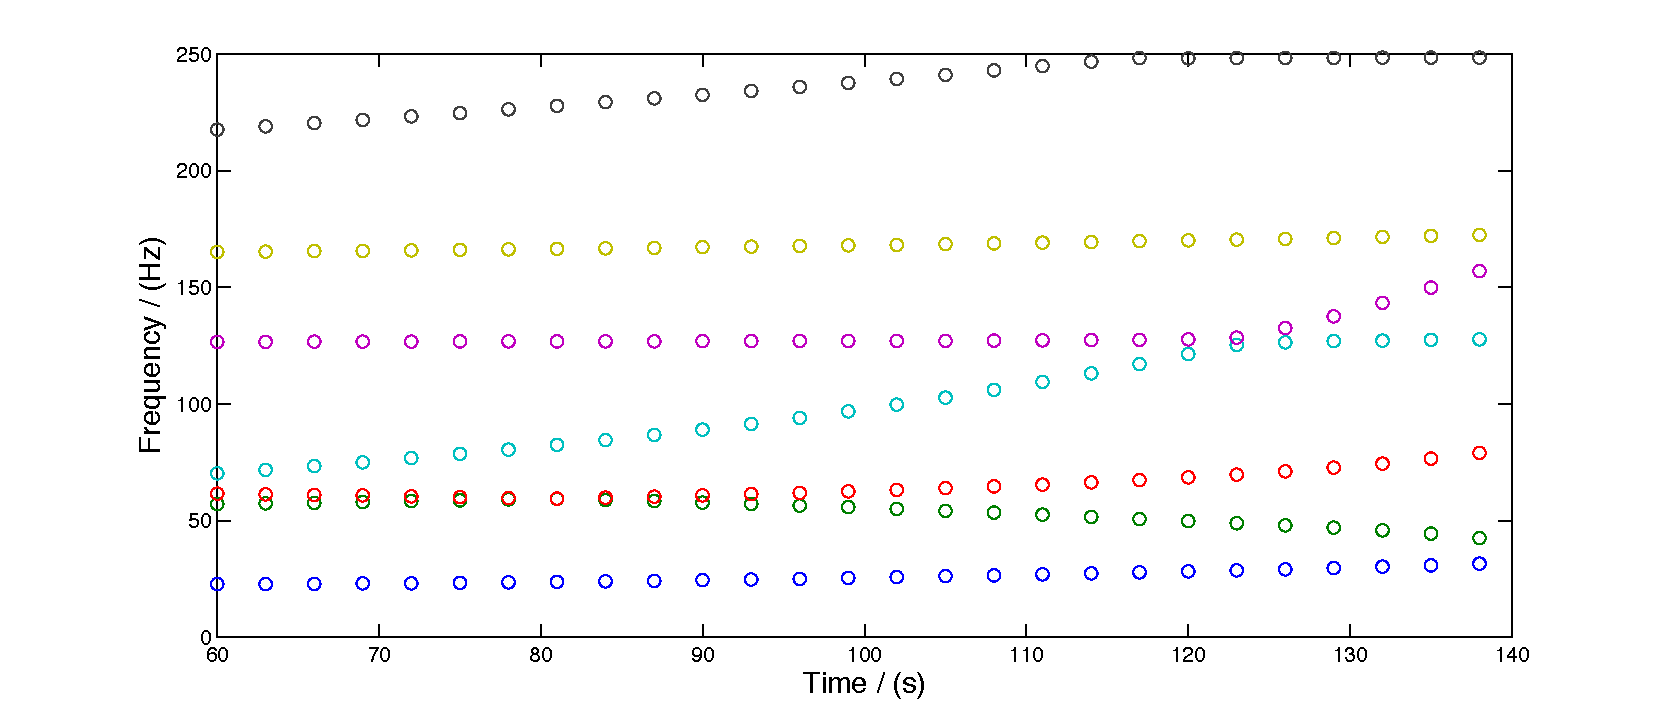
\includegraphics[trim={1.5cm 0cm 1.5cm 0cm}, clip=true, width=.92\linewidth]{Lumped-Frequency-Curve.pdf}
  \caption{耦合系统集中参数模型的固有频率变化曲线}\label{Lumped-Frequency-Curve}
\end{figure}

\begin{figure}[!htb]
  \centering
  %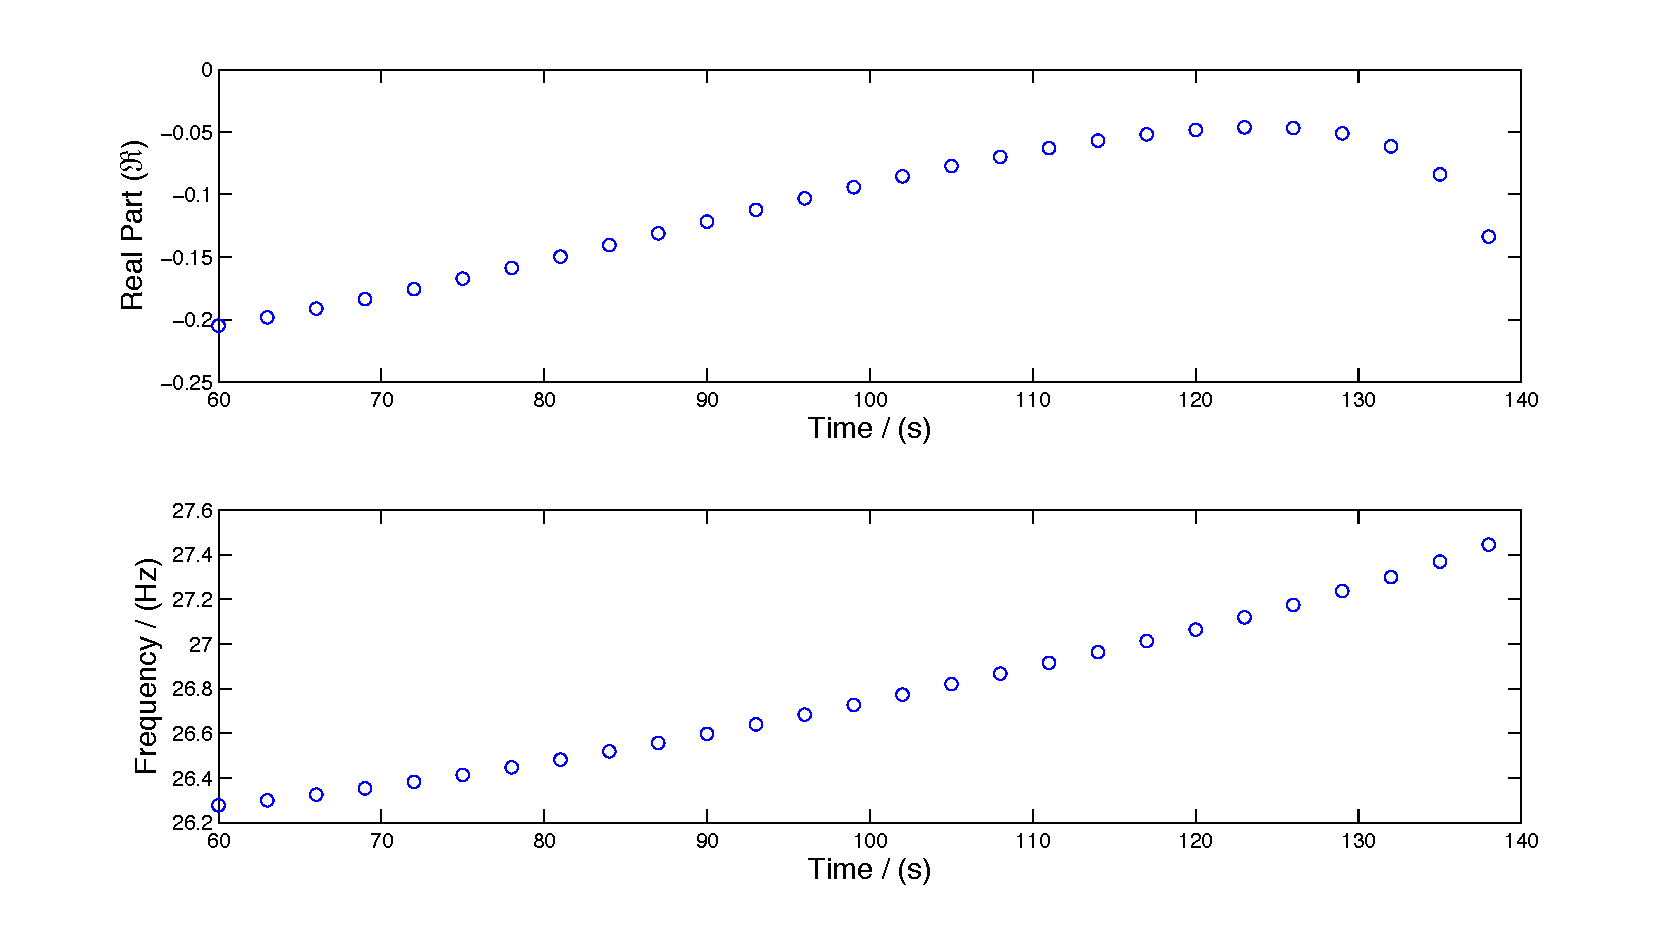
\includegraphics[trim={1.5cm 0.4cm 1.5cm 1cm}, clip=true, width=.92\linewidth]{Lumped-Max-Eigen-Curve.pdf}
  \caption{耦合系统集中参数模型的特征值变化曲线}\label{Lumped-Max-Eigen-Curve}
\end{figure}

\bibliographystyle{FDUbib}
\bibliography{ref}











% @Author: YangZhou
% @Date:   2017-06-30 15:05:00
% @Last Modified by:   YangZhou
% @Last Modified time: 2018-01-16 23:36:43

\chapter{集中参数模型的POGO稳定性分析}
由于接下来我们希望研究strain对热导率的影响,为了合理地选取strain,我们必须知道这个结构在什么时候处于弹性拉伸区,什么时候会断。因此我们首先做一个拉伸测试。
左上和左下图表明无论strain有多小,stress都不为0,由于knot的存在必须有一个初始拉伸,所以0.0的位置Stress不为0。体系的稳定性依赖于一个外界strain,在这个范围内stress和strain成指数关系。且这个拉伸关系与温度关系不明显。
右上的图表是的是从0的位置向右加strain到0.05,然后向左strain变到-0.15,再回到0.0。这个图类似于磁滞回线,表面knot的状态与加压的历史有关,但是0.05左右的时候体系只有一个状态,这也就是我们要研究的strain。
右下图的是graphene相应的结果,可见knot与graphene的拉伸性质很不一样。

这里我们来研究knot的断裂。
左上图是同一个knot在不同初始seed情况下的多次拉伸结果。可以发现0.07以下的时候,体系处于一个确定的状态,与初始情况无关。这个strain以后可以认为knot第一次断裂,但是断得并不彻底,而是发生了塑性形变,如
红色的那一根线,先后断裂了3次才彻底断裂。各次断裂之间表现出线性关系,有确定的杨氏模量,但Stress的起伏也变大,起伏的周期也与相应的阶段有关。
左下图表面了体系中的应力分布,主要集中在结的附近,因此总是结最先断裂。
右上图表示用来打结的graphene的长度对这个关系的影响。越长的体系断裂得也越是彻底,最初断裂的位置变化不大,但有一定的位移。这个图的结果表明我们对不同lx的knot取0.05以下的strain是合理的。
右下图是左上图的各个曲线(共600次)对应平均。在第一次断裂以后Stress出现一个小幅增长,接着迅速下降,且之后随着strain的增加下降得越来越慢。更多的结果表明这个下降满足反比关系,即使strain=1.0,Stress也并非彻底为0.这确实是一个塑性形变。而grapheen的断裂相当干脆,是一种脆性的断裂。


ps,我刚刚想到对不同lx,把右下角的图头画一遍,从而不会那么空
左上图绿色表示的是第一次断裂的时候体系处于某个strain的概率,这个概率相当集中,基本上就在0.07附近,展宽很小。而红色的表示第二次断裂的时候的strain分布,它的最高点大概在0.17,展宽更大,所以这阶段的体系的稳定性不确定,可能在第一次断裂后不久就断裂了,也可能要过挺久。第三和第四次断裂的密度基本重合,且分布十分广泛。
左下图表示的是strain从0到1.0 变化的范围内体系断裂的次数的统计情况。可以发现,体系在这个范围内很可能断裂2到3次,但最多的断裂了9次之多。
右下图表示体系在这个strain下彻底断裂的可能性。可已看出,体系第一次断裂就很彻底的概率很小,但并非没有。到0.3附件,断裂的概率有了一半,到1.0附件,体系基本上已经全部断裂。
右上图是对断裂之前和两次断裂之间的体系的杨氏模量的统计。225左右的可能性最大的情况就是体系断裂前的杨氏模量。对与断裂后的情况,杨氏模量普遍变小,集中在150以下,在此之后可能性逐渐降低。因此断裂以后体系反倒更加容易拉伸了。
从这里开始我们研究这个材料的传热性质。先是长度和strain对热导率的影响。
左图表示不同strain情况下构成knot的graphene的长度对这个单结系统热导率的影响。在当前的尺度上,热导随长度基本是线性变化的。strain对热导率的影响不大。
右图显式地得到不同lx热导与strain的关系,可见strain对热导率的影响不大。相比较而言,graphene的strain对热导率影响挺大(然后引你的文章)
然后看看界面热导与温差的关系。再研究这个热导随superlattice长度的关系。
左上:对于特定的lx=70,kapitza与温差间的关系,可见dT(两端温差的一半)达到20K以后界面热阻不再变化。
左下:上图的每个点对应的温度分布
右上:用lx=70的graphene构成的knot去构造superlattice,nx表示superlattice包含几个结。计算的时候dT=100,横截面积取的相同的值,后面我会改成你建议的热流。这个图表明tc随nx基本上线性增加,在计算能承受的范围内没有要收敛的迹象。综合这个图与之前tc~lx的结果,我们得出,即使出现了knot这样的缺陷,在计算可承受的范围内热导依然不会收敛。
右下:温度分布与nx间的关系,横坐标是归一化的x。随nx的增大,温度分布逐渐趋向线性关系,knot构成的微观细节逐渐被抹去,在大尺度上可以被看做质点,于是可以被抽象为一个一维点阵,因此用一维点阵的结论可得tc发散。
右下inset:每个knot导致的温差delT*nx与nx的关系。在nx比较小的时候,knot处的温度下降占总温差的一半左右,而nx增大后,几乎全部的温差降落都是在knot处出现的,非knot处几乎没有温度降落。
这一页是还没完成的工作,我是感觉前面的东西太过流水账,没有太深刻的分析(不过我感觉这是我现在能做到的最好的程度了)。所以希望从谱的方面做一些补充。
左上:用速度关联函数求出每个原子的dos,然后对knot的bulk区域和结的区域分别计算dos,得到蓝色和绿色的线。红色的为graphene的dos。这个结果表明结的影响是非局域的,它让整个区域上的dos都偏离了graphene的结果,而不仅仅是knot的区域。基于这个部分,我打算计算一个很长的knot的dos,然后按离结的远近画更多区域的dos,看画到多远那个dos会像graphene的,如过足够远都不行,我们可以得出结论:结的存在是完全非局域的。而如果会像graphene的,那就更好了,就可以求出这个关联长度lc,进一步再研究strain,T什么的对它的影响,就又可以凑几个图。
右上:结的dos按xyz的分解,
右下:graphene的dos按xyz的分解,目前看来这两个图的意义不大。

所以我想改进点的地方就是,应该加点什么图,哪些图又该不要,应该在哪些地方多下点功夫,使得这个工作显得更有意义一些?


\bibliographystyle{FDUbib}
\bibliography{ref}
% 
% \include{Chapter03}
% 
% % !TEX encoding = UTF-8 Unicode
%!TEX TS-program = xelatex

\chapter{结论与展望}

\section{全文总结}
乘着祖国大力发展载人航天事业的契机,本文以液体火箭纵向耦合振动的稳定性分析为主要研究内容,比较深入的阐述了POGO问题的研究对象、作用机理、求解方法及预防手段。全文研究工作的要点及创新点主要包括:
\begin{enumerate}[leftmargin=0pt, align=parleft, itemindent=2\parindent, labelsep=0pt, label=\roman*).]
	\item 较为全面的总结了国内、外液体火箭纵向耦合问题的研究进展,指出了传统的液体火箭POGO稳定性分析方法如矩阵法、单传法和临界阻尼法,在求解非对称、非线性复传递矩阵特征值时遇到的主要问题及方法局限性。
	\item 发展了一种基于矩阵法和有理分式拟合法的耦合系统快速特征值求解算法。该方法能够利用类结构化建模技术将包含超越函数的管路推进系统反馈力传递函数等效变换为与结构动力学方程一致的形式,通过求解矩阵特征值问题以快速、精确的确定耦合系统动力学稳定性。
	\item 利用虚质量法及带孔箱底精细有限元建模技术,提出了一套液体火箭带液贮箱的三维轴对称建模方法。发展后的三维带液贮箱模型不仅能够提供足够完整且合理的结构系统模态参与耦合计算,并且为管路系统提供了更为科学和精确的入口端边界条件。结合MSC.Nastran提供的传递函数TF卡建模工具,文章还给出了一种能够使得有理分式形式的反馈力传递函数参与结构系统耦合计算的商业软件整合技术,基本实现了耦合系统时变复特征值计算的模块化与自动化。
	\item 将液体火箭结构系统阻尼特性的识别和建模引入耦合系统稳定性分析,指出了适用于液体火箭POGO仿真的阻尼施加方式。通过调整贮箱干/湿面材料随时间变化的比例阻尼系数,成功的利用有限元模型模拟了实测贮箱阻尼结果。
	\item 通过比较不同类型的液体火箭在多种工况下的POGO稳定性分析结果,一方面揭示了耦合系统特征值与管路系统关键参数(如蓄压器容积等)之间的相互联系,另一方面还指出了将耦合系统动态传递特性分析纳入液体火箭POGO稳定性分析的重要性和必要性。参考现阶段国内液体火箭的设计水平与制造工艺,提出了一些分析及防治液体火箭POGO振动的基本思路,给出了液体火箭纵向耦合振动的理论分析框架和试验设计框架。
\end{enumerate}

\section{工作展望}
鉴于现有的理论基础和时间、经费及研究条件限制,本文的工作还存在许多不足及值得改进的地方:
\begin{enumerate}[leftmargin=0pt, align=parleft, itemindent=2\parindent, labelsep=0pt, label=\arabic*).]
	\item 管路推进系统只考虑了单组元的燃烧推力生成模型,尚没有考虑双贮箱情形的液体三维流动耦合作用;
	\item 一些管路系统元件的时变参数如泵的柔度与管件的当地声速,需要更为精确的实验测定;
	\item 耦合系统的结构阻尼时变参数需要进一步的理论分析及实验支持;
	\item 液体火箭结构系统仅对带液贮箱引入了三维有限元模型,其余部件依然采用集中参数弹簧-质量模型,需要进一步建立箭体结构其它部分的三维模型与贮箱进行匹配;
	\item 在对液体火箭管路系统进行建模时,未考虑蓄压器等元件的非线性效应;
	\item 未考虑液体火箭在结构失稳时由于非线性效应而产生的极限环现象;
	\item 程序、算法需要进一步完善和工程化。
\end{enumerate}

POGO振动本身是一个十分复杂的多领域、多系统、多参数的非线性时变问题。在与之配套的理论分析基础和实验测量数据都很不完备的今天,若期待祖国的载人航天事业能走的更远、更坚实,大量的后续工作还需要继往开来的科研工作者持之以恒的付出和实践。愿以此文与之共勉。


%----------------------------Appendix-------------------------------!
\appendix

\renewcommand{\thechapter}{附录{\Alph{chapter}}}

%\chapter{公式推导}

%----------------------------Back Matter-------------------------------!
\backmatter

\phantomsection
\addcontentsline{toc}{chapter}{\bibname}
%zhouyang\bibliographystyle{FDUbib}
%zhouyang\bibliography{ref}
%\nocite{*}

\backchapter{致谢}

\clearpage
\printindex

\end{document}